\documentclass{article}
\usepackage{microtype}
\usepackage{graphicx}
\usepackage{booktabs}
\usepackage{hyperref}
\usepackage{icml2026}
\usepackage{amsmath,amssymb,amsthm}
\usepackage[capitalize,noabbrev]{cleveref}
\usepackage{enumitem}
\usepackage{tcolorbox}
\hypersetup{colorlinks=true,linkcolor=[RGB]{24,64,140},citecolor=[RGB]{24,64,140},urlcolor=[RGB]{24,64,140},pdfauthor={},pdftitle={}}
\graphicspath{{figures/}}

\theoremstyle{plain}
\newtheorem{proposition}{Proposition}
\newtheorem{lemma}{Lemma}
\theoremstyle{remark}
\newtheorem{remark}{Remark}
\theoremstyle{definition}
\newtheorem{observation}{Observation}

% One switch for the self-citation of the authors' ICML 2026 workshop paper (research-writing section 19).
% Submission: \anonsubmissiontrue cites it as Anonymous with the title suppressed.
% Camera-ready: \anonsubmissionfalse cites it in full.
\newif\ifanonsubmission
\anonsubmissiontrue
\newcommand{\wscitet}{\ifanonsubmission\citet{anon2026workshop}\else\citet{noel2026workshop}\fi}
\newcommand{\wscitep}{\ifanonsubmission\citep{anon2026workshop}\else\citep{noel2026workshop}\fi}

% generated by analysis/icml_v2_numbers.py; do not edit
\providecommand{\pending}[1]{\textbf{[PENDING: #1]}}
\newcommand{\FusConfGemmaBfcl}{\ensuremath{+0.177}}
\newcommand{\FusConfGemmaGlaive}{\ensuremath{+0.160}}
\newcommand{\FusConfHiGemmaBfcl}{\ensuremath{+0.21}}
\newcommand{\FusConfHiGemmaGlaive}{\ensuremath{+0.22}}
\newcommand{\FusConfHiLlamaOneBBfcl}{\ensuremath{+0.21}}
\newcommand{\FusConfHiLlamaOneBGlaive}{\ensuremath{+0.45}}
\newcommand{\FusConfHiLlamaOneBLive}{\ensuremath{+0.20}}
\newcommand{\FusConfHiLlamaThreeBBfcl}{\ensuremath{+0.17}}
\newcommand{\FusConfHiLlamaThreeBGlaive}{\ensuremath{+0.22}}
\newcommand{\FusConfHiMiniCpmBfcl}{\ensuremath{+0.08}}
\newcommand{\FusConfHiMiniCpmLive}{\ensuremath{+0.05}}
\newcommand{\FusConfHiQwenThreeBfcl}{\ensuremath{+0.08}}
\newcommand{\FusConfHiQwenThreeFiveBfcl}{\ensuremath{+0.04}}
\newcommand{\FusConfLlamaOneBBfcl}{\ensuremath{+0.162}}
\newcommand{\FusConfLlamaOneBGlaive}{\ensuremath{+0.290}}
\newcommand{\FusConfLlamaOneBLive}{\ensuremath{+0.126}}
\newcommand{\FusConfLlamaThreeBBfcl}{\ensuremath{+0.133}}
\newcommand{\FusConfLlamaThreeBGlaive}{\ensuremath{+0.108}}
\newcommand{\FusConfLoGemmaBfcl}{\ensuremath{+0.15}}
\newcommand{\FusConfLoGemmaGlaive}{\ensuremath{+0.06}}
\newcommand{\FusConfLoLlamaOneBBfcl}{\ensuremath{+0.11}}
\newcommand{\FusConfLoLlamaOneBGlaive}{\ensuremath{+0.17}}
\newcommand{\FusConfLoLlamaOneBLive}{\ensuremath{+0.06}}
\newcommand{\FusConfLoLlamaThreeBBfcl}{\ensuremath{+0.09}}
\newcommand{\FusConfLoLlamaThreeBGlaive}{\ensuremath{+0.04}}
\newcommand{\FusConfLoMiniCpmBfcl}{\ensuremath{-0.02}}
\newcommand{\FusConfLoMiniCpmLive}{\ensuremath{-0.04}}
\newcommand{\FusConfLoQwenThreeBfcl}{\ensuremath{-0.02}}
\newcommand{\FusConfLoQwenThreeFiveBfcl}{\ensuremath{-0.05}}
\newcommand{\FusConfMiniCpmBfcl}{\ensuremath{+0.034}}
\newcommand{\FusConfMiniCpmLive}{\ensuremath{+0.016}}
\newcommand{\FusConfQwenThreeBfcl}{\ensuremath{+0.029}}
\newcommand{\FusConfQwenThreeFiveBfcl}{\ensuremath{-0.003}}
\newcommand{\FusOutGemmaBfcl}{\ensuremath{+0.039}}
\newcommand{\FusOutGemmaGlaive}{\ensuremath{+0.021}}
\newcommand{\FusOutHiGemmaBfcl}{\ensuremath{+0.06}}
\newcommand{\FusOutHiGemmaGlaive}{\ensuremath{+0.08}}
\newcommand{\FusOutHiLlamaOneBBfcl}{\ensuremath{+0.10}}
\newcommand{\FusOutHiLlamaOneBGlaive}{\ensuremath{+0.23}}
\newcommand{\FusOutHiLlamaOneBLive}{\ensuremath{+0.12}}
\newcommand{\FusOutHiLlamaThreeBBfcl}{\ensuremath{+0.18}}
\newcommand{\FusOutHiLlamaThreeBGlaive}{\ensuremath{+0.32}}
\newcommand{\FusOutHiMiniCpmBfcl}{\ensuremath{+0.19}}
\newcommand{\FusOutHiMiniCpmLive}{\ensuremath{+0.15}}
\newcommand{\FusOutHiQwenThreeBfcl}{\ensuremath{+0.19}}
\newcommand{\FusOutHiQwenThreeFiveBfcl}{\ensuremath{+0.08}}
\newcommand{\FusOutLlamaOneBBfcl}{\ensuremath{+0.066}}
\newcommand{\FusOutLlamaOneBGlaive}{\ensuremath{+0.042}}
\newcommand{\FusOutLlamaOneBLive}{\ensuremath{+0.075}}
\newcommand{\FusOutLlamaThreeBBfcl}{\ensuremath{+0.142}}
\newcommand{\FusOutLlamaThreeBGlaive}{\ensuremath{+0.161}}
\newcommand{\FusOutLoGemmaBfcl}{\ensuremath{+0.02}}
\newcommand{\FusOutLoGemmaGlaive}{\ensuremath{-0.05}}
\newcommand{\FusOutLoLlamaOneBBfcl}{\ensuremath{+0.03}}
\newcommand{\FusOutLoLlamaOneBGlaive}{\ensuremath{-0.00}}
\newcommand{\FusOutLoLlamaOneBLive}{\ensuremath{+0.03}}
\newcommand{\FusOutLoLlamaThreeBBfcl}{\ensuremath{+0.10}}
\newcommand{\FusOutLoLlamaThreeBGlaive}{\ensuremath{+0.03}}
\newcommand{\FusOutLoMiniCpmBfcl}{\ensuremath{+0.08}}
\newcommand{\FusOutLoMiniCpmLive}{\ensuremath{+0.03}}
\newcommand{\FusOutLoQwenThreeBfcl}{\ensuremath{+0.07}}
\newcommand{\FusOutLoQwenThreeFiveBfcl}{\ensuremath{-0.01}}
\newcommand{\FusOutMiniCpmBfcl}{\ensuremath{+0.131}}
\newcommand{\FusOutMiniCpmLive}{\ensuremath{+0.091}}
\newcommand{\FusOutQwenThreeBfcl}{\ensuremath{+0.131}}
\newcommand{\FusOutQwenThreeFiveBfcl}{\ensuremath{+0.031}}
\newcommand{\GapAnchPerHeadGemmaBfcl}{\ensuremath{+0.037}}
\newcommand{\GapAnchPerHeadGemmaGlaive}{n.c.}
\newcommand{\GapAnchPerHeadHiGemmaBfcl}{\ensuremath{+0.08}}
\newcommand{\GapAnchPerHeadHiGemmaGlaive}{n.c.}
\newcommand{\GapAnchPerHeadHiLlamaOneBBfcl}{\ensuremath{+0.06}}
\newcommand{\GapAnchPerHeadHiLlamaOneBGlaive}{n.c.}
\newcommand{\GapAnchPerHeadHiLlamaOneBLive}{n.c.}
\newcommand{\GapAnchPerHeadHiLlamaThreeBBfcl}{n.c.}
\newcommand{\GapAnchPerHeadHiLlamaThreeBGlaive}{n.c.}
\newcommand{\GapAnchPerHeadHiMiniCpmBfcl}{\ensuremath{+0.19}}
\newcommand{\GapAnchPerHeadHiMiniCpmGlaive}{\ensuremath{+0.34}}
\newcommand{\GapAnchPerHeadHiMiniCpmLive}{\ensuremath{+0.10}}
\newcommand{\GapAnchPerHeadHiQwenThreeBfcl}{n.c.}
\newcommand{\GapAnchPerHeadHiQwenThreeFiveBfcl}{\ensuremath{+0.15}}
\newcommand{\GapAnchPerHeadHiQwenThreeGlaive}{\ensuremath{+0.14}}
\newcommand{\GapAnchPerHeadLlamaOneBBfcl}{\ensuremath{+0.007}}
\newcommand{\GapAnchPerHeadLlamaOneBGlaive}{n.c.}
\newcommand{\GapAnchPerHeadLlamaOneBLive}{n.c.}
\newcommand{\GapAnchPerHeadLlamaThreeBBfcl}{n.c.}
\newcommand{\GapAnchPerHeadLlamaThreeBGlaive}{n.c.}
\newcommand{\GapAnchPerHeadLoGemmaBfcl}{\ensuremath{+0.00}}
\newcommand{\GapAnchPerHeadLoGemmaGlaive}{n.c.}
\newcommand{\GapAnchPerHeadLoLlamaOneBBfcl}{\ensuremath{-0.04}}
\newcommand{\GapAnchPerHeadLoLlamaOneBGlaive}{n.c.}
\newcommand{\GapAnchPerHeadLoLlamaOneBLive}{n.c.}
\newcommand{\GapAnchPerHeadLoLlamaThreeBBfcl}{n.c.}
\newcommand{\GapAnchPerHeadLoLlamaThreeBGlaive}{n.c.}
\newcommand{\GapAnchPerHeadLoMiniCpmBfcl}{\ensuremath{-0.01}}
\newcommand{\GapAnchPerHeadLoMiniCpmGlaive}{\ensuremath{-0.19}}
\newcommand{\GapAnchPerHeadLoMiniCpmLive}{\ensuremath{-0.08}}
\newcommand{\GapAnchPerHeadLoQwenThreeBfcl}{n.c.}
\newcommand{\GapAnchPerHeadLoQwenThreeFiveBfcl}{\ensuremath{-0.01}}
\newcommand{\GapAnchPerHeadLoQwenThreeGlaive}{\ensuremath{-0.49}}
\newcommand{\GapAnchPerHeadMiniCpmBfcl}{\ensuremath{+0.081}}
\newcommand{\GapAnchPerHeadMiniCpmGlaive}{\ensuremath{+0.060}}
\newcommand{\GapAnchPerHeadMiniCpmLive}{\ensuremath{+0.001}}
\newcommand{\GapAnchPerHeadQwenThreeBfcl}{n.c.}
\newcommand{\GapAnchPerHeadQwenThreeFiveBfcl}{\ensuremath{+0.072}}
\newcommand{\GapAnchPerHeadQwenThreeGlaive}{\ensuremath{-0.108}}
\newcommand{\GapFloorGemmaBfcl}{\ensuremath{+0.106}}
\newcommand{\GapFloorGemmaGlaive}{\ensuremath{+0.179}}
\newcommand{\GapFloorHiGemmaBfcl}{\ensuremath{+0.14}}
\newcommand{\GapFloorHiGemmaGlaive}{\ensuremath{+0.38}}
\newcommand{\GapFloorHiLlamaOneBBfcl}{\ensuremath{+0.26}}
\newcommand{\GapFloorHiLlamaOneBGlaive}{\ensuremath{+0.67}}
\newcommand{\GapFloorHiLlamaOneBLive}{\ensuremath{+0.16}}
\newcommand{\GapFloorHiLlamaThreeBBfcl}{\ensuremath{+0.29}}
\newcommand{\GapFloorHiLlamaThreeBGlaive}{\ensuremath{+0.60}}
\newcommand{\GapFloorHiMiniCpmBfcl}{\ensuremath{+0.31}}
\newcommand{\GapFloorHiMiniCpmGlaive}{\ensuremath{+0.43}}
\newcommand{\GapFloorHiMiniCpmLive}{\ensuremath{+0.33}}
\newcommand{\GapFloorHiQwenThreeBfcl}{\ensuremath{+0.23}}
\newcommand{\GapFloorHiQwenThreeFiveBfcl}{\ensuremath{+0.18}}
\newcommand{\GapFloorHiQwenThreeGlaive}{\ensuremath{+0.44}}
\newcommand{\GapFloorLlamaOneBBfcl}{\ensuremath{+0.196}}
\newcommand{\GapFloorLlamaOneBGlaive}{\ensuremath{+0.424}}
\newcommand{\GapFloorLlamaOneBLive}{\ensuremath{+0.074}}
\newcommand{\GapFloorLlamaThreeBBfcl}{\ensuremath{+0.214}}
\newcommand{\GapFloorLlamaThreeBGlaive}{\ensuremath{+0.389}}
\newcommand{\GapFloorLoGemmaBfcl}{\ensuremath{+0.07}}
\newcommand{\GapFloorLoGemmaGlaive}{\ensuremath{-0.09}}
\newcommand{\GapFloorLoLlamaOneBBfcl}{\ensuremath{+0.13}}
\newcommand{\GapFloorLoLlamaOneBGlaive}{\ensuremath{+0.06}}
\newcommand{\GapFloorLoLlamaOneBLive}{\ensuremath{-0.01}}
\newcommand{\GapFloorLoLlamaThreeBBfcl}{\ensuremath{+0.14}}
\newcommand{\GapFloorLoLlamaThreeBGlaive}{\ensuremath{+0.13}}
\newcommand{\GapFloorLoMiniCpmBfcl}{\ensuremath{+0.07}}
\newcommand{\GapFloorLoMiniCpmGlaive}{\ensuremath{-0.40}}
\newcommand{\GapFloorLoMiniCpmLive}{\ensuremath{+0.08}}
\newcommand{\GapFloorLoQwenThreeBfcl}{\ensuremath{-0.00}}
\newcommand{\GapFloorLoQwenThreeFiveBfcl}{\ensuremath{-0.01}}
\newcommand{\GapFloorLoQwenThreeGlaive}{\ensuremath{-0.45}}
\newcommand{\GapFloorMiniCpmBfcl}{\ensuremath{+0.197}}
\newcommand{\GapFloorMiniCpmGlaive}{\ensuremath{+0.025}}
\newcommand{\GapFloorMiniCpmLive}{\ensuremath{+0.200}}
\newcommand{\GapFloorQwenThreeBfcl}{\ensuremath{+0.117}}
\newcommand{\GapFloorQwenThreeFiveBfcl}{\ensuremath{+0.081}}
\newcommand{\GapFloorQwenThreeGlaive}{\ensuremath{-0.001}}
\newcommand{\GapGemmaBfcl}{\ensuremath{+0.237}}
\newcommand{\GapGemmaGlaive}{\ensuremath{+0.233}}
\newcommand{\GapHiGemmaBfcl}{\ensuremath{+0.29}}
\newcommand{\GapHiGemmaGlaive}{\ensuremath{+0.34}}
\newcommand{\GapHiLlamaOneBBfcl}{\ensuremath{+0.27}}
\newcommand{\GapHiLlamaOneBGlaive}{\ensuremath{+0.59}}
\newcommand{\GapHiLlamaOneBLive}{\ensuremath{+0.24}}
\newcommand{\GapHiLlamaThreeBBfcl}{\ensuremath{+0.20}}
\newcommand{\GapHiLlamaThreeBGlaive}{\ensuremath{+0.28}}
\newcommand{\GapHiMiniCpmBfcl}{\ensuremath{+0.05}}
\newcommand{\GapHiMiniCpmGlaive}{\ensuremath{+0.01}}
\newcommand{\GapHiMiniCpmLive}{\ensuremath{+0.02}}
\newcommand{\GapHiQwenThreeBfcl}{\ensuremath{+0.05}}
\newcommand{\GapHiQwenThreeFiveBfcl}{\ensuremath{-0.03}}
\newcommand{\GapHiQwenThreeGlaive}{\ensuremath{+0.21}}
\newcommand{\GapLapEigFloorGemmaBfcl}{\ensuremath{+0.030}}
\newcommand{\GapLapEigFloorGemmaGlaive}{\ensuremath{+0.133}}
\newcommand{\GapLapEigFloorHiGemmaBfcl}{\ensuremath{+0.07}}
\newcommand{\GapLapEigFloorHiGemmaGlaive}{\ensuremath{+0.36}}
\newcommand{\GapLapEigFloorHiLlamaOneBBfcl}{\ensuremath{+0.20}}
\newcommand{\GapLapEigFloorHiLlamaOneBGlaive}{\ensuremath{+0.66}}
\newcommand{\GapLapEigFloorHiLlamaOneBLive}{\ensuremath{+0.14}}
\newcommand{\GapLapEigFloorHiLlamaThreeBBfcl}{\ensuremath{+0.22}}
\newcommand{\GapLapEigFloorHiLlamaThreeBGlaive}{\ensuremath{+0.55}}
\newcommand{\GapLapEigFloorHiMiniCpmBfcl}{\ensuremath{+0.22}}
\newcommand{\GapLapEigFloorHiMiniCpmGlaive}{\ensuremath{+0.41}}
\newcommand{\GapLapEigFloorHiMiniCpmLive}{\ensuremath{+0.24}}
\newcommand{\GapLapEigFloorHiQwenThreeBfcl}{\ensuremath{+0.15}}
\newcommand{\GapLapEigFloorHiQwenThreeFiveBfcl}{\ensuremath{+0.14}}
\newcommand{\GapLapEigFloorHiQwenThreeGlaive}{\ensuremath{+0.38}}
\newcommand{\GapLapEigFloorLlamaOneBBfcl}{\ensuremath{+0.129}}
\newcommand{\GapLapEigFloorLlamaOneBGlaive}{\ensuremath{+0.407}}
\newcommand{\GapLapEigFloorLlamaOneBLive}{\ensuremath{+0.046}}
\newcommand{\GapLapEigFloorLlamaThreeBBfcl}{\ensuremath{+0.143}}
\newcommand{\GapLapEigFloorLlamaThreeBGlaive}{\ensuremath{+0.366}}
\newcommand{\GapLapEigFloorLoGemmaBfcl}{\ensuremath{-0.01}}
\newcommand{\GapLapEigFloorLoGemmaGlaive}{\ensuremath{-0.10}}
\newcommand{\GapLapEigFloorLoLlamaOneBBfcl}{\ensuremath{+0.06}}
\newcommand{\GapLapEigFloorLoLlamaOneBGlaive}{\ensuremath{+0.03}}
\newcommand{\GapLapEigFloorLoLlamaOneBLive}{\ensuremath{-0.05}}
\newcommand{\GapLapEigFloorLoLlamaThreeBBfcl}{\ensuremath{+0.06}}
\newcommand{\GapLapEigFloorLoLlamaThreeBGlaive}{\ensuremath{+0.10}}
\newcommand{\GapLapEigFloorLoMiniCpmBfcl}{\ensuremath{+0.02}}
\newcommand{\GapLapEigFloorLoMiniCpmGlaive}{\ensuremath{-0.45}}
\newcommand{\GapLapEigFloorLoMiniCpmLive}{\ensuremath{+0.01}}
\newcommand{\GapLapEigFloorLoQwenThreeBfcl}{\ensuremath{-0.08}}
\newcommand{\GapLapEigFloorLoQwenThreeFiveBfcl}{\ensuremath{-0.07}}
\newcommand{\GapLapEigFloorLoQwenThreeGlaive}{\ensuremath{-0.32}}
\newcommand{\GapLapEigFloorMiniCpmBfcl}{\ensuremath{+0.124}}
\newcommand{\GapLapEigFloorMiniCpmGlaive}{\ensuremath{-0.033}}
\newcommand{\GapLapEigFloorMiniCpmLive}{\ensuremath{+0.121}}
\newcommand{\GapLapEigFloorQwenThreeBfcl}{\ensuremath{+0.035}}
\newcommand{\GapLapEigFloorQwenThreeFiveBfcl}{\ensuremath{+0.035}}
\newcommand{\GapLapEigFloorQwenThreeGlaive}{\ensuremath{+0.001}}
\newcommand{\GapLlamaOneBBfcl}{\ensuremath{+0.180}}
\newcommand{\GapLlamaOneBGlaive}{\ensuremath{+0.387}}
\newcommand{\GapLlamaOneBLive}{\ensuremath{+0.119}}
\newcommand{\GapLlamaThreeBBfcl}{\ensuremath{+0.125}}
\newcommand{\GapLlamaThreeBGlaive}{\ensuremath{+0.126}}
\newcommand{\GapLoGemmaBfcl}{\ensuremath{+0.19}}
\newcommand{\GapLoGemmaGlaive}{\ensuremath{+0.11}}
\newcommand{\GapLoLlamaOneBBfcl}{\ensuremath{+0.09}}
\newcommand{\GapLoLlamaOneBGlaive}{\ensuremath{+0.18}}
\newcommand{\GapLoLlamaOneBLive}{\ensuremath{-0.00}}
\newcommand{\GapLoLlamaThreeBBfcl}{\ensuremath{+0.05}}
\newcommand{\GapLoLlamaThreeBGlaive}{\ensuremath{+0.02}}
\newcommand{\GapLoMiniCpmBfcl}{\ensuremath{-0.15}}
\newcommand{\GapLoMiniCpmGlaive}{\ensuremath{-0.51}}
\newcommand{\GapLoMiniCpmLive}{\ensuremath{-0.15}}
\newcommand{\GapLoQwenThreeBfcl}{\ensuremath{-0.16}}
\newcommand{\GapLoQwenThreeFiveBfcl}{\ensuremath{-0.19}}
\newcommand{\GapLoQwenThreeGlaive}{\ensuremath{-0.65}}
\newcommand{\GapMiniCpmBfcl}{\ensuremath{-0.048}}
\newcommand{\GapMiniCpmGlaive}{\ensuremath{-0.203}}
\newcommand{\GapMiniCpmLive}{\ensuremath{-0.053}}
\newcommand{\GapNoEchoGemmaBfcl}{\ensuremath{+0.339}}
\newcommand{\GapNoEchoGemmaGlaive}{\ensuremath{+0.293}}
\newcommand{\GapNoEchoHiGemmaBfcl}{\ensuremath{+0.44}}
\newcommand{\GapNoEchoHiGemmaGlaive}{\ensuremath{+0.48}}
\newcommand{\GapNoEchoHiLlamaOneBBfcl}{\ensuremath{+0.29}}
\newcommand{\GapNoEchoHiLlamaOneBGlaive}{\ensuremath{+0.64}}
\newcommand{\GapNoEchoHiLlamaOneBLive}{\ensuremath{+0.10}}
\newcommand{\GapNoEchoHiLlamaThreeBBfcl}{\ensuremath{+0.19}}
\newcommand{\GapNoEchoHiLlamaThreeBGlaive}{\ensuremath{+0.28}}
\newcommand{\GapNoEchoHiMiniCpmBfcl}{\ensuremath{+0.05}}
\newcommand{\GapNoEchoHiMiniCpmLive}{\ensuremath{+0.02}}
\newcommand{\GapNoEchoHiQwenThreeBfcl}{\ensuremath{+0.05}}
\newcommand{\GapNoEchoHiQwenThreeFiveBfcl}{\ensuremath{-0.03}}
\newcommand{\GapNoEchoLlamaOneBBfcl}{\ensuremath{+0.197}}
\newcommand{\GapNoEchoLlamaOneBGlaive}{\ensuremath{+0.349}}
\newcommand{\GapNoEchoLlamaOneBLive}{\ensuremath{-0.020}}
\newcommand{\GapNoEchoLlamaThreeBBfcl}{\ensuremath{+0.125}}
\newcommand{\GapNoEchoLlamaThreeBGlaive}{\ensuremath{+0.126}}
\newcommand{\GapNoEchoLoGemmaBfcl}{\ensuremath{+0.24}}
\newcommand{\GapNoEchoLoGemmaGlaive}{\ensuremath{+0.16}}
\newcommand{\GapNoEchoLoLlamaOneBBfcl}{\ensuremath{+0.10}}
\newcommand{\GapNoEchoLoLlamaOneBGlaive}{\ensuremath{+0.01}}
\newcommand{\GapNoEchoLoLlamaOneBLive}{\ensuremath{-0.16}}
\newcommand{\GapNoEchoLoLlamaThreeBBfcl}{\ensuremath{+0.05}}
\newcommand{\GapNoEchoLoLlamaThreeBGlaive}{\ensuremath{+0.02}}
\newcommand{\GapNoEchoLoMiniCpmBfcl}{\ensuremath{-0.15}}
\newcommand{\GapNoEchoLoMiniCpmLive}{\ensuremath{-0.16}}
\newcommand{\GapNoEchoLoQwenThreeBfcl}{\ensuremath{-0.15}}
\newcommand{\GapNoEchoLoQwenThreeFiveBfcl}{\ensuremath{-0.19}}
\newcommand{\GapNoEchoMiniCpmBfcl}{\ensuremath{-0.048}}
\newcommand{\GapNoEchoMiniCpmLive}{\ensuremath{-0.053}}
\newcommand{\GapNoEchoQwenThreeBfcl}{\ensuremath{-0.053}}
\newcommand{\GapNoEchoQwenThreeFiveBfcl}{\ensuremath{-0.110}}
\newcommand{\GapOutJudgeGemmaBfcl}{\ensuremath{+0.048}}
\newcommand{\GapOutJudgeGemmaGlaive}{\ensuremath{+0.011}}
\newcommand{\GapOutJudgeHiGemmaBfcl}{\ensuremath{+0.08}}
\newcommand{\GapOutJudgeHiGemmaGlaive}{\ensuremath{+0.13}}
\newcommand{\GapOutJudgeHiLlamaOneBBfcl}{\ensuremath{+0.14}}
\newcommand{\GapOutJudgeHiLlamaOneBGlaive}{\ensuremath{+0.33}}
\newcommand{\GapOutJudgeHiLlamaOneBLive}{\ensuremath{+0.18}}
\newcommand{\GapOutJudgeHiLlamaThreeBBfcl}{\ensuremath{+0.27}}
\newcommand{\GapOutJudgeHiLlamaThreeBGlaive}{\ensuremath{+0.47}}
\newcommand{\GapOutJudgeHiMiniCpmBfcl}{\ensuremath{+0.29}}
\newcommand{\GapOutJudgeHiMiniCpmLive}{\ensuremath{+0.20}}
\newcommand{\GapOutJudgeHiQwenThreeBfcl}{\ensuremath{+0.32}}
\newcommand{\GapOutJudgeHiQwenThreeFiveBfcl}{\ensuremath{+0.08}}
\newcommand{\GapOutJudgeLlamaOneBBfcl}{\ensuremath{+0.077}}
\newcommand{\GapOutJudgeLlamaOneBGlaive}{\ensuremath{+0.053}}
\newcommand{\GapOutJudgeLlamaOneBLive}{\ensuremath{+0.101}}
\newcommand{\GapOutJudgeLlamaThreeBBfcl}{\ensuremath{+0.199}}
\newcommand{\GapOutJudgeLlamaThreeBGlaive}{\ensuremath{+0.227}}
\newcommand{\GapOutJudgeLoGemmaBfcl}{\ensuremath{+0.01}}
\newcommand{\GapOutJudgeLoGemmaGlaive}{\ensuremath{-0.14}}
\newcommand{\GapOutJudgeLoLlamaOneBBfcl}{\ensuremath{+0.01}}
\newcommand{\GapOutJudgeLoLlamaOneBGlaive}{\ensuremath{-0.03}}
\newcommand{\GapOutJudgeLoLlamaOneBLive}{\ensuremath{+0.03}}
\newcommand{\GapOutJudgeLoLlamaThreeBBfcl}{\ensuremath{+0.12}}
\newcommand{\GapOutJudgeLoLlamaThreeBGlaive}{\ensuremath{-0.02}}
\newcommand{\GapOutJudgeLoMiniCpmBfcl}{\ensuremath{+0.09}}
\newcommand{\GapOutJudgeLoMiniCpmLive}{\ensuremath{+0.01}}
\newcommand{\GapOutJudgeLoQwenThreeBfcl}{\ensuremath{+0.05}}
\newcommand{\GapOutJudgeLoQwenThreeFiveBfcl}{\ensuremath{-0.08}}
\newcommand{\GapOutJudgeMiniCpmBfcl}{\ensuremath{+0.190}}
\newcommand{\GapOutJudgeMiniCpmLive}{\ensuremath{+0.102}}
\newcommand{\GapOutJudgeQwenThreeBfcl}{\ensuremath{+0.187}}
\newcommand{\GapOutJudgeQwenThreeFiveBfcl}{\ensuremath{+0.004}}
\newcommand{\GapPerHeadAvgGemmaBfcl}{\ensuremath{+0.014}}
\newcommand{\GapPerHeadAvgGemmaGlaive}{\ensuremath{+0.099}}
\newcommand{\GapPerHeadAvgHiGemmaBfcl}{\ensuremath{+0.06}}
\newcommand{\GapPerHeadAvgHiGemmaGlaive}{\ensuremath{+0.23}}
\newcommand{\GapPerHeadAvgHiLlamaOneBBfcl}{\ensuremath{+0.16}}
\newcommand{\GapPerHeadAvgHiLlamaOneBGlaive}{\ensuremath{+0.57}}
\newcommand{\GapPerHeadAvgHiLlamaOneBLive}{\ensuremath{+0.25}}
\newcommand{\GapPerHeadAvgHiLlamaThreeBBfcl}{\ensuremath{+0.29}}
\newcommand{\GapPerHeadAvgHiLlamaThreeBGlaive}{\ensuremath{+0.47}}
\newcommand{\GapPerHeadAvgHiMiniCpmBfcl}{\ensuremath{+0.18}}
\newcommand{\GapPerHeadAvgHiMiniCpmGlaive}{\ensuremath{+0.42}}
\newcommand{\GapPerHeadAvgHiMiniCpmLive}{\ensuremath{+0.19}}
\newcommand{\GapPerHeadAvgHiQwenThreeBfcl}{\ensuremath{+0.21}}
\newcommand{\GapPerHeadAvgHiQwenThreeFiveBfcl}{\ensuremath{+0.19}}
\newcommand{\GapPerHeadAvgHiQwenThreeGlaive}{\ensuremath{+0.63}}
\newcommand{\GapPerHeadAvgLlamaOneBBfcl}{\ensuremath{+0.090}}
\newcommand{\GapPerHeadAvgLlamaOneBGlaive}{\ensuremath{+0.371}}
\newcommand{\GapPerHeadAvgLlamaOneBLive}{\ensuremath{+0.153}}
\newcommand{\GapPerHeadAvgLlamaThreeBBfcl}{\ensuremath{+0.202}}
\newcommand{\GapPerHeadAvgLlamaThreeBGlaive}{\ensuremath{+0.241}}
\newcommand{\GapPerHeadAvgLoGemmaBfcl}{\ensuremath{-0.03}}
\newcommand{\GapPerHeadAvgLoGemmaGlaive}{\ensuremath{-0.01}}
\newcommand{\GapPerHeadAvgLoLlamaOneBBfcl}{\ensuremath{+0.02}}
\newcommand{\GapPerHeadAvgLoLlamaOneBGlaive}{\ensuremath{+0.14}}
\newcommand{\GapPerHeadAvgLoLlamaOneBLive}{\ensuremath{+0.05}}
\newcommand{\GapPerHeadAvgLoLlamaThreeBBfcl}{\ensuremath{+0.12}}
\newcommand{\GapPerHeadAvgLoLlamaThreeBGlaive}{\ensuremath{-0.02}}
\newcommand{\GapPerHeadAvgLoMiniCpmBfcl}{\ensuremath{-0.03}}
\newcommand{\GapPerHeadAvgLoMiniCpmGlaive}{\ensuremath{-0.27}}
\newcommand{\GapPerHeadAvgLoMiniCpmLive}{\ensuremath{-0.02}}
\newcommand{\GapPerHeadAvgLoQwenThreeBfcl}{\ensuremath{-0.00}}
\newcommand{\GapPerHeadAvgLoQwenThreeFiveBfcl}{\ensuremath{-0.05}}
\newcommand{\GapPerHeadAvgLoQwenThreeGlaive}{\ensuremath{-0.01}}
\newcommand{\GapPerHeadAvgMiniCpmBfcl}{\ensuremath{+0.075}}
\newcommand{\GapPerHeadAvgMiniCpmGlaive}{\ensuremath{+0.077}}
\newcommand{\GapPerHeadAvgMiniCpmLive}{\ensuremath{+0.081}}
\newcommand{\GapPerHeadAvgQwenThreeBfcl}{\ensuremath{+0.098}}
\newcommand{\GapPerHeadAvgQwenThreeFiveBfcl}{\ensuremath{+0.070}}
\newcommand{\GapPerHeadAvgQwenThreeGlaive}{\ensuremath{+0.336}}
\newcommand{\GapPerHeadLapEigGemmaBfcl}{\ensuremath{+0.010}}
\newcommand{\GapPerHeadLapEigGemmaGlaive}{\ensuremath{-0.003}}
\newcommand{\GapPerHeadLapEigHiGemmaBfcl}{\ensuremath{+0.05}}
\newcommand{\GapPerHeadLapEigHiGemmaGlaive}{\ensuremath{+0.16}}
\newcommand{\GapPerHeadLapEigHiLlamaOneBBfcl}{\ensuremath{+0.06}}
\newcommand{\GapPerHeadLapEigHiLlamaOneBGlaive}{\ensuremath{+0.06}}
\newcommand{\GapPerHeadLapEigHiLlamaOneBLive}{\ensuremath{+0.15}}
\newcommand{\GapPerHeadLapEigHiLlamaThreeBBfcl}{\ensuremath{+0.08}}
\newcommand{\GapPerHeadLapEigHiLlamaThreeBGlaive}{\ensuremath{+0.10}}
\newcommand{\GapPerHeadLapEigHiMiniCpmBfcl}{\ensuremath{+0.07}}
\newcommand{\GapPerHeadLapEigHiMiniCpmGlaive}{\ensuremath{+0.41}}
\newcommand{\GapPerHeadLapEigHiMiniCpmLive}{\ensuremath{+0.13}}
\newcommand{\GapPerHeadLapEigHiQwenThreeBfcl}{\ensuremath{+0.19}}
\newcommand{\GapPerHeadLapEigHiQwenThreeFiveBfcl}{\ensuremath{+0.15}}
\newcommand{\GapPerHeadLapEigHiQwenThreeGlaive}{\ensuremath{+0.35}}
\newcommand{\GapPerHeadLapEigLlamaOneBBfcl}{\ensuremath{+0.002}}
\newcommand{\GapPerHeadLapEigLlamaOneBGlaive}{\ensuremath{-0.000}}
\newcommand{\GapPerHeadLapEigLlamaOneBLive}{\ensuremath{+0.042}}
\newcommand{\GapPerHeadLapEigLlamaThreeBBfcl}{\ensuremath{+0.015}}
\newcommand{\GapPerHeadLapEigLlamaThreeBGlaive}{\ensuremath{-0.007}}
\newcommand{\GapPerHeadLapEigLoGemmaBfcl}{\ensuremath{-0.03}}
\newcommand{\GapPerHeadLapEigLoGemmaGlaive}{\ensuremath{-0.11}}
\newcommand{\GapPerHeadLapEigLoLlamaOneBBfcl}{\ensuremath{-0.05}}
\newcommand{\GapPerHeadLapEigLoLlamaOneBGlaive}{\ensuremath{-0.14}}
\newcommand{\GapPerHeadLapEigLoLlamaOneBLive}{\ensuremath{-0.05}}
\newcommand{\GapPerHeadLapEigLoLlamaThreeBBfcl}{\ensuremath{-0.05}}
\newcommand{\GapPerHeadLapEigLoLlamaThreeBGlaive}{\ensuremath{-0.16}}
\newcommand{\GapPerHeadLapEigLoMiniCpmBfcl}{\ensuremath{-0.11}}
\newcommand{\GapPerHeadLapEigLoMiniCpmGlaive}{\ensuremath{-0.31}}
\newcommand{\GapPerHeadLapEigLoMiniCpmLive}{\ensuremath{-0.08}}
\newcommand{\GapPerHeadLapEigLoQwenThreeBfcl}{\ensuremath{-0.04}}
\newcommand{\GapPerHeadLapEigLoQwenThreeFiveBfcl}{\ensuremath{-0.05}}
\newcommand{\GapPerHeadLapEigLoQwenThreeGlaive}{\ensuremath{-0.14}}
\newcommand{\GapPerHeadLapEigMiniCpmBfcl}{\ensuremath{-0.019}}
\newcommand{\GapPerHeadLapEigMiniCpmGlaive}{\ensuremath{+0.061}}
\newcommand{\GapPerHeadLapEigMiniCpmLive}{\ensuremath{+0.033}}
\newcommand{\GapPerHeadLapEigQwenThreeBfcl}{\ensuremath{+0.067}}
\newcommand{\GapPerHeadLapEigQwenThreeFiveBfcl}{\ensuremath{+0.048}}
\newcommand{\GapPerHeadLapEigQwenThreeGlaive}{\ensuremath{+0.103}}
\newcommand{\GapProbePerHeadGemmaBfcl}{\ensuremath{+0.066}}
\newcommand{\GapProbePerHeadGemmaGlaive}{\ensuremath{+0.049}}
\newcommand{\GapProbePerHeadHiGemmaBfcl}{\ensuremath{+0.11}}
\newcommand{\GapProbePerHeadHiGemmaGlaive}{\ensuremath{+0.18}}
\newcommand{\GapProbePerHeadHiLlamaOneBBfcl}{\ensuremath{+0.12}}
\newcommand{\GapProbePerHeadHiLlamaOneBGlaive}{\ensuremath{+0.09}}
\newcommand{\GapProbePerHeadHiLlamaOneBLive}{\ensuremath{+0.05}}
\newcommand{\GapProbePerHeadHiLlamaThreeBBfcl}{\ensuremath{+0.12}}
\newcommand{\GapProbePerHeadHiLlamaThreeBGlaive}{\ensuremath{+0.19}}
\newcommand{\GapProbePerHeadHiMiniCpmBfcl}{\ensuremath{+0.21}}
\newcommand{\GapProbePerHeadHiMiniCpmGlaive}{\ensuremath{+0.34}}
\newcommand{\GapProbePerHeadHiMiniCpmLive}{\ensuremath{+0.14}}
\newcommand{\GapProbePerHeadHiQwenThreeBfcl}{\ensuremath{+0.12}}
\newcommand{\GapProbePerHeadHiQwenThreeFiveBfcl}{\ensuremath{+0.10}}
\newcommand{\GapProbePerHeadHiQwenThreeGlaive}{\ensuremath{+0.22}}
\newcommand{\GapProbePerHeadLlamaOneBBfcl}{\ensuremath{+0.066}}
\newcommand{\GapProbePerHeadLlamaOneBGlaive}{\ensuremath{+0.018}}
\newcommand{\GapProbePerHeadLlamaOneBLive}{\ensuremath{-0.014}}
\newcommand{\GapProbePerHeadLlamaThreeBBfcl}{\ensuremath{+0.056}}
\newcommand{\GapProbePerHeadLlamaThreeBGlaive}{\ensuremath{+0.031}}
\newcommand{\GapProbePerHeadLoGemmaBfcl}{\ensuremath{+0.03}}
\newcommand{\GapProbePerHeadLoGemmaGlaive}{\ensuremath{-0.14}}
\newcommand{\GapProbePerHeadLoLlamaOneBBfcl}{\ensuremath{+0.02}}
\newcommand{\GapProbePerHeadLoLlamaOneBGlaive}{\ensuremath{-0.03}}
\newcommand{\GapProbePerHeadLoLlamaOneBLive}{\ensuremath{-0.10}}
\newcommand{\GapProbePerHeadLoLlamaThreeBBfcl}{\ensuremath{-0.00}}
\newcommand{\GapProbePerHeadLoLlamaThreeBGlaive}{\ensuremath{-0.10}}
\newcommand{\GapProbePerHeadLoMiniCpmBfcl}{\ensuremath{-0.03}}
\newcommand{\GapProbePerHeadLoMiniCpmGlaive}{\ensuremath{-0.35}}
\newcommand{\GapProbePerHeadLoMiniCpmLive}{\ensuremath{-0.08}}
\newcommand{\GapProbePerHeadLoQwenThreeBfcl}{\ensuremath{-0.08}}
\newcommand{\GapProbePerHeadLoQwenThreeFiveBfcl}{\ensuremath{-0.09}}
\newcommand{\GapProbePerHeadLoQwenThreeGlaive}{\ensuremath{-0.59}}
\newcommand{\GapProbePerHeadMiniCpmBfcl}{\ensuremath{+0.092}}
\newcommand{\GapProbePerHeadMiniCpmGlaive}{\ensuremath{-0.003}}
\newcommand{\GapProbePerHeadMiniCpmLive}{\ensuremath{+0.045}}
\newcommand{\GapProbePerHeadQwenThreeBfcl}{\ensuremath{+0.015}}
\newcommand{\GapProbePerHeadQwenThreeFiveBfcl}{\ensuremath{-0.002}}
\newcommand{\GapProbePerHeadQwenThreeGlaive}{\ensuremath{-0.106}}
\newcommand{\GapQwenThreeBfcl}{\ensuremath{-0.053}}
\newcommand{\GapQwenThreeFiveBfcl}{\ensuremath{-0.110}}
\newcommand{\GapQwenThreeGlaive}{\ensuremath{-0.191}}
\newcommand{\GapReaderGemmaBfcl}{\ensuremath{+0.021}}
\newcommand{\GapReaderGemmaGlaive}{\ensuremath{+0.030}}
\newcommand{\GapReaderHiGemmaBfcl}{\ensuremath{+0.05}}
\newcommand{\GapReaderHiGemmaGlaive}{\ensuremath{+0.17}}
\newcommand{\GapReaderHiLlamaOneBBfcl}{\ensuremath{+0.07}}
\newcommand{\GapReaderHiLlamaOneBGlaive}{\ensuremath{+0.11}}
\newcommand{\GapReaderHiLlamaOneBLive}{\ensuremath{+0.06}}
\newcommand{\GapReaderHiLlamaThreeBBfcl}{\ensuremath{+0.14}}
\newcommand{\GapReaderHiLlamaThreeBGlaive}{\ensuremath{+0.04}}
\newcommand{\GapReaderHiMiniCpmBfcl}{\ensuremath{+0.21}}
\newcommand{\GapReaderHiMiniCpmLive}{\ensuremath{+0.21}}
\newcommand{\GapReaderHiQwenThreeBfcl}{\ensuremath{+0.19}}
\newcommand{\GapReaderHiQwenThreeFiveBfcl}{\ensuremath{+0.02}}
\newcommand{\GapReaderLlamaOneBBfcl}{\ensuremath{+0.014}}
\newcommand{\GapReaderLlamaOneBGlaive}{\ensuremath{+0.015}}
\newcommand{\GapReaderLlamaOneBLive}{\ensuremath{-0.012}}
\newcommand{\GapReaderLlamaThreeBBfcl}{\ensuremath{+0.074}}
\newcommand{\GapReaderLlamaThreeBGlaive}{\ensuremath{-0.020}}
\newcommand{\GapReaderLoGemmaBfcl}{\ensuremath{-0.01}}
\newcommand{\GapReaderLoGemmaGlaive}{\ensuremath{-0.08}}
\newcommand{\GapReaderLoLlamaOneBBfcl}{\ensuremath{-0.05}}
\newcommand{\GapReaderLoLlamaOneBGlaive}{\ensuremath{-0.02}}
\newcommand{\GapReaderLoLlamaOneBLive}{\ensuremath{-0.09}}
\newcommand{\GapReaderLoLlamaThreeBBfcl}{\ensuremath{+0.01}}
\newcommand{\GapReaderLoLlamaThreeBGlaive}{\ensuremath{-0.11}}
\newcommand{\GapReaderLoMiniCpmBfcl}{\ensuremath{-0.00}}
\newcommand{\GapReaderLoMiniCpmLive}{\ensuremath{-0.01}}
\newcommand{\GapReaderLoQwenThreeBfcl}{\ensuremath{-0.02}}
\newcommand{\GapReaderLoQwenThreeFiveBfcl}{\ensuremath{-0.12}}
\newcommand{\GapReaderMiniCpmBfcl}{\ensuremath{+0.098}}
\newcommand{\GapReaderMiniCpmLive}{\ensuremath{+0.090}}
\newcommand{\GapReaderQwenThreeBfcl}{\ensuremath{+0.084}}
\newcommand{\GapReaderQwenThreeFiveBfcl}{\ensuremath{-0.048}}
\newcommand{\GapTextGemmaBfcl}{\ensuremath{+0.066}}
\newcommand{\GapTextGemmaGlaive}{\ensuremath{+0.014}}
\newcommand{\GapTextHiGemmaBfcl}{\ensuremath{+0.10}}
\newcommand{\GapTextHiGemmaGlaive}{\ensuremath{+0.13}}
\newcommand{\GapTextHiLlamaOneBBfcl}{\ensuremath{+0.20}}
\newcommand{\GapTextHiLlamaOneBGlaive}{\ensuremath{+0.30}}
\newcommand{\GapTextHiLlamaOneBLive}{\ensuremath{+0.18}}
\newcommand{\GapTextHiLlamaThreeBBfcl}{\ensuremath{+0.28}}
\newcommand{\GapTextHiLlamaThreeBGlaive}{\ensuremath{+0.49}}
\newcommand{\GapTextHiMiniCpmBfcl}{\ensuremath{+0.34}}
\newcommand{\GapTextHiMiniCpmLive}{\ensuremath{+0.22}}
\newcommand{\GapTextHiQwenThreeBfcl}{\ensuremath{+0.32}}
\newcommand{\GapTextHiQwenThreeFiveBfcl}{\ensuremath{+0.11}}
\newcommand{\GapTextLlamaOneBBfcl}{\ensuremath{+0.127}}
\newcommand{\GapTextLlamaOneBGlaive}{\ensuremath{+0.047}}
\newcommand{\GapTextLlamaOneBLive}{\ensuremath{+0.102}}
\newcommand{\GapTextLlamaThreeBBfcl}{\ensuremath{+0.205}}
\newcommand{\GapTextLlamaThreeBGlaive}{\ensuremath{+0.240}}
\newcommand{\GapTextLoGemmaBfcl}{\ensuremath{+0.03}}
\newcommand{\GapTextLoGemmaGlaive}{\ensuremath{-0.13}}
\newcommand{\GapTextLoLlamaOneBBfcl}{\ensuremath{+0.06}}
\newcommand{\GapTextLoLlamaOneBGlaive}{\ensuremath{-0.03}}
\newcommand{\GapTextLoLlamaOneBLive}{\ensuremath{+0.02}}
\newcommand{\GapTextLoLlamaThreeBBfcl}{\ensuremath{+0.13}}
\newcommand{\GapTextLoLlamaThreeBGlaive}{\ensuremath{-0.00}}
\newcommand{\GapTextLoMiniCpmBfcl}{\ensuremath{+0.10}}
\newcommand{\GapTextLoMiniCpmLive}{\ensuremath{+0.03}}
\newcommand{\GapTextLoQwenThreeBfcl}{\ensuremath{+0.08}}
\newcommand{\GapTextLoQwenThreeFiveBfcl}{\ensuremath{-0.06}}
\newcommand{\GapTextMiniCpmBfcl}{\ensuremath{+0.218}}
\newcommand{\GapTextMiniCpmLive}{\ensuremath{+0.122}}
\newcommand{\GapTextQwenThreeBfcl}{\ensuremath{+0.194}}
\newcommand{\GapTextQwenThreeFiveBfcl}{\ensuremath{+0.022}}
\newcommand{\MaGapGemmaBfcl}{\ensuremath{+0.188}}
\newcommand{\MaGapGemmaGlaive}{\ensuremath{+0.260}}
\newcommand{\MaGapHiGemmaBfcl}{\ensuremath{+0.24}}
\newcommand{\MaGapHiGemmaGlaive}{\ensuremath{+0.48}}
\newcommand{\MaGapHiLlamaOneBBfcl}{\ensuremath{+0.04}}
\newcommand{\MaGapHiLlamaOneBGlaive}{\ensuremath{+0.63}}
\newcommand{\MaGapHiLlamaOneBLive}{\ensuremath{+0.36}}
\newcommand{\MaGapHiMiniCpmLive}{\ensuremath{+0.05}}
\newcommand{\MaGapLlamaOneBBfcl}{\ensuremath{-0.055}}
\newcommand{\MaGapLlamaOneBGlaive}{\ensuremath{+0.441}}
\newcommand{\MaGapLlamaOneBLive}{\ensuremath{+0.223}}
\newcommand{\MaGapLoGemmaBfcl}{\ensuremath{+0.14}}
\newcommand{\MaGapLoGemmaGlaive}{\ensuremath{+0.09}}
\newcommand{\MaGapLoLlamaOneBBfcl}{\ensuremath{-0.18}}
\newcommand{\MaGapLoLlamaOneBGlaive}{\ensuremath{+0.27}}
\newcommand{\MaGapLoLlamaOneBLive}{\ensuremath{+0.09}}
\newcommand{\MaGapLoMiniCpmLive}{\ensuremath{-0.28}}
\newcommand{\MaGapMiniCpmLive}{\ensuremath{-0.085}}
\newcommand{\McGapGemmaBfcl}{\ensuremath{+0.342}}
\newcommand{\McGapHiGemmaBfcl}{\ensuremath{+0.42}}
\newcommand{\McGapHiLlamaThreeBBfcl}{\ensuremath{+0.27}}
\newcommand{\McGapHiMiniCpmBfclJson}{\ensuremath{+0.25}}
\newcommand{\McGapHiQwenThreeFiveBfclJson}{\ensuremath{+0.21}}
\newcommand{\McGapLlamaThreeBBfcl}{\ensuremath{+0.158}}
\newcommand{\McGapLoGemmaBfcl}{\ensuremath{+0.27}}
\newcommand{\McGapLoLlamaThreeBBfcl}{\ensuremath{+0.05}}
\newcommand{\McGapLoMiniCpmBfclJson}{\ensuremath{+0.15}}
\newcommand{\McGapLoQwenThreeFiveBfclJson}{\ensuremath{+0.13}}
\newcommand{\McGapMiniCpmBfclJson}{\ensuremath{+0.201}}
\newcommand{\McGapQwenThreeFiveBfclJson}{\ensuremath{+0.171}}
\newcommand{\PwGapHiLlamaThreeBBfcl}{\ensuremath{+0.13}}
\newcommand{\PwGapHiMiniCpmBfclJson}{\ensuremath{+0.45}}
\newcommand{\PwGapHiQwenThreeFiveBfclJson}{\ensuremath{+0.32}}
\newcommand{\PwGapLlamaThreeBBfcl}{\ensuremath{+0.016}}
\newcommand{\PwGapLoLlamaThreeBBfcl}{\ensuremath{-0.10}}
\newcommand{\PwGapLoMiniCpmBfclJson}{\ensuremath{+0.20}}
\newcommand{\PwGapLoQwenThreeFiveBfclJson}{\ensuremath{+0.09}}
\newcommand{\PwGapMiniCpmBfclJson}{\ensuremath{+0.330}}
\newcommand{\PwGapQwenThreeFiveBfclJson}{\ensuremath{+0.198}}
\newcommand{\ReaderConfGemmaBfcl}{\ensuremath{+0.216}}
\newcommand{\ReaderConfGemmaGlaive}{\ensuremath{+0.203}}
\newcommand{\ReaderConfHiGemmaBfcl}{\ensuremath{+0.27}}
\newcommand{\ReaderConfHiGemmaGlaive}{\ensuremath{+0.35}}
\newcommand{\ReaderConfHiLlamaOneBBfcl}{\ensuremath{+0.26}}
\newcommand{\ReaderConfHiLlamaOneBGlaive}{\ensuremath{+0.60}}
\newcommand{\ReaderConfHiLlamaOneBLive}{\ensuremath{+0.23}}
\newcommand{\ReaderConfHiLlamaThreeBBfcl}{\ensuremath{+0.14}}
\newcommand{\ReaderConfHiLlamaThreeBGlaive}{\ensuremath{+0.29}}
\newcommand{\ReaderConfHiMiniCpmBfcl}{\ensuremath{-0.05}}
\newcommand{\ReaderConfHiMiniCpmLive}{\ensuremath{-0.04}}
\newcommand{\ReaderConfHiQwenThreeBfcl}{\ensuremath{-0.01}}
\newcommand{\ReaderConfHiQwenThreeFiveBfcl}{\ensuremath{+0.02}}
\newcommand{\ReaderConfLlamaOneBBfcl}{\ensuremath{+0.167}}
\newcommand{\ReaderConfLlamaOneBGlaive}{\ensuremath{+0.373}}
\newcommand{\ReaderConfLlamaOneBLive}{\ensuremath{+0.131}}
\newcommand{\ReaderConfLlamaThreeBBfcl}{\ensuremath{+0.051}}
\newcommand{\ReaderConfLlamaThreeBGlaive}{\ensuremath{+0.146}}
\newcommand{\ReaderConfLoGemmaBfcl}{\ensuremath{+0.16}}
\newcommand{\ReaderConfLoGemmaGlaive}{\ensuremath{+0.07}}
\newcommand{\ReaderConfLoLlamaOneBBfcl}{\ensuremath{+0.07}}
\newcommand{\ReaderConfLoLlamaOneBGlaive}{\ensuremath{+0.12}}
\newcommand{\ReaderConfLoLlamaOneBLive}{\ensuremath{+0.03}}
\newcommand{\ReaderConfLoLlamaThreeBBfcl}{\ensuremath{-0.04}}
\newcommand{\ReaderConfLoLlamaThreeBGlaive}{\ensuremath{+0.04}}
\newcommand{\ReaderConfLoMiniCpmBfcl}{\ensuremath{-0.26}}
\newcommand{\ReaderConfLoMiniCpmLive}{\ensuremath{-0.25}}
\newcommand{\ReaderConfLoQwenThreeBfcl}{\ensuremath{-0.25}}
\newcommand{\ReaderConfLoQwenThreeFiveBfcl}{\ensuremath{-0.14}}
\newcommand{\ReaderConfMiniCpmBfcl}{\ensuremath{-0.146}}
\newcommand{\ReaderConfMiniCpmLive}{\ensuremath{-0.142}}
\newcommand{\ReaderConfQwenThreeBfcl}{\ensuremath{-0.137}}
\newcommand{\ReaderConfQwenThreeFiveBfcl}{\ensuremath{-0.062}}
\newcommand{\WavGapGemmaBfcl}{\ensuremath{+0.158}}
\newcommand{\WavGapGemmaGlaive}{\ensuremath{+0.226}}
\newcommand{\WavGapHiGemmaBfcl}{\ensuremath{+0.33}}
\newcommand{\WavGapHiGemmaGlaive}{\ensuremath{+0.36}}
\newcommand{\WavGapHiLlamaOneBBfcl}{\ensuremath{+0.34}}
\newcommand{\WavGapHiLlamaOneBGlaive}{\ensuremath{+0.68}}
\newcommand{\WavGapHiLlamaOneBLive}{\ensuremath{+0.16}}
\newcommand{\WavGapHiLlamaThreeBBfcl}{\ensuremath{+0.22}}
\newcommand{\WavGapHiLlamaThreeBGlaive}{\ensuremath{+0.32}}
\newcommand{\WavGapHiMiniCpmBfcl}{\ensuremath{-0.02}}
\newcommand{\WavGapHiMiniCpmBfclJson}{\ensuremath{+0.12}}
\newcommand{\WavGapHiMiniCpmLive}{\ensuremath{+0.04}}
\newcommand{\WavGapHiQwenThreeBfcl}{\ensuremath{+0.00}}
\newcommand{\WavGapHiQwenThreeFiveBfcl}{\ensuremath{-0.03}}
\newcommand{\WavGapHiQwenThreeFiveBfclJson}{\ensuremath{-0.04}}
\newcommand{\WavGapLlamaOneBBfcl}{\ensuremath{+0.240}}
\newcommand{\WavGapLlamaOneBGlaive}{\ensuremath{+0.357}}
\newcommand{\WavGapLlamaOneBLive}{\ensuremath{-0.010}}
\newcommand{\WavGapLlamaThreeBBfcl}{\ensuremath{+0.134}}
\newcommand{\WavGapLlamaThreeBGlaive}{\ensuremath{+0.145}}
\newcommand{\WavGapLoGemmaBfcl}{\ensuremath{-0.04}}
\newcommand{\WavGapLoGemmaGlaive}{\ensuremath{+0.03}}
\newcommand{\WavGapLoLlamaOneBBfcl}{\ensuremath{+0.14}}
\newcommand{\WavGapLoLlamaOneBGlaive}{\ensuremath{+0.00}}
\newcommand{\WavGapLoLlamaOneBLive}{\ensuremath{-0.20}}
\newcommand{\WavGapLoLlamaThreeBBfcl}{\ensuremath{+0.05}}
\newcommand{\WavGapLoLlamaThreeBGlaive}{\ensuremath{+0.05}}
\newcommand{\WavGapLoMiniCpmBfcl}{\ensuremath{-0.30}}
\newcommand{\WavGapLoMiniCpmBfclJson}{\ensuremath{-0.31}}
\newcommand{\WavGapLoMiniCpmLive}{\ensuremath{-0.16}}
\newcommand{\WavGapLoQwenThreeBfcl}{\ensuremath{-0.25}}
\newcommand{\WavGapLoQwenThreeFiveBfcl}{\ensuremath{-0.22}}
\newcommand{\WavGapLoQwenThreeFiveBfclJson}{\ensuremath{-0.23}}
\newcommand{\WavGapMiniCpmBfcl}{\ensuremath{-0.162}}
\newcommand{\WavGapMiniCpmBfclJson}{\ensuremath{-0.066}}
\newcommand{\WavGapMiniCpmLive}{\ensuremath{-0.048}}
\newcommand{\WavGapQwenThreeBfcl}{\ensuremath{-0.124}}
\newcommand{\WavGapQwenThreeFiveBfcl}{\ensuremath{-0.121}}
\newcommand{\WavGapQwenThreeFiveBfclJson}{\ensuremath{-0.136}}
\newcommand{\WnGapHiLlamaOneBLive}{\ensuremath{+0.36}}
\newcommand{\WnGapLlamaOneBLive}{\ensuremath{+0.216}}
\newcommand{\WnGapLoLlamaOneBLive}{\ensuremath{+0.06}}
\newcommand{\aucAnchGemmaBfcl}{0.919}
\newcommand{\aucAnchGemmaGlaive}{n.c.}
\newcommand{\aucAnchLlamaOneBBfcl}{0.773}
\newcommand{\aucAnchLlamaOneBGlaive}{n.c.}
\newcommand{\aucAnchLlamaOneBLive}{n.c.}
\newcommand{\aucAnchLlamaThreeBBfcl}{n.c.}
\newcommand{\aucAnchLlamaThreeBGlaive}{n.c.}
\newcommand{\aucAnchMiniCpmBfcl}{0.764}
\newcommand{\aucAnchMiniCpmGlaive}{0.773}
\newcommand{\aucAnchMiniCpmLive}{0.700}
\newcommand{\aucAnchQwenThreeBfcl}{n.c.}
\newcommand{\aucAnchQwenThreeFiveBfcl}{0.756}
\newcommand{\aucAnchQwenThreeGlaive}{0.674}
\newcommand{\aucBestConfGemmaBfcl}{0.618}
\newcommand{\aucBestConfGemmaGlaive}{0.650}
\newcommand{\aucBestConfLlamaOneBBfcl}{0.666}
\newcommand{\aucBestConfLlamaOneBGlaive}{0.576}
\newcommand{\aucBestConfLlamaOneBLive}{0.663}
\newcommand{\aucBestConfLlamaThreeBBfcl}{0.707}
\newcommand{\aucBestConfLlamaThreeBGlaive}{0.785}
\newcommand{\aucBestConfMiniCpmBfcl}{0.807}
\newcommand{\aucBestConfMiniCpmGlaive}{0.749}
\newcommand{\aucBestConfMiniCpmLive}{0.794}
\newcommand{\aucBestConfQwenThreeBfcl}{0.799}
\newcommand{\aucBestConfQwenThreeFiveBfcl}{0.819}
\newcommand{\aucBestConfQwenThreeGlaive}{0.908}
\newcommand{\aucConfGemmaBfcl}{0.711}
\newcommand{\aucConfGemmaGlaive}{0.650}
\newcommand{\aucConfLlamaOneBBfcl}{0.651}
\newcommand{\aucConfLlamaOneBGlaive}{0.576}
\newcommand{\aucConfLlamaOneBLive}{0.663}
\newcommand{\aucConfLlamaThreeBBfcl}{0.707}
\newcommand{\aucConfLlamaThreeBGlaive}{0.785}
\newcommand{\aucConfLrGemmaBfcl}{0.856}
\newcommand{\aucConfLrGemmaGlaive}{0.519}
\newcommand{\aucConfLrLlamaOneBBfcl}{0.682}
\newcommand{\aucConfLrLlamaOneBGlaive}{0.493}
\newcommand{\aucConfLrLlamaOneBLive}{0.653}
\newcommand{\aucConfLrLlamaThreeBBfcl}{0.702}
\newcommand{\aucConfLrLlamaThreeBGlaive}{0.785}
\newcommand{\aucConfLrMiniCpmBfcl}{0.779}
\newcommand{\aucConfLrMiniCpmLive}{0.756}
\newcommand{\aucConfLrQwenThreeBfcl}{0.735}
\newcommand{\aucConfLrQwenThreeFiveBfcl}{0.838}
\newcommand{\aucConfMaGemmaBfcl}{0.796}
\newcommand{\aucConfMaGemmaGlaive}{0.672}
\newcommand{\aucConfMaLlamaOneBBfcl}{0.926}
\newcommand{\aucConfMaLlamaOneBGlaive}{0.549}
\newcommand{\aucConfMaLlamaOneBLive}{0.637}
\newcommand{\aucConfMaMiniCpmLive}{0.799}
\newcommand{\aucConfMcGemmaBfcl}{0.609}
\newcommand{\aucConfMcLlamaThreeBBfcl}{0.746}
\newcommand{\aucConfMcMiniCpmBfclJson}{0.788}
\newcommand{\aucConfMcQwenThreeFiveBfclJson}{0.814}
\newcommand{\aucConfMiniCpmBfcl}{0.823}
\newcommand{\aucConfMiniCpmGlaive}{0.913}
\newcommand{\aucConfMiniCpmLive}{0.797}
\newcommand{\aucConfQwenThreeBfcl}{0.799}
\newcommand{\aucConfQwenThreeFiveBfcl}{0.792}
\newcommand{\aucConfQwenThreeGlaive}{0.867}
\newcommand{\aucConfWavGemmaBfcl}{0.552}
\newcommand{\aucConfWavGemmaGlaive}{0.642}
\newcommand{\aucConfWavLlamaOneBBfcl}{0.587}
\newcommand{\aucConfWavLlamaOneBGlaive}{0.589}
\newcommand{\aucConfWavLlamaOneBLive}{0.675}
\newcommand{\aucConfWavLlamaThreeBBfcl}{0.684}
\newcommand{\aucConfWavLlamaThreeBGlaive}{0.781}
\newcommand{\aucConfWavMiniCpmBfcl}{0.877}
\newcommand{\aucConfWavMiniCpmBfclJson}{0.723}
\newcommand{\aucConfWavMiniCpmLive}{0.779}
\newcommand{\aucConfWavQwenThreeBfcl}{0.841}
\newcommand{\aucConfWavQwenThreeFiveBfcl}{0.789}
\newcommand{\aucConfWavQwenThreeFiveBfclJson}{0.769}
\newcommand{\aucConfWnLlamaOneBLive}{0.669}
\newcommand{\aucFloorGemmaBfcl}{0.842}
\newcommand{\aucFloorGemmaGlaive}{0.704}
\newcommand{\aucFloorLlamaOneBBfcl}{0.635}
\newcommand{\aucFloorLlamaOneBGlaive}{0.539}
\newcommand{\aucFloorLlamaOneBLive}{0.709}
\newcommand{\aucFloorLlamaThreeBBfcl}{0.618}
\newcommand{\aucFloorLlamaThreeBGlaive}{0.522}
\newcommand{\aucFloorMiniCpmBfcl}{0.578}
\newcommand{\aucFloorMiniCpmGlaive}{0.685}
\newcommand{\aucFloorMiniCpmLive}{0.545}
\newcommand{\aucFloorQwenThreeBfcl}{0.628}
\newcommand{\aucFloorQwenThreeFiveBfcl}{0.601}
\newcommand{\aucFloorQwenThreeGlaive}{0.677}
\newcommand{\aucGramGemmaBfcl}{0.841}
\newcommand{\aucGramGemmaGlaive}{0.719}
\newcommand{\aucGramLlamaOneBBfcl}{0.646}
\newcommand{\aucGramLlamaOneBGlaive}{0.673}
\newcommand{\aucGramLlamaOneBLive}{0.706}
\newcommand{\aucGramLlamaThreeBBfcl}{0.656}
\newcommand{\aucGramLlamaThreeBGlaive}{0.636}
\newcommand{\aucGramMiniCpmBfcl}{0.534}
\newcommand{\aucGramMiniCpmGlaive}{0.692}
\newcommand{\aucGramMiniCpmLive}{0.602}
\newcommand{\aucGramQwenThreeBfcl}{0.569}
\newcommand{\aucGramQwenThreeFiveBfcl}{0.649}
\newcommand{\aucGramQwenThreeGlaive}{0.813}
\newcommand{\aucHeadAvgGemmaBfcl}{0.868}
\newcommand{\aucHeadAvgGemmaGlaive}{0.736}
\newcommand{\aucHeadAvgLlamaOneBBfcl}{0.675}
\newcommand{\aucHeadAvgLlamaOneBGlaive}{0.575}
\newcommand{\aucHeadAvgLlamaOneBLive}{0.644}
\newcommand{\aucHeadAvgLlamaThreeBBfcl}{0.574}
\newcommand{\aucHeadAvgLlamaThreeBGlaive}{0.639}
\newcommand{\aucHeadAvgMiniCpmBfcl}{0.608}
\newcommand{\aucHeadAvgMiniCpmGlaive}{0.635}
\newcommand{\aucHeadAvgMiniCpmLive}{0.618}
\newcommand{\aucHeadAvgQwenThreeBfcl}{0.632}
\newcommand{\aucHeadAvgQwenThreeFiveBfcl}{0.614}
\newcommand{\aucHeadAvgQwenThreeGlaive}{0.445}
\newcommand{\aucLapEigGemmaBfcl}{0.872}
\newcommand{\aucLapEigGemmaGlaive}{0.837}
\newcommand{\aucLapEigLlamaOneBBfcl}{0.764}
\newcommand{\aucLapEigLlamaOneBGlaive}{0.945}
\newcommand{\aucLapEigLlamaOneBLive}{0.755}
\newcommand{\aucLapEigLlamaThreeBBfcl}{0.760}
\newcommand{\aucLapEigLlamaThreeBGlaive}{0.888}
\newcommand{\aucLapEigMiniCpmBfcl}{0.702}
\newcommand{\aucLapEigMiniCpmGlaive}{0.652}
\newcommand{\aucLapEigMiniCpmLive}{0.666}
\newcommand{\aucLapEigQwenThreeBfcl}{0.663}
\newcommand{\aucLapEigQwenThreeFiveBfcl}{0.636}
\newcommand{\aucLapEigQwenThreeGlaive}{0.678}
\newcommand{\aucLookbackGemmaBfcl}{0.923}
\newcommand{\aucLookbackGemmaGlaive}{0.786}
\newcommand{\aucLookbackLlamaOneBBfcl}{0.758}
\newcommand{\aucLookbackLlamaOneBGlaive}{0.943}
\newcommand{\aucLookbackLlamaOneBLive}{0.808}
\newcommand{\aucLookbackLlamaThreeBBfcl}{0.753}
\newcommand{\aucLookbackLlamaThreeBGlaive}{0.892}
\newcommand{\aucLookbackMiniCpmBfcl}{0.744}
\newcommand{\aucLookbackMiniCpmGlaive}{0.723}
\newcommand{\aucLookbackMiniCpmLive}{0.732}
\newcommand{\aucLookbackQwenThreeBfcl}{0.711}
\newcommand{\aucLookbackQwenThreeFiveBfcl}{0.680}
\newcommand{\aucLookbackQwenThreeGlaive}{0.709}
\newcommand{\aucOracleConfGemmaBfcl}{0.711}
\newcommand{\aucOracleConfGemmaGlaive}{0.650}
\newcommand{\aucOracleConfLlamaOneBBfcl}{0.666}
\newcommand{\aucOracleConfLlamaOneBGlaive}{0.576}
\newcommand{\aucOracleConfLlamaOneBLive}{0.663}
\newcommand{\aucOracleConfLlamaThreeBBfcl}{0.707}
\newcommand{\aucOracleConfLlamaThreeBGlaive}{0.785}
\newcommand{\aucOracleConfMiniCpmBfcl}{0.828}
\newcommand{\aucOracleConfMiniCpmGlaive}{0.919}
\newcommand{\aucOracleConfMiniCpmLive}{0.803}
\newcommand{\aucOracleConfQwenThreeBfcl}{0.799}
\newcommand{\aucOracleConfQwenThreeFiveBfcl}{0.819}
\newcommand{\aucOracleConfQwenThreeGlaive}{0.941}
\newcommand{\aucOutJudgeGemmaBfcl}{0.900}
\newcommand{\aucOutJudgeGemmaGlaive}{0.872}
\newcommand{\aucOutJudgeLlamaOneBBfcl}{0.755}
\newcommand{\aucOutJudgeLlamaOneBGlaive}{0.910}
\newcommand{\aucOutJudgeLlamaOneBLive}{0.682}
\newcommand{\aucOutJudgeLlamaThreeBBfcl}{0.633}
\newcommand{\aucOutJudgeLlamaThreeBGlaive}{0.684}
\newcommand{\aucOutJudgeMiniCpmBfcl}{0.585}
\newcommand{\aucOutJudgeMiniCpmLive}{0.642}
\newcommand{\aucOutJudgeQwenThreeBfcl}{0.558}
\newcommand{\aucOutJudgeQwenThreeFiveBfcl}{0.678}
\newcommand{\aucPerHeadGemmaBfcl}{0.882}
\newcommand{\aucPerHeadGemmaGlaive}{0.834}
\newcommand{\aucPerHeadLlamaOneBBfcl}{0.765}
\newcommand{\aucPerHeadLlamaOneBGlaive}{0.945}
\newcommand{\aucPerHeadLlamaOneBLive}{0.797}
\newcommand{\aucPerHeadLlamaThreeBBfcl}{0.775}
\newcommand{\aucPerHeadLlamaThreeBGlaive}{0.880}
\newcommand{\aucPerHeadMiniCpmBfcl}{0.683}
\newcommand{\aucPerHeadMiniCpmGlaive}{0.713}
\newcommand{\aucPerHeadMiniCpmLive}{0.699}
\newcommand{\aucPerHeadQwenThreeBfcl}{0.730}
\newcommand{\aucPerHeadQwenThreeFiveBfcl}{0.684}
\newcommand{\aucPerHeadQwenThreeGlaive}{0.781}
\newcommand{\aucProbeGemmaBfcl}{0.948}
\newcommand{\aucProbeGemmaGlaive}{0.883}
\newcommand{\aucProbeLlamaOneBBfcl}{0.831}
\newcommand{\aucProbeLlamaOneBGlaive}{0.963}
\newcommand{\aucProbeLlamaOneBLive}{0.782}
\newcommand{\aucProbeLlamaThreeBBfcl}{0.831}
\newcommand{\aucProbeLlamaThreeBGlaive}{0.911}
\newcommand{\aucProbeMaGemmaBfcl}{0.985}
\newcommand{\aucProbeMaGemmaGlaive}{0.931}
\newcommand{\aucProbeMaLlamaOneBBfcl}{0.871}
\newcommand{\aucProbeMaLlamaOneBGlaive}{0.990}
\newcommand{\aucProbeMaLlamaOneBLive}{0.860}
\newcommand{\aucProbeMaMiniCpmLive}{0.715}
\newcommand{\aucProbeMcGemmaBfcl}{0.952}
\newcommand{\aucProbeMcLlamaThreeBBfcl}{0.905}
\newcommand{\aucProbeMcMiniCpmBfclJson}{0.988}
\newcommand{\aucProbeMcQwenThreeFiveBfclJson}{0.985}
\newcommand{\aucProbeMiniCpmBfcl}{0.775}
\newcommand{\aucProbeMiniCpmGlaive}{0.710}
\newcommand{\aucProbeMiniCpmLive}{0.744}
\newcommand{\aucProbeQwenThreeBfcl}{0.745}
\newcommand{\aucProbeQwenThreeFiveBfcl}{0.682}
\newcommand{\aucProbeQwenThreeGlaive}{0.676}
\newcommand{\aucProbeWavGemmaBfcl}{0.710}
\newcommand{\aucProbeWavGemmaGlaive}{0.868}
\newcommand{\aucProbeWavLlamaOneBBfcl}{0.828}
\newcommand{\aucProbeWavLlamaOneBGlaive}{0.946}
\newcommand{\aucProbeWavLlamaOneBLive}{0.664}
\newcommand{\aucProbeWavLlamaThreeBBfcl}{0.818}
\newcommand{\aucProbeWavLlamaThreeBGlaive}{0.926}
\newcommand{\aucProbeWavMiniCpmBfcl}{0.715}
\newcommand{\aucProbeWavMiniCpmBfclJson}{0.657}
\newcommand{\aucProbeWavMiniCpmLive}{0.731}
\newcommand{\aucProbeWavQwenThreeBfcl}{0.717}
\newcommand{\aucProbeWavQwenThreeFiveBfcl}{0.668}
\newcommand{\aucProbeWavQwenThreeFiveBfclJson}{0.633}
\newcommand{\aucProbeWnLlamaOneBLive}{0.886}
\newcommand{\aucReaderGemmaBfcl}{0.927}
\newcommand{\aucReaderGemmaGlaive}{0.853}
\newcommand{\aucReaderLlamaOneBBfcl}{0.818}
\newcommand{\aucReaderLlamaOneBGlaive}{0.949}
\newcommand{\aucReaderLlamaOneBLive}{0.795}
\newcommand{\aucReaderLlamaThreeBBfcl}{0.758}
\newcommand{\aucReaderLlamaThreeBGlaive}{0.931}
\newcommand{\aucReaderMiniCpmBfcl}{0.677}
\newcommand{\aucReaderMiniCpmLive}{0.655}
\newcommand{\aucReaderQwenThreeBfcl}{0.662}
\newcommand{\aucReaderQwenThreeFiveBfcl}{0.730}
\newcommand{\aucResDynGemmaBfcl}{0.873}
\newcommand{\aucResDynGemmaGlaive}{0.796}
\newcommand{\aucResDynLlamaOneBBfcl}{0.741}
\newcommand{\aucResDynLlamaOneBGlaive}{0.638}
\newcommand{\aucResDynLlamaOneBLive}{0.678}
\newcommand{\aucResDynLlamaThreeBBfcl}{0.661}
\newcommand{\aucResDynLlamaThreeBGlaive}{0.788}
\newcommand{\aucResDynMiniCpmBfcl}{0.552}
\newcommand{\aucResDynMiniCpmGlaive}{0.606}
\newcommand{\aucResDynMiniCpmLive}{0.568}
\newcommand{\aucResDynQwenThreeBfcl}{0.653}
\newcommand{\aucResDynQwenThreeFiveBfcl}{0.628}
\newcommand{\aucResDynQwenThreeGlaive}{0.843}
\newcommand{\aucSinkGemmaBfcl}{0.919}
\newcommand{\aucSinkGemmaGlaive}{n.c.}
\newcommand{\aucSinkLlamaOneBBfcl}{0.789}
\newcommand{\aucSinkLlamaOneBGlaive}{n.c.}
\newcommand{\aucSinkLlamaOneBLive}{n.c.}
\newcommand{\aucSinkLlamaThreeBBfcl}{n.c.}
\newcommand{\aucSinkLlamaThreeBGlaive}{n.c.}
\newcommand{\aucSinkMiniCpmBfcl}{0.754}
\newcommand{\aucSinkMiniCpmGlaive}{0.690}
\newcommand{\aucSinkMiniCpmLive}{0.706}
\newcommand{\aucSinkQwenThreeBfcl}{n.c.}
\newcommand{\aucSinkQwenThreeFiveBfcl}{0.708}
\newcommand{\aucSinkQwenThreeGlaive}{0.702}
\newcommand{\aucStructGemmaBfcl}{0.916}
\newcommand{\aucStructGemmaGlaive}{0.599}
\newcommand{\aucStructLlamaOneBBfcl}{0.684}
\newcommand{\aucStructLlamaOneBGlaive}{0.557}
\newcommand{\aucStructLlamaOneBLive}{0.685}
\newcommand{\aucStructLlamaThreeBBfcl}{0.681}
\newcommand{\aucStructLlamaThreeBGlaive}{0.415}
\newcommand{\aucStructMiniCpmBfcl}{0.641}
\newcommand{\aucStructMiniCpmLive}{0.507}
\newcommand{\aucStructQwenThreeBfcl}{0.662}
\newcommand{\aucStructQwenThreeFiveBfcl}{0.663}
\newcommand{\aucTextGemmaBfcl}{0.882}
\newcommand{\aucTextGemmaGlaive}{0.869}
\newcommand{\aucTextLlamaOneBBfcl}{0.704}
\newcommand{\aucTextLlamaOneBGlaive}{0.916}
\newcommand{\aucTextLlamaOneBLive}{0.680}
\newcommand{\aucTextLlamaThreeBBfcl}{0.627}
\newcommand{\aucTextLlamaThreeBGlaive}{0.671}
\newcommand{\aucTextMiniCpmBfcl}{0.557}
\newcommand{\aucTextMiniCpmLive}{0.623}
\newcommand{\aucTextQwenThreeBfcl}{0.551}
\newcommand{\aucTextQwenThreeFiveBfcl}{0.660}
\newcommand{\aucTokenLevelGemmaBfcl}{0.934}
\newcommand{\aucTokenLevelGemmaGlaive}{0.898}
\newcommand{\aucTokenLevelLlamaOneBBfcl}{0.798}
\newcommand{\aucTokenLevelLlamaOneBGlaive}{0.972}
\newcommand{\aucTokenLevelLlamaOneBLive}{0.765}
\newcommand{\aucTokenLevelLlamaThreeBBfcl}{0.786}
\newcommand{\aucTokenLevelLlamaThreeBGlaive}{0.861}
\newcommand{\aucTokenLevelMiniCpmBfcl}{0.775}
\newcommand{\aucTokenLevelMiniCpmGlaive}{0.760}
\newcommand{\aucTokenLevelMiniCpmLive}{0.742}
\newcommand{\aucTokenLevelQwenThreeBfcl}{0.655}
\newcommand{\aucTokenLevelQwenThreeFiveBfcl}{0.717}
\newcommand{\aucTokenLevelQwenThreeGlaive}{0.790}
\newcommand{\auditErrGemmaBfcl}{0}
\newcommand{\auditErrGemmaGlaive}{0}
\newcommand{\auditErrLlamaOneBBfcl}{5}
\newcommand{\auditErrLlamaOneBGlaive}{0}
\newcommand{\auditErrLlamaThreeBBfcl}{6}
\newcommand{\auditErrMiniCpmBfcl}{4}
\newcommand{\auditErrQwenThreeBfcl}{2}
\newcommand{\auditErrQwenThreeFiveBfcl}{1}
\newcommand{\auditHiGemmaBfcl}{11}
\newcommand{\auditHiGemmaGlaive}{11}
\newcommand{\auditHiLlamaOneBBfcl}{34}
\newcommand{\auditHiLlamaOneBGlaive}{11}
\newcommand{\auditHiLlamaThreeBBfcl}{37}
\newcommand{\auditHiMiniCpmBfcl}{30}
\newcommand{\auditHiQwenThreeBfcl}{21}
\newcommand{\auditHiQwenThreeFiveBfcl}{17}
\newcommand{\auditNGemmaBfcl}{30}
\newcommand{\auditNGemmaGlaive}{30}
\newcommand{\auditNLlamaOneBBfcl}{30}
\newcommand{\auditNLlamaOneBGlaive}{30}
\newcommand{\auditNLlamaThreeBBfcl}{30}
\newcommand{\auditNMiniCpmBfcl}{30}
\newcommand{\auditNQwenThreeBfcl}{30}
\newcommand{\auditNQwenThreeFiveBfcl}{30}
\newcommand{\auditPooledErr}{18}
\newcommand{\auditPooledN}{240}
\newcommand{\auditPooledPct}{7.5}
\newcommand{\auditRateGemmaBfcl}{0}
\newcommand{\auditRateGemmaGlaive}{0}
\newcommand{\auditRateLlamaOneBBfcl}{17}
\newcommand{\auditRateLlamaOneBGlaive}{0}
\newcommand{\auditRateLlamaThreeBBfcl}{20}
\newcommand{\auditRateMiniCpmBfcl}{13}
\newcommand{\auditRateQwenThreeBfcl}{7}
\newcommand{\auditRateQwenThreeFiveBfcl}{3}
\newcommand{\bestConfShrinkMax}{0.015}
\newcommand{\bestConfShrinkMean}{\ensuremath{-0.039}}
\newcommand{\budgetFullPosLlamaOneB}{161}
\newcommand{\budgetFullPosLlamaThreeB}{120}
\newcommand{\budgetGapAtMinLlamaOneB}{\ensuremath{+0.137}}
\newcommand{\budgetGapAtMinLlamaThreeB}{\ensuremath{+0.110}}
\newcommand{\budgetGapFullLlamaOneB}{\ensuremath{+0.177}}
\newcommand{\budgetGapFullLlamaThreeB}{\ensuremath{+0.128}}
\newcommand{\budgetMinPosLlamaOneB}{51}
\newcommand{\budgetMinPosLlamaThreeB}{51}
\newcommand{\budgetProbeAtMinLlamaOneB}{0.788}
\newcommand{\budgetProbeAtMinLlamaThreeB}{0.817}
\newcommand{\budgetProbeDropLlamaOneB}{0.041}
\newcommand{\budgetProbeDropLlamaThreeB}{0.018}
\newcommand{\budgetProbeFullLlamaOneB}{0.829}
\newcommand{\budgetProbeFullLlamaThreeB}{0.835}
\newcommand{\ccCombAvgLarge}{0.250}
\newcommand{\ccCombAvgSmall}{0.461}
\newcommand{\ccCombDiffLarge}{\ensuremath{+0.0001}}
\newcommand{\ccCombDiffSmall}{\ensuremath{+0.116}}
\newcommand{\ccCombMeanLarge}{0.250}
\newcommand{\ccCombMeanSmall}{0.345}
\newcommand{\ccNormAvgLarge}{0.334}
\newcommand{\ccNormAvgSmall}{0.737}
\newcommand{\ccNormDiffLarge}{\ensuremath{-0.166}}
\newcommand{\ccNormDiffSmall}{\ensuremath{+0.090}}
\newcommand{\ccNormMeanLarge}{0.500}
\newcommand{\ccNormMeanSmall}{0.646}
\newcommand{\ccTlarge}{200}
\newcommand{\ccTsmall}{5}
\newcommand{\ckptExactFloor}{0.100}
\newcommand{\ckptGapGemma}{\ensuremath{+0.235}}
\newcommand{\ckptGapLlamaOneB}{\ensuremath{+0.229}}
\newcommand{\ckptGapLlamaThreeB}{\ensuremath{+0.125}}
\newcommand{\ckptGapMiniCpm}{\ensuremath{-0.050}}
\newcommand{\ckptGapQwenThree}{\ensuremath{-0.053}}
\newcommand{\ckptGapQwenThreeFive}{\ensuremath{-0.110}}
\newcommand{\ckptSeparated}{yes}
\newcommand{\confLrMaxConfidence}{0.838}
\newcommand{\confLrMinConfidence}{0.735}
\newcommand{\confMaxConfidence}{0.823}
\newcommand{\confMaxInternals}{0.785}
\newcommand{\confMaxPowered}{0.823}
\newcommand{\confMinConfidence}{0.792}
\newcommand{\confMinInternals}{0.576}
\newcommand{\confMinPowered}{0.576}
\newcommand{\confWithinGemmaBfcl}{0.714}
\newcommand{\confWithinGemmaGlaive}{0.637}
\newcommand{\confWithinLlamaOneBBfcl}{0.653}
\newcommand{\confWithinLlamaOneBGlaive}{0.571}
\newcommand{\confWithinLlamaOneBLive}{0.662}
\newcommand{\confWithinLlamaThreeBBfcl}{0.706}
\newcommand{\confWithinLlamaThreeBGlaive}{0.715}
\newcommand{\confWithinMiniCpmBfcl}{0.821}
\newcommand{\confWithinMiniCpmGlaive}{0.903}
\newcommand{\confWithinMiniCpmLive}{0.806}
\newcommand{\confWithinQwenThreeBfcl}{0.793}
\newcommand{\confWithinQwenThreeFiveBfcl}{0.794}
\newcommand{\confWithinQwenThreeGlaive}{0.826}
\newcommand{\diffConfWithinLlamaOneB}{0.684}
\newcommand{\diffConfWithinLlamaThreeB}{0.659}
\newcommand{\diffConfWithinMiniCpm}{0.846}
\newcommand{\diffConfWithinQwenThree}{0.795}
\newcommand{\diffConfWithinQwenThreeFive}{0.788}
\newcommand{\diffGapRawLlamaOneB}{\ensuremath{+0.186}}
\newcommand{\diffGapRawLlamaThreeB}{\ensuremath{+0.142}}
\newcommand{\diffGapRawMiniCpm}{\ensuremath{-0.076}}
\newcommand{\diffGapRawQwenThree}{\ensuremath{-0.082}}
\newcommand{\diffGapRawQwenThreeFive}{\ensuremath{-0.108}}
\newcommand{\diffGapWithinLlamaOneB}{\ensuremath{+0.182}}
\newcommand{\diffGapWithinLlamaThreeB}{\ensuremath{+0.182}}
\newcommand{\diffGapWithinMiniCpm}{\ensuremath{-0.098}}
\newcommand{\diffGapWithinQwenThree}{\ensuremath{-0.062}}
\newcommand{\diffGapWithinQwenThreeFive}{\ensuremath{-0.099}}
\newcommand{\diffOnlyLlamaOneB}{0.697}
\newcommand{\diffOnlyLlamaThreeB}{0.750}
\newcommand{\diffOnlyMax}{0.782}
\newcommand{\diffOnlyMin}{0.697}
\newcommand{\diffOnlyMiniCpm}{0.777}
\newcommand{\diffOnlyQwenThree}{0.782}
\newcommand{\diffOnlyQwenThreeFive}{0.700}
\newcommand{\diffProbeWithinLlamaOneB}{0.866}
\newcommand{\diffProbeWithinLlamaThreeB}{0.841}
\newcommand{\diffProbeWithinMiniCpm}{0.748}
\newcommand{\diffProbeWithinQwenThree}{0.733}
\newcommand{\diffProbeWithinQwenThreeFive}{0.689}
\newcommand{\echoConfidenceMax}{0}
\newcommand{\echoNegGemmaBfcl}{7}
\newcommand{\echoNegGemmaGlaive}{1}
\newcommand{\echoNegLlamaOneBBfcl}{0}
\newcommand{\echoNegLlamaOneBGlaive}{1}
\newcommand{\echoNegLlamaOneBLive}{6}
\newcommand{\echoNegLlamaThreeBBfcl}{0}
\newcommand{\echoNegLlamaThreeBGlaive}{0}
\newcommand{\echoNegMiniCpmBfcl}{0}
\newcommand{\echoNegMiniCpmLive}{0}
\newcommand{\echoNegQwenThreeBfcl}{0}
\newcommand{\echoNegQwenThreeFiveBfcl}{0}
\newcommand{\echoPosGemmaBfcl}{73}
\newcommand{\echoPosGemmaGlaive}{22}
\newcommand{\echoPosLlamaOneBBfcl}{11}
\newcommand{\echoPosLlamaOneBGlaive}{38}
\newcommand{\echoPosLlamaOneBLive}{34}
\newcommand{\echoPosLlamaThreeBBfcl}{0}
\newcommand{\echoPosLlamaThreeBGlaive}{0}
\newcommand{\echoPosMiniCpmBfcl}{0}
\newcommand{\echoPosMiniCpmLive}{0}
\newcommand{\echoPosQwenThreeBfcl}{0}
\newcommand{\echoPosQwenThreeFiveBfcl}{0}
\newcommand{\echoRegexGemmaBfcl}{0.827}
\newcommand{\echoRegexGemmaGlaive}{0.603}
\newcommand{\echoRegexLlamaOneBBfcl}{0.556}
\newcommand{\echoRegexLlamaOneBGlaive}{0.684}
\newcommand{\echoRegexLlamaOneBLive}{0.636}
\newcommand{\echoRegexLlamaThreeBBfcl}{0.500}
\newcommand{\echoRegexLlamaThreeBGlaive}{0.500}
\newcommand{\echoRegexMiniCpmBfcl}{0.500}
\newcommand{\echoRegexMiniCpmLive}{0.500}
\newcommand{\echoRegexQwenThreeBfcl}{0.500}
\newcommand{\echoRegexQwenThreeFiveBfcl}{0.500}
\newcommand{\failGemmaBfcl}{82}
\newcommand{\failGemmaGlaive}{29}
\newcommand{\failLlamaOneBBfcl}{60}
\newcommand{\failLlamaOneBGlaive}{45}
\newcommand{\failLlamaOneBLive}{72}
\newcommand{\failLlamaThreeBBfcl}{32}
\newcommand{\failLlamaThreeBGlaive}{15}
\newcommand{\failMiniCpmBfcl}{10}
\newcommand{\failMiniCpmGlaive}{2}
\newcommand{\failMiniCpmLive}{20}
\newcommand{\failQwenThreeBfcl}{9}
\newcommand{\failQwenThreeFiveBfcl}{38}
\newcommand{\failQwenThreeGlaive}{4}
\newcommand{\floorReproMaxDiff}{4e-3}
\newcommand{\foldNegMaxConfidence}{24}
\newcommand{\foldNegMaxInternals}{three}
\newcommand{\foldNegMinConfidence}{16}
\newcommand{\foldNegMinInternals}{zero}
\newcommand{\fusConfMaxConfidence}{\ensuremath{+0.034}}
\newcommand{\fusConfMaxInternals}{\ensuremath{+0.290}}
\newcommand{\fusConfMinConfidence}{\ensuremath{-0.003}}
\newcommand{\fusConfMinInternals}{\ensuremath{+0.108}}
\newcommand{\fusOutMaxInternals}{\ensuremath{+0.161}}
\newcommand{\fusOutMinInternals}{\ensuremath{+0.021}}
\newcommand{\gapBestConfidenceMax}{\ensuremath{-0.032}}
\newcommand{\gapBestGemmaBfcl}{\ensuremath{+0.330}}
\newcommand{\gapBestGemmaGlaive}{\ensuremath{+0.233}}
\newcommand{\gapBestHiGemmaBfcl}{\ensuremath{+0.39}}
\newcommand{\gapBestHiGemmaGlaive}{\ensuremath{+0.33}}
\newcommand{\gapBestHiLlamaOneBBfcl}{\ensuremath{+0.25}}
\newcommand{\gapBestHiLlamaOneBGlaive}{\ensuremath{+0.58}}
\newcommand{\gapBestHiLlamaOneBLive}{\ensuremath{+0.24}}
\newcommand{\gapBestHiLlamaThreeBBfcl}{\ensuremath{+0.19}}
\newcommand{\gapBestHiLlamaThreeBGlaive}{\ensuremath{+0.26}}
\newcommand{\gapBestHiMiniCpmBfcl}{\ensuremath{+0.05}}
\newcommand{\gapBestHiMiniCpmGlaive}{\ensuremath{+0.27}}
\newcommand{\gapBestHiMiniCpmLive}{\ensuremath{+0.00}}
\newcommand{\gapBestHiQwenThreeBfcl}{\ensuremath{+0.04}}
\newcommand{\gapBestHiQwenThreeFiveBfcl}{\ensuremath{-0.07}}
\newcommand{\gapBestHiQwenThreeGlaive}{\ensuremath{+0.07}}
\newcommand{\gapBestInternalsMin}{\ensuremath{+0.165}}
\newcommand{\gapBestLlamaOneBBfcl}{\ensuremath{+0.165}}
\newcommand{\gapBestLlamaOneBGlaive}{\ensuremath{+0.387}}
\newcommand{\gapBestLlamaOneBLive}{\ensuremath{+0.119}}
\newcommand{\gapBestLlamaThreeBBfcl}{\ensuremath{+0.125}}
\newcommand{\gapBestLlamaThreeBGlaive}{\ensuremath{+0.126}}
\newcommand{\gapBestLoGemmaBfcl}{\ensuremath{+0.27}}
\newcommand{\gapBestLoGemmaGlaive}{\ensuremath{+0.12}}
\newcommand{\gapBestLoLlamaOneBBfcl}{\ensuremath{+0.09}}
\newcommand{\gapBestLoLlamaOneBGlaive}{\ensuremath{+0.20}}
\newcommand{\gapBestLoLlamaOneBLive}{\ensuremath{+0.01}}
\newcommand{\gapBestLoLlamaThreeBBfcl}{\ensuremath{+0.06}}
\newcommand{\gapBestLoLlamaThreeBGlaive}{\ensuremath{+0.04}}
\newcommand{\gapBestLoMiniCpmBfcl}{\ensuremath{-0.11}}
\newcommand{\gapBestLoMiniCpmGlaive}{\ensuremath{-0.31}}
\newcommand{\gapBestLoMiniCpmLive}{\ensuremath{-0.11}}
\newcommand{\gapBestLoQwenThreeBfcl}{\ensuremath{-0.14}}
\newcommand{\gapBestLoQwenThreeFiveBfcl}{\ensuremath{-0.20}}
\newcommand{\gapBestLoQwenThreeGlaive}{\ensuremath{-0.44}}
\newcommand{\gapBestMiniCpmBfcl}{\ensuremath{-0.032}}
\newcommand{\gapBestMiniCpmGlaive}{\ensuremath{-0.039}}
\newcommand{\gapBestMiniCpmLive}{\ensuremath{-0.049}}
\newcommand{\gapBestQwenThreeBfcl}{\ensuremath{-0.053}}
\newcommand{\gapBestQwenThreeFiveBfcl}{\ensuremath{-0.138}}
\newcommand{\gapBestQwenThreeGlaive}{\ensuremath{-0.232}}
\newcommand{\gapConfidenceMax}{\ensuremath{-0.048}}
\newcommand{\gapConfidenceMean}{\ensuremath{-0.066}}
\newcommand{\gapConfidenceMin}{\ensuremath{-0.110}}
\newcommand{\gapInternalsMax}{\ensuremath{+0.387}}
\newcommand{\gapInternalsMean}{\ensuremath{+0.201}}
\newcommand{\gapInternalsMin}{\ensuremath{+0.119}}
\newcommand{\gapOracleGemmaBfcl}{\ensuremath{+0.237}}
\newcommand{\gapOracleGemmaGlaive}{\ensuremath{+0.233}}
\newcommand{\gapOracleLlamaOneBBfcl}{\ensuremath{+0.165}}
\newcommand{\gapOracleLlamaOneBGlaive}{\ensuremath{+0.387}}
\newcommand{\gapOracleLlamaOneBLive}{\ensuremath{+0.119}}
\newcommand{\gapOracleLlamaThreeBBfcl}{\ensuremath{+0.125}}
\newcommand{\gapOracleLlamaThreeBGlaive}{\ensuremath{+0.126}}
\newcommand{\gapOracleMaxConfidence}{\ensuremath{-0.053}}
\newcommand{\gapOracleMaxInternals}{\ensuremath{+0.387}}
\newcommand{\gapOracleMinConfidence}{\ensuremath{-0.138}}
\newcommand{\gapOracleMinInternals}{\ensuremath{+0.119}}
\newcommand{\gapOracleMiniCpmBfcl}{\ensuremath{-0.053}}
\newcommand{\gapOracleMiniCpmGlaive}{\ensuremath{-0.210}}
\newcommand{\gapOracleMiniCpmLive}{\ensuremath{-0.059}}
\newcommand{\gapOracleQwenThreeBfcl}{\ensuremath{-0.053}}
\newcommand{\gapOracleQwenThreeFiveBfcl}{\ensuremath{-0.138}}
\newcommand{\gapOracleQwenThreeGlaive}{\ensuremath{-0.265}}
\newcommand{\gapQwenThreeBeforeAudit}{\ensuremath{+0.390}}
\newcommand{\gapWithinGemmaBfcl}{\ensuremath{+0.238}}
\newcommand{\gapWithinGemmaGlaive}{\ensuremath{+0.236}}
\newcommand{\gapWithinLlamaOneBBfcl}{\ensuremath{+0.179}}
\newcommand{\gapWithinLlamaOneBGlaive}{\ensuremath{+0.403}}
\newcommand{\gapWithinLlamaOneBLive}{\ensuremath{+0.140}}
\newcommand{\gapWithinLlamaThreeBBfcl}{\ensuremath{+0.143}}
\newcommand{\gapWithinLlamaThreeBGlaive}{\ensuremath{+0.212}}
\newcommand{\gapWithinMaxConfidence}{\ensuremath{-0.034}}
\newcommand{\gapWithinMaxInternals}{\ensuremath{+0.403}}
\newcommand{\gapWithinMinConfidence}{\ensuremath{-0.102}}
\newcommand{\gapWithinMinInternals}{\ensuremath{+0.140}}
\newcommand{\gapWithinMiniCpmBfcl}{\ensuremath{-0.034}}
\newcommand{\gapWithinMiniCpmGlaive}{\ensuremath{-0.167}}
\newcommand{\gapWithinMiniCpmLive}{\ensuremath{-0.041}}
\newcommand{\gapWithinQwenThreeBfcl}{\ensuremath{-0.036}}
\newcommand{\gapWithinQwenThreeFiveBfcl}{\ensuremath{-0.102}}
\newcommand{\gapWithinQwenThreeGlaive}{\ensuremath{-0.164}}
\newcommand{\havgAboveFloorRuns}{five}
\newcommand{\havgFloorGemmaBfcl}{\ensuremath{+0.026}}
\newcommand{\havgFloorGemmaGlaive}{\ensuremath{+0.032}}
\newcommand{\havgFloorLlamaOneBBfcl}{\ensuremath{+0.040}}
\newcommand{\havgFloorLlamaOneBGlaive}{\ensuremath{+0.036}}
\newcommand{\havgFloorLlamaOneBLive}{\ensuremath{-0.065}}
\newcommand{\havgFloorLlamaThreeBBfcl}{\ensuremath{-0.044}}
\newcommand{\havgFloorLlamaThreeBGlaive}{\ensuremath{+0.117}}
\newcommand{\havgFloorMaxConfidence}{\ensuremath{+0.073}}
\newcommand{\havgFloorMaxInternals}{\ensuremath{+0.117}}
\newcommand{\havgFloorMinConfidence}{\ensuremath{+0.004}}
\newcommand{\havgFloorMinInternals}{\ensuremath{-0.065}}
\newcommand{\havgFloorMiniCpmBfcl}{\ensuremath{+0.030}}
\newcommand{\havgFloorMiniCpmGlaive}{\ensuremath{-0.049}}
\newcommand{\havgFloorMiniCpmLive}{\ensuremath{+0.073}}
\newcommand{\havgFloorQwenThreeBfcl}{\ensuremath{+0.004}}
\newcommand{\havgFloorQwenThreeFiveBfcl}{\ensuremath{+0.013}}
\newcommand{\havgFloorQwenThreeGlaive}{\ensuremath{-0.232}}
\newcommand{\jensenCombViolations}{zero}
\newcommand{\jensenLayers}{210}
\newcommand{\jensenNormViolations}{three}
\newcommand{\jensenRatioMedianPct}{14}
\newcommand{\labelChangedLlamaOneBBfcl}{91}
\newcommand{\labelChangedLlamaThreeBBfcl}{260}
\newcommand{\labelChangedMiniCpmBfcl}{16}
\newcommand{\labelChangedQwenThreeBfcl}{109}
\newcommand{\labelChangedQwenThreeFiveBfcl}{8}
\newcommand{\labelChangedRecentMax}{16}
\newcommand{\labelPosAfterLlamaOneBBfcl}{539}
\newcommand{\labelPosAfterLlamaThreeBBfcl}{274}
\newcommand{\labelPosAfterMiniCpmBfcl}{78}
\newcommand{\labelPosAfterQwenThreeBfcl}{79}
\newcommand{\labelPosAfterQwenThreeFiveBfcl}{324}
\newcommand{\labelPosBeforeLlamaOneBBfcl}{612}
\newcommand{\labelPosBeforeLlamaThreeBBfcl}{488}
\newcommand{\labelPosBeforeMiniCpmBfcl}{92}
\newcommand{\labelPosBeforeQwenThreeBfcl}{186}
\newcommand{\labelPosBeforeQwenThreeFiveBfcl}{328}
\newcommand{\ladGainPerHead}{\ensuremath{+0.081}}
\newcommand{\ladGainPerHeadPos}{11}
\newcommand{\ladGainVsShuffle}{\ensuremath{+0.195}}
\newcommand{\ladGainVsShufflePos}{11}
\newcommand{\ladGraphAvg}{0.677}
\newcommand{\ladHeadShuffled}{0.595}
\newcommand{\ladMetricAvg}{0.709}
\newcommand{\ladNRuns}{11}
\newcommand{\ladNoiseEffect}{\ensuremath{-0.109}}
\newcommand{\ladNoiseEffectPos}{zero}
\newcommand{\ladNoisePadded}{0.568}
\newcommand{\ladPerHead}{0.790}
\newcommand{\latGen}{654}
\newcommand{\latLapEig}{2}
\newcommand{\latNPrompts}{20}
\newcommand{\latPass}{26}
\newcommand{\latPerHead}{36}
\newcommand{\latPerHeadNinety}{741}
\newcommand{\latPerHeadPct}{6}
\newcommand{\latTokenRole}{0.4}
\newcommand{\locatedGemmaBfcl}{100}
\newcommand{\locatedLlamaOneBBfcl}{100}
\newcommand{\locatedMin}{100}
\newcommand{\locatedMiniCpmBfcl}{100}
\newcommand{\locatedMiniCpmGlaive}{100}
\newcommand{\locatedMiniCpmLive}{100}
\newcommand{\locatedQwenThreeFiveBfcl}{100}
\newcommand{\locatedQwenThreeGlaive}{100}
\newcommand{\mcGapMax}{\ensuremath{+0.342}}
\newcommand{\mcGapMin}{\ensuremath{+0.158}}
\newcommand{\mtAucConf}{0.859}
\newcommand{\mtAucProbe}{0.900}
\newcommand{\mtAucProbeCleanOnClean}{0.881}
\newcommand{\mtAucProbeCleanOnCorrupt}{0.916}
\newcommand{\mtFailClean}{68}
\newcommand{\mtFailCorrupt}{69}
\newcommand{\mtFisherP}{0.76}
\newcommand{\mtGapAll}{\ensuremath{+0.041}}
\newcommand{\mtGapHiAll}{\ensuremath{+0.09}}
\newcommand{\mtGapHiSem}{\ensuremath{+0.08}}
\newcommand{\mtGapLoAll}{\ensuremath{-0.01}}
\newcommand{\mtGapLoSem}{\ensuremath{-0.02}}
\newcommand{\mtGapSem}{\ensuremath{+0.035}}
\newcommand{\mtGroupsAll}{four}
\newcommand{\mtGroupsSem}{four}
\newcommand{\mtN}{538}
\newcommand{\mtNegAll}{176}
\newcommand{\mtNegSem}{176}
\newcommand{\mtPosAll}{328}
\newcommand{\mtPosSem}{328}
\newcommand{\mtStale}{no}
\newcommand{\nAllGemmaBfcl}{850}
\newcommand{\nAllGemmaGlaive}{651}
\newcommand{\nAllLlamaOneBBfcl}{850}
\newcommand{\nAllLlamaOneBGlaive}{651}
\newcommand{\nAllLlamaOneBLive}{765}
\newcommand{\nAllLlamaThreeBBfcl}{850}
\newcommand{\nAllLlamaThreeBGlaive}{651}
\newcommand{\nAllMiniCpmBfcl}{850}
\newcommand{\nAllMiniCpmGlaive}{729}
\newcommand{\nAllMiniCpmLive}{815}
\newcommand{\nAllQwenThreeBfcl}{850}
\newcommand{\nAllQwenThreeFiveBfcl}{850}
\newcommand{\nAllQwenThreeGlaive}{729}
\newcommand{\nAuditedRuns}{eleven}
\newcommand{\nCkpt}{six}
\newcommand{\nCkptConfidence}{three}
\newcommand{\nCkptInternals}{three}
\newcommand{\nConfidenceCiAboveZero}{zero}
\newcommand{\nConfidenceCiBelowZero}{one}
\newcommand{\nConfidenceRuns}{four}
\newcommand{\nDiffModels}{five}
\newcommand{\nFamiliesConfidence}{three}
\newcommand{\nFamiliesInternals}{two}
\newcommand{\nFoldGaps}{25}
\newcommand{\nFusConfCiExclConfidence}{zero}
\newcommand{\nFusOutCiExclInternals}{five}
\newcommand{\nGapCiExcl}{six}
\newcommand{\nInternalsCiExcludesZero}{six}
\newcommand{\nInternalsRuns}{seven}
\newcommand{\nJsonItemsMiniCpm}{616}
\newcommand{\nJsonItemsQwenThreeFive}{850}
\newcommand{\nMcCiExcl}{four}
\newcommand{\nMcRuns}{four}
\newcommand{\nModelsTotal}{six}
\newcommand{\nNegGemmaBfcl}{150}
\newcommand{\nNegGemmaGlaive}{460}
\newcommand{\nNegLlamaOneBBfcl}{339}
\newcommand{\nNegLlamaOneBGlaive}{359}
\newcommand{\nNegLlamaOneBLive}{157}
\newcommand{\nNegLlamaThreeBBfcl}{576}
\newcommand{\nNegLlamaThreeBGlaive}{555}
\newcommand{\nNegMiniCpmBfcl}{640}
\newcommand{\nNegMiniCpmGlaive}{716}
\newcommand{\nNegMiniCpmLive}{475}
\newcommand{\nNegQwenThreeBfcl}{639}
\newcommand{\nNegQwenThreeFiveBfcl}{398}
\newcommand{\nNegQwenThreeGlaive}{699}
\newcommand{\nNoEchoHolds}{six}
\newcommand{\nOjGapCiExcl}{four}
\newcommand{\nOjShareMajority}{four}
\newcommand{\nPosGemmaBfcl}{364}
\newcommand{\nPosGemmaGlaive}{158}
\newcommand{\nPosLlamaOneBBfcl}{161}
\newcommand{\nPosLlamaOneBGlaive}{221}
\newcommand{\nPosLlamaOneBLive}{208}
\newcommand{\nPosLlamaThreeBBfcl}{120}
\newcommand{\nPosLlamaThreeBGlaive}{90}
\newcommand{\nPosMaGemmaBfcl}{219}
\newcommand{\nPosMaGemmaGlaive}{47}
\newcommand{\nPosMaLlamaOneBBfcl}{21}
\newcommand{\nPosMaLlamaOneBGlaive}{86}
\newcommand{\nPosMaLlamaOneBLive}{46}
\newcommand{\nPosMaMiniCpmLive}{24}
\newcommand{\nPosMcGemmaBfcl}{99}
\newcommand{\nPosMcLlamaThreeBBfcl}{25}
\newcommand{\nPosMcMiniCpmBfclJson}{56}
\newcommand{\nPosMcQwenThreeFiveBfclJson}{143}
\newcommand{\nPosMiniCpmBfcl}{54}
\newcommand{\nPosMiniCpmGlaive}{nine}
\newcommand{\nPosMiniCpmLive}{120}
\newcommand{\nPosQwenThreeBfcl}{52}
\newcommand{\nPosQwenThreeFiveBfcl}{86}
\newcommand{\nPosQwenThreeGlaive}{10}
\newcommand{\nPosWavGemmaBfcl}{33}
\newcommand{\nPosWavGemmaGlaive}{109}
\newcommand{\nPosWavLlamaOneBBfcl}{127}
\newcommand{\nPosWavLlamaOneBGlaive}{132}
\newcommand{\nPosWavLlamaOneBLive}{89}
\newcommand{\nPosWavLlamaThreeBBfcl}{88}
\newcommand{\nPosWavLlamaThreeBGlaive}{85}
\newcommand{\nPosWavMiniCpmBfcl}{22}
\newcommand{\nPosWavMiniCpmBfclJson}{21}
\newcommand{\nPosWavMiniCpmLive}{84}
\newcommand{\nPosWavQwenThreeBfcl}{33}
\newcommand{\nPosWavQwenThreeFiveBfcl}{54}
\newcommand{\nPosWavQwenThreeFiveBfclJson}{64}
\newcommand{\nPosWnLlamaOneBLive}{68}
\newcommand{\nPwCiExcl}{two}
\newcommand{\nPwTestable}{three}
\newcommand{\nReaderBelowConf}{three}
\newcommand{\nReaderCiExclInternals}{one}
\newcommand{\nReaderInternals}{seven}
\newcommand{\nReaderRuns}{eleven}
\newcommand{\nReaderTiesInternals}{six}
\newcommand{\nRelabelMismatch}{zero}
\newcommand{\nRelabelRuns}{16}
\newcommand{\nRunsCanon}{13}
\newcommand{\nRunsConfidence}{four}
\newcommand{\nRunsInternals}{seven}
\newcommand{\nRunsMultiSummary}{five}
\newcommand{\nRunsPowered}{11}
\newcommand{\nRunsUnderpowered}{two}
\newcommand{\nStopWavNoGain}{seven}
\newcommand{\nStopWavRuns}{seven}
\newcommand{\nSummariesGemmaBfcl}{11}
\newcommand{\nSummariesGemmaGlaive}{one}
\newcommand{\nSummariesLlamaOneBBfcl}{11}
\newcommand{\nSummariesLlamaOneBGlaive}{one}
\newcommand{\nSummariesLlamaOneBLive}{one}
\newcommand{\nSummariesLlamaThreeBBfcl}{one}
\newcommand{\nSummariesLlamaThreeBGlaive}{one}
\newcommand{\nSummariesMiniCpmBfcl}{11}
\newcommand{\nSummariesMiniCpmGlaive}{11}
\newcommand{\nSummariesMiniCpmLive}{eight}
\newcommand{\nSummariesQwenThreeBfcl}{one}
\newcommand{\nSummariesQwenThreeFiveBfcl}{eight}
\newcommand{\nSummariesQwenThreeGlaive}{11}
\newcommand{\nWavConfidenceCiBelow}{three}
\newcommand{\nWavConfidenceNeg}{six}
\newcommand{\nWavConfidenceRuns}{six}
\newcommand{\nWavInternalsCiExcl}{five}
\newcommand{\nWavInternalsPos}{six}
\newcommand{\nWavNative}{eleven}
\newcommand{\nWavSorted}{ten}
\newcommand{\nullGapSd}{0.057}
\newcommand{\nullMax}{0.602}
\newcommand{\nullMean}{0.509}
\newcommand{\nullN}{20}
\newcommand{\nullSd}{0.042}
\newcommand{\ojGapMaxInternals}{\ensuremath{+0.227}}
\newcommand{\ojGapMinInternals}{\ensuremath{+0.011}}
\newcommand{\ojMaxConfidence}{0.678}
\newcommand{\ojMinConfidence}{0.558}
\newcommand{\ojShareGemmaBfcl}{80}
\newcommand{\ojShareGemmaGlaive}{95}
\newcommand{\ojShareLlamaOneBBfcl}{57}
\newcommand{\ojShareLlamaOneBGlaive}{86}
\newcommand{\ojShareLlamaOneBLive}{15}
\newcommand{\ojShareLlamaThreeBBfcl}{0}
\newcommand{\ojShareLlamaThreeBGlaive}{0}
\newcommand{\ojShareMajorityMax}{95}
\newcommand{\ojShareMajorityMin}{57}
\newcommand{\phHavgGemmaBfcl}{\ensuremath{+0.014}}
\newcommand{\phHavgGemmaGlaive}{\ensuremath{+0.099}}
\newcommand{\phHavgLlamaOneBBfcl}{\ensuremath{+0.090}}
\newcommand{\phHavgLlamaOneBGlaive}{\ensuremath{+0.371}}
\newcommand{\phHavgLlamaOneBLive}{\ensuremath{+0.153}}
\newcommand{\phHavgLlamaThreeBBfcl}{\ensuremath{+0.202}}
\newcommand{\phHavgLlamaThreeBGlaive}{\ensuremath{+0.241}}
\newcommand{\phHavgMaxConfidence}{\ensuremath{+0.098}}
\newcommand{\phHavgMaxInternals}{\ensuremath{+0.371}}
\newcommand{\phHavgMinConfidence}{\ensuremath{+0.070}}
\newcommand{\phHavgMinInternals}{\ensuremath{+0.014}}
\newcommand{\phHavgMiniCpmBfcl}{\ensuremath{+0.075}}
\newcommand{\phHavgMiniCpmGlaive}{\ensuremath{+0.077}}
\newcommand{\phHavgMiniCpmLive}{\ensuremath{+0.081}}
\newcommand{\phHavgQwenThreeBfcl}{\ensuremath{+0.098}}
\newcommand{\phHavgQwenThreeFiveBfcl}{\ensuremath{+0.070}}
\newcommand{\phHavgQwenThreeGlaive}{\ensuremath{+0.336}}
\newcommand{\poolShiftMax}{\ensuremath{+0.086}}
\newcommand{\poolShiftMean}{\ensuremath{+0.018}}
\newcommand{\probeMaxConfidence}{0.775}
\newcommand{\probeMaxInternals}{0.963}
\newcommand{\probeMinConfidence}{0.682}
\newcommand{\probeMinInternals}{0.782}
\newcommand{\probeWithinGemmaBfcl}{0.952}
\newcommand{\probeWithinGemmaGlaive}{0.873}
\newcommand{\probeWithinLlamaOneBBfcl}{0.832}
\newcommand{\probeWithinLlamaOneBGlaive}{0.973}
\newcommand{\probeWithinLlamaOneBLive}{0.802}
\newcommand{\probeWithinLlamaThreeBBfcl}{0.849}
\newcommand{\probeWithinLlamaThreeBGlaive}{0.927}
\newcommand{\probeWithinMiniCpmBfcl}{0.787}
\newcommand{\probeWithinMiniCpmGlaive}{0.736}
\newcommand{\probeWithinMiniCpmLive}{0.764}
\newcommand{\probeWithinQwenThreeBfcl}{0.757}
\newcommand{\probeWithinQwenThreeFiveBfcl}{0.692}
\newcommand{\probeWithinQwenThreeGlaive}{0.663}
\newcommand{\pwNegGemmaBfcl}{5}
\newcommand{\pwNegLlamaThreeBBfcl}{140}
\newcommand{\pwNegMiniCpmBfclJson}{44}
\newcommand{\pwNegQwenThreeFiveBfclJson}{20}
\newcommand{\pwPosLlamaThreeBBfcl}{25}
\newcommand{\pwPosMiniCpmBfclJson}{56}
\newcommand{\pwPosQwenThreeFiveBfclJson}{143}
\newcommand{\rThreeConfJsonMiniCpm}{0.757}
\newcommand{\rThreeConfJsonQwenThreeFive}{0.808}
\newcommand{\rThreeConfNatMiniCpm}{0.823}
\newcommand{\rThreeConfNatQwenThreeFive}{0.792}
\newcommand{\rThreeJsonHiMiniCpm}{\ensuremath{+0.19}}
\newcommand{\rThreeJsonHiQwenThreeFive}{\ensuremath{+0.11}}
\newcommand{\rThreeJsonLoMiniCpm}{\ensuremath{+0.05}}
\newcommand{\rThreeJsonLoQwenThreeFive}{\ensuremath{+0.01}}
\newcommand{\rThreeJsonMiniCpm}{\ensuremath{+0.125}}
\newcommand{\rThreeJsonQwenThreeFive}{\ensuremath{+0.060}}
\newcommand{\rThreeMcJsonMiniCpm}{56}
\newcommand{\rThreeMcJsonQwenThreeFive}{143}
\newcommand{\rThreeMcNatMiniCpm}{16}
\newcommand{\rThreeMcNatQwenThreeFive}{19}
\newcommand{\rThreeNatHiMiniCpm}{\ensuremath{+0.05}}
\newcommand{\rThreeNatHiQwenThreeFive}{\ensuremath{-0.03}}
\newcommand{\rThreeNatLoMiniCpm}{\ensuremath{-0.16}}
\newcommand{\rThreeNatLoQwenThreeFive}{\ensuremath{-0.19}}
\newcommand{\rThreeNatMiniCpm}{\ensuremath{-0.048}}
\newcommand{\rThreeNatQwenThreeFive}{\ensuremath{-0.110}}
\newcommand{\rThreeNegJsonMiniCpm}{514}
\newcommand{\rThreeNegJsonQwenThreeFive}{436}
\newcommand{\rThreeNegNatMiniCpm}{640}
\newcommand{\rThreeNegNatQwenThreeFive}{398}
\newcommand{\rThreePosJsonMiniCpm}{83}
\newcommand{\rThreePosJsonQwenThreeFive}{226}
\newcommand{\rThreePosNatMiniCpm}{54}
\newcommand{\rThreePosNatQwenThreeFive}{86}
\newcommand{\rThreeProbeJsonMiniCpm}{0.882}
\newcommand{\rThreeProbeJsonQwenThreeFive}{0.868}
\newcommand{\rThreeProbeNatMiniCpm}{0.775}
\newcommand{\rThreeProbeNatQwenThreeFive}{0.682}
\newcommand{\rThreeSharedJsonHiMiniCpm}{\ensuremath{+0.19}}
\newcommand{\rThreeSharedJsonHiQwenThreeFive}{\ensuremath{+0.09}}
\newcommand{\rThreeSharedJsonLoMiniCpm}{\ensuremath{+0.04}}
\newcommand{\rThreeSharedJsonLoQwenThreeFive}{\ensuremath{-0.03}}
\newcommand{\rThreeSharedJsonMiniCpm}{\ensuremath{+0.124}}
\newcommand{\rThreeSharedJsonQwenThreeFive}{\ensuremath{+0.033}}
\newcommand{\rThreeSharedMiniCpm}{517}
\newcommand{\rThreeSharedNatHiMiniCpm}{\ensuremath{+0.00}}
\newcommand{\rThreeSharedNatHiQwenThreeFive}{\ensuremath{-0.02}}
\newcommand{\rThreeSharedNatLoMiniCpm}{\ensuremath{-0.23}}
\newcommand{\rThreeSharedNatLoQwenThreeFive}{\ensuremath{-0.18}}
\newcommand{\rThreeSharedNatMiniCpm}{\ensuremath{-0.117}}
\newcommand{\rThreeSharedNatQwenThreeFive}{\ensuremath{-0.098}}
\newcommand{\rThreeSharedQwenThreeFive}{412}
\newcommand{\rThreeThreshold}{\ensuremath{+0.10}}
\newcommand{\readerGapMaxInternals}{\ensuremath{+0.074}}
\newcommand{\readerGapMinInternals}{\ensuremath{-0.020}}
\newcommand{\readerMaxConfidence}{0.730}
\newcommand{\readerMinConfidence}{0.655}
\newcommand{\readerName}{Qwen3.5-0.8B}
\newcommand{\repListFlipsLlamaOneBBfclStale}{38}
\newcommand{\repListFlipsLlamaThreeBBfcl}{74}
\newcommand{\repListFlipsQwenThreeBfcl}{107}
\newcommand{\repParallelLlamaOneBBfclStale}{53}
\newcommand{\repParallelLlamaThreeBBfcl}{185}
\newcommand{\repParallelQwenThreeBfcl}{1}
\newcommand{\repPosAfterLlamaOneBBfclStale}{211}
\newcommand{\repPosAfterLlamaThreeBBfcl}{120}
\newcommand{\repPosAfterQwenThreeBfcl}{52}
\newcommand{\repPosBeforeLlamaOneBBfclStale}{231}
\newcommand{\repPosBeforeLlamaThreeBBfcl}{149}
\newcommand{\repPosBeforeQwenThreeBfcl}{158}
\newcommand{\repScoredAfterLlamaOneBBfclStale}{521}
\newcommand{\repScoredAfterLlamaThreeBBfcl}{696}
\newcommand{\repScoredAfterQwenThreeBfcl}{691}
\newcommand{\repScoredBeforeLlamaOneBBfclStale}{468}
\newcommand{\repScoredBeforeLlamaThreeBBfcl}{511}
\newcommand{\repScoredBeforeQwenThreeBfcl}{690}
\newcommand{\replGapClean}{\ensuremath{+0.180}}
\newcommand{\replGapDelta}{0.044}
\newcommand{\replGapStale}{\ensuremath{+0.224}}
\newcommand{\separated}{yes}
\newcommand{\stopMcGemma}{\ensuremath{+0.155}}
\newcommand{\stopMcHiGemma}{\ensuremath{+0.26}}
\newcommand{\stopMcHiMiniCpmJson}{\ensuremath{-0.13}}
\newcommand{\stopMcHiQwenThreeFiveJson}{\ensuremath{+0.11}}
\newcommand{\stopMcLoGemma}{\ensuremath{+0.05}}
\newcommand{\stopMcLoMiniCpmJson}{\ensuremath{-0.30}}
\newcommand{\stopMcLoQwenThreeFiveJson}{\ensuremath{+0.00}}
\newcommand{\stopMcMiniCpmJson}{\ensuremath{-0.214}}
\newcommand{\stopMcQwenThreeFiveJson}{\ensuremath{+0.057}}
\newcommand{\thinkGap}{\ensuremath{-0.001}}
\newcommand{\thinkGapHi}{\ensuremath{+0.25}}
\newcommand{\thinkGapLo}{\ensuremath{-0.18}}
\newcommand{\thinkPos}{21}
\newcommand{\thinkScored}{396}
\newcommand{\tokGapGemmaBfcl}{\ensuremath{+0.223}}
\newcommand{\tokGapGemmaGlaive}{\ensuremath{+0.247}}
\newcommand{\tokGapLlamaOneBBfcl}{\ensuremath{+0.146}}
\newcommand{\tokGapLlamaOneBGlaive}{\ensuremath{+0.396}}
\newcommand{\tokGapLlamaOneBLive}{\ensuremath{+0.102}}
\newcommand{\tokGapLlamaThreeBBfcl}{\ensuremath{+0.080}}
\newcommand{\tokGapLlamaThreeBGlaive}{\ensuremath{+0.076}}
\newcommand{\tokGapMaxConfidence}{\ensuremath{-0.048}}
\newcommand{\tokGapMaxInternals}{\ensuremath{+0.396}}
\newcommand{\tokGapMinConfidence}{\ensuremath{-0.144}}
\newcommand{\tokGapMinInternals}{\ensuremath{+0.076}}
\newcommand{\tokGapMiniCpmBfcl}{\ensuremath{-0.048}}
\newcommand{\tokGapMiniCpmGlaive}{\ensuremath{-0.153}}
\newcommand{\tokGapMiniCpmLive}{\ensuremath{-0.055}}
\newcommand{\tokGapQwenThreeBfcl}{\ensuremath{-0.144}}
\newcommand{\tokGapQwenThreeFiveBfcl}{\ensuremath{-0.075}}
\newcommand{\tokGapQwenThreeGlaive}{\ensuremath{-0.076}}
\newcommand{\wavConfidenceMax}{\ensuremath{-0.048}}
\newcommand{\wavConfidenceMin}{\ensuremath{-0.162}}
\newcommand{\wavInternalsMax}{\ensuremath{+0.357}}
\newcommand{\wavInternalsMin}{\ensuremath{+0.134}}


\icmltitlerunning{Token Probabilities and Wrong Tool Calls}

\begin{document}

\twocolumn[
\icmltitle{Whether Token Probabilities Catch a Wrong Tool Call Depends on the Model and the Kind of Error}
\icmlsetsymbol{equal}{*}
\begin{icmlauthorlist}
\icmlauthor{Anonymous Authors}{anon}
\end{icmlauthorlist}
\icmlaffiliation{anon}{Anonymous Institution}
\icmlcorrespondingauthor{Anonymous}{anon@example.invalid}
\icmlkeywords{tool calling, hallucination detection, probing, calibration, agents}
\vskip 0.3in
]
\printAffiliationsAndNotice{}
\addtocontents{toc}{\protect\setcounter{tocdepth}{-10}}

\begin{abstract}
Teams that deploy tool-calling language models want to stop a wrong call before it executes, using the token probabilities every serving stack returns or a probe on the model's hidden states. Earlier comparisons pooled every kind of error and held out items rather than tools, so they cannot say which wrong calls the cheaper signal misses. We compare the two on held-out tools for each kind of error, on \nCkpt{} open-weight checkpoints of at most three billion parameters from four developers, beside a length floor and two judges that read only the output. On wrong argument values, the probe ranks errors above valid calls better than the mean token log-probability on \nWavInternalsPos{} of \nInternalsRuns{} Llama-3.2 and Gemma-3 runs, by \wavInternalsMin{} to \wavInternalsMax{} in area under the curve, and worse on all \nWavConfidenceRuns{} Qwen3, Qwen3.5 and MiniCPM5 runs, including the runs forced to write JSON. Much of the probe's lead on value errors is readable from the output: a judge trained on the output text recovers at least half of it on \nJwShareMajority{} of the \nJwEligible{} runs where the probe leads, and none of it on Llama-3.2-3B. The sides are assigned by family and hold \nCkptInternals{} checkpoints each, so the split is a description, and before building an internal judge an operator should score the model's confidence on its value errors and train a judge on the output text first.
\end{abstract}

\section{Introduction}
\label{sec:intro}

\begin{figure*}[t]
\centering
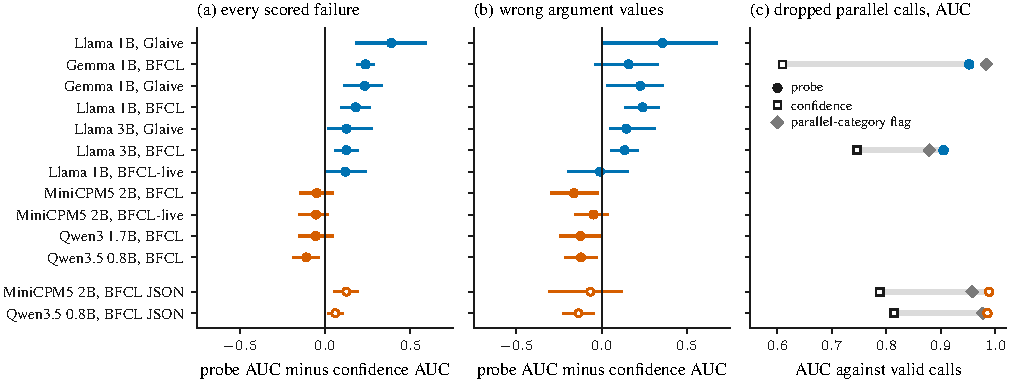
\includegraphics{fig1_types}
\caption{(a) Token-role probe AUC minus mean log-probability AUC on held-out tools, every scored failure against valid calls, dot at the mean over five split seeds, bar the 95\% interval from resampling tools. (b) The same on wrong argument values against valid calls, for runs with at least twenty of them. (c) AUC of the probe (dot), the mean log-probability (open square) and a one-bit flag for a request in a parallel category (grey diamond) on dropped parallel calls against valid calls, for runs with at least twenty dropped calls. Blue Llama-3.2 and Gemma-3, orange Qwen3, Qwen3.5 and MiniCPM5, open markers the forced-JSON runs.}
\label{fig:types}
\end{figure*}

A language model agent acts by calling tools. When it calls the wrong tool, or the right one with wrong arguments, the call is usually well formed, so the runtime executes it before anyone reads the transcript. A guardrail therefore has to judge the call between its generation and its execution. Two signals are available there. The output distribution gives the probability of each generated token, which every serving stack returns. The hidden states give a probe something to read, which only a stack that runs the model's own code can expose.

Probes on the residual stream separate wrong calls from right ones with high accuracy \citep{healy2026internal,yeats2026calls}, and \citet{ke2026neurons} separate three failures, invalid arguments, unneeded calls and missing calls, and detect each from a few neurons. \wscitet{} compared token probabilities with probes on tool calls under splits by prompt. What these studies do not report is which wrong calls the model's own token probabilities miss on tools absent from training, and whether a judge that reads only the output text would catch them. That is the question this paper answers.

We answer it with one quantity, the internal advantage: the area under the curve (AUC) of a probe on the residual stream minus that of the mean token log-probability of the call, on tools never seen in training, beside a floor that reads only lengths. We compute it on every scored failure and on each kind of error against valid calls, and we set the probe against two trained comparators that need no access to the deployed model's states: an output-only judge fitted on the same labels and a second small language model that reads the request and the call.

The main result is the value-error split (\cref{fig:types}b). On wrong argument values the probe leads confidence on \nWavInternalsPos{} of the \nInternalsRuns{} Llama-3.2 and Gemma-3 runs, by \wavInternalsMin{} to \wavInternalsMax{} (point estimates, intervals excluding zero on \nWavInternalsCiExcl{}). Confidence leads the probe on all \nWavConfidenceRuns{} Qwen3, Qwen3.5 and MiniCPM5 runs, native or forced into JSON, with intervals excluding zero on \nWavConfidenceCiBelow{}. The two sides are assigned by family and hold \nCkptInternals{} checkpoints each, so the split describes these checkpoints and is not a test. Much of the probe's lead on value errors is readable from the output: the output-only judge recovers at least half of it on \nJwShareMajority{} of the \nJwEligible{} probe-side runs where the probe leads, and none of it on either Llama-3.2-3B run.

In practice this gives an order of operations (\cref{sec:discussion}): score the model's confidence on its value errors on held-out tools first, where it misses them train a judge on the output text and compare it with a probe before choosing, and for parallel requests count the calls, since a one-bit category flag already separates dropped calls on these runs.

\paragraph{Contributions.}
\begin{enumerate}[topsep=1pt,itemsep=1pt,leftmargin=1.3em]
\item The value-error split, measured on \nRunsPowered{} powered runs from \nCkpt{} checkpoints of four developers on held-out tools, with a length floor and a paired interval on every difference (\cref{sec:result}). This paper adds the decomposition by kind of error against the model's own confidence on held-out tools. \citet{ke2026neurons} split failures into validity, over-calling and missing calls for internal detectors, without the model's confidence beside them.
\item The comparators that bound the claim: an output-only judge and a reader model under the probe's protocol, on every scored failure and on value errors, which show on which runs the probe's lead is readable from the text (\cref{sec:judges}).
\item The controls and the disclosures that condition the split: item difficulty, label budget, the confidence summary, duplicated Glaive requests, the prompt route, extraction provenance, and a dropped-call contrast that a one-bit category flag matches (\cref{sec:result,sec:controls}).
\end{enumerate}

\section{Related work}
\label{sec:related}

\paragraph{Probes on hidden states.}
Supervised probes on the residual stream recover whether a statement is true \citep{azaria2023internal,marks2024geometry}, predict hallucination risk from the query alone \citep{ji2024internal} and stand in for sampling-based uncertainty at the cost of one pass \citep{kossen2024sep}. \citet{orgad2025know} locate the signal at the exact-answer tokens, which is the observation the token-role probe of \citet{healy2026internal} applies to a call's name, arguments and closing delimiter. \citet{yeats2026calls} train linear probes on eighteen models on BFCL and find that model size predicts probe accuracy first and probing depth second. \citet{ke2026neurons} find small sets of neurons that detect invalid arguments, unneeded calls and missing calls on six models. These results establish that internal detectors of wrong calls work. \citet{healy2026internal} and \citet{yeats2026calls} hold out items, so a tool seen in training can return at test, and neither reports the model's own token probabilities on the same items.

\paragraph{Token probabilities against probes on tool calls.}
\wscitet{} compared the mean token log-probability with the token-role probe and with head-averaged spectral probes on Glaive under splits by prompt, and asked whether the best detector changes with model scale. They found token probabilities near chance and head-averaged spectra strong. Under the tool-held-out splits and the repaired labels of \cref{sec:setup}, neither finding holds (\cref{sec:result,sec:attention}): confidence ranges from \confMinPowered{} to \confMaxPowered{} AUC, head-averaged readouts sit near the length floor, and the side a model falls on does not change from Llama-3.2-1B to 3B. This paper adds the decomposition by kind of error, the output-only comparators and three further families.

\paragraph{Readouts of attention.}
LapEigvals trains a probe on the top eigenvalues of the attention Laplacian \citep{binkowski2025lapeigvals}, Lookback Lens on the share of attention paid to the context \citep{chuang2024lookback}, LLM-Check on eigenvalues of attention kernels \citep{sriramanan2024llmcheck} and SinkProbe on attention sinks \citep{binkowski2026sinks}. \citet{noel2025gsp} introduced graph-signal diagnostics on the Laplacian of a head-averaged attention graph, and \citet{dahlem2026transport} prove that every transpose-invariant spectral diagnostic is blind to the direction of attention flow. We reimplement LapEigvals, Lookback Lens and SinkProbe after their authors' papers and code, and score them under the probe's classifier, floor and held-out tools. No numerical parity check against the original implementations is reported, so their numbers here are those of our reimplementations.

\paragraph{Output confidence.}
Token probabilities are informative about a model's own correctness on question answering \citep{kadavath2022know}, and sampling-based estimates sharpen them \citep{farquhar2024semantic,manakul2023selfcheckgpt} at a cost in forward passes that an agent about to act does not have. Tool-calling benchmarks measure whether a call is right \citep{patil2025bfcl,patil2024gorilla,qin2024toolllm} and not whether the model's confidence tracks it. Our contribution is to put the single-pass confidence of the model beside single-pass judges on its internals and on its output, per kind of error, on unseen tools.

\section{Setup}
\label{sec:setup}

\paragraph{Task, labels and kinds of error.}
A model receives a user request and a set of tool schemas and generates greedily. The call is parsed in whichever format the model writes and compared with the benchmark's ground truth after both are normalised to a name and an argument dictionary. Each call receives one failure mode: valid, wrong name, wrong argument values, missing arguments, missing parallel calls, an unneeded call, no call, an unparseable call, or a call cut off by the budget. Every number is computed on the scored population, the items where a call is required and the generation can be judged, and "every scored failure" means every failure mode in that population. We also score two kinds of error against the valid calls alone: wrong argument values, where the right tool gets a wrong value, and dropped parallel calls, where a request needs several calls and the model writes fewer.

\paragraph{Prompt route.}
Tool schemas reach the model through its own chat template where the template carries them. Gemma-3's template drops the tool argument, so every Gemma-3 run, and both forced-JSON runs, use a fallback system prompt that lists the schemas and asks the model to reply with only one JSON object of the form name and arguments and nothing else (\cref{app:protocol}). Rendering one prompt per model on CPU with the paper's render function confirms that Gemma-3 is the only one of the six whose template drops the schemas. A prompt that asks for one object invites a model to drop the other calls of a parallel request, so dropped calls on these runs are partly a property of the prompt, and \cref{sec:result} treats them that way.

\paragraph{Conditioning facts.}
The labelling and extraction code was audited and repaired before the measurements here (\cref{app:audit}). The largest repair concerns correct list-valued arguments, which had been scored wrong on the JSON formats: on Qwen3-1.7B it turned \repPosBeforeQwenThreeBfcl{} labelled failures into \repPosAfterQwenThreeBfcl{}. Relabelling the stored generations of \nRelabelRuns{} runs with the released labeller reproduces every stored label. Two extractor generations coexist (\cref{tab:provenance}): \nFirstExtractInternals{} of the \nInternalsRuns{} probe-side runs and \nFirstExtractConfidence{} of the \nConfidenceRuns{} confidence-side runs keep the first extraction, which records no commit, and the re-extracted runs do not all come from a clean tree. One run extracted under both reads \replGapStale{} and \replGapClean{}, a drift of \replGapDelta{}. Some failures are schema echoes, calls whose arguments copy the tool's JSON schema: a pattern for a copied \texttt{properties} field or object type finds them in \echoPosGemmaBfcl{}\% of Gemma-3 failures on BFCL and on no confidence-side run. Most are labelled missing arguments and stay out of the value-error comparison.

\paragraph{Models and benchmarks.}
The checkpoints are Llama-3.2-1B and 3B, Gemma-3-1B, Qwen3-1.7B, Qwen3.5-0.8B and MiniCPM5-2B, from four developers, released between September 2024 and September 2026 (\cref{app:models}). The chat templates of the Qwen3, Qwen3.5 and MiniCPM5 checkpoints carry a reasoning mode, which is disabled at generation throughout. The benchmarks are the Glaive function-calling corpus \citep{glaive2024}, the single-turn categories of BFCL-v4 \citep{patil2025bfcl} and its live categories, contributed by users. Glaive repeats requests: on Llama-3.2-1B its \gdNScoredLlamaOneBGlaive{} scored items hold \gdNUniquePromptsLlamaOneBGlaive{} unique requests. A run is one checkpoint on one benchmark. A run with fewer than thirty items of either class is underpowered and excluded from every aggregate, which leaves the confidence-side checkpoints with powered runs on BFCL and BFCL-live only. A kind of error is scored on a run only with at least twenty failures of that kind.

\paragraph{Detectors.}
Confidence is the mean token log-probability over the generated call, with its direction fixed on training items, chosen before any result was seen. It averages over every token of the call, while the probe reads the name, the argument values and the delimiter separately. The probe is the token-role probe of \citet{healy2026internal}, a regularised logistic regression on the residual state at the function name, the mean over argument-value tokens and the closing delimiter, at eight depths. The output-only judge is one logistic regression on what an operator sees from outside the model: lengths, benchmark category, counts read off the call, every stored confidence summary, and character n-grams of the call and the request. The reader is Qwen3.5-0.8B, which reads the request and the call as plain text, without schemas, and is probed with the same classifier. It is the same checkpoint as one confidence-side model. The floor is a classifier on prompt length, generation length and truncation.

\paragraph{Protocol and the two sides.}
Items are grouped by ground-truth tool and split five ways at the group level, so every score is on tools absent from training. Every trained detector is fitted on the training folds restricted to the scored population, with a validation carve-out of training tools. One pooled AUC is computed per split seed, and five seeds are averaged. Every difference between detectors is a paired bootstrap that resamples whole tools, with its 95\% percentile interval. The internal advantage of a run is the AUC of the probe minus that of confidence. Each run is assigned to a side by its family, fixed in the analysis code when the split was first described: Llama-3.2 and Gemma-3 on the probe side, Qwen3, Qwen3.5 and MiniCPM5 on the confidence side. The assignment came from the data it describes, and a run can disagree with its side.

\section{The internal advantage by kind of error}
\label{sec:result}

\begin{table*}[t]
\centering
\footnotesize
\setlength{\tabcolsep}{1.5pt}
\caption{Every run under the corrected labels. $n_+$ and $n_-$ are the labelled failures and valid calls in the scored population. The AUC columns are the length floor, the mean log-probability (conf.), the output-only judge, the Qwen3.5-0.8B reader and the token-role probe, all on every scored failure. The last four columns are differences of AUC on held-out tools: probe minus confidence on every scored failure with its 95\% tool-resampled interval, probe minus the output-only judge on every scored failure, and probe minus confidence on wrong argument values and on dropped parallel calls within the parallel categories, each against valid calls. $^{\circ}$ the interval excludes zero (intervals in \cref{app:judges,app:types}). n.c.\ not computed: too few failures of that kind or of valid parallel calls, an underpowered run, or a comparator not fitted on that run. $^{*}$ re-extracted under the corrected extractor. $^\dagger$ fewer than thirty items of one class.}
\label{tab:main}
\begin{tabular}{@{}llrrccccccccc@{}}
\toprule
Model & Data & $n_+$ & $n_-$ & floor & conf. & judge & reader & probe & probe $-$ conf. & probe $-$ judge & value err. & dropped \\
\midrule
Llama-3.2-1B & Glaive & 221 & 359 & 0.539 & 0.576 & 0.910 & 0.949 & 0.963 & $+0.387$ {\scriptsize$[+0.18, +0.59]$} & $+0.053^{\phantom{\circ}}$ & $+0.357^{\circ}$ & n.c. \\
Llama-3.2-1B$^{*}$ & BFCL & 161 & 339 & 0.635 & 0.651 & 0.755 & 0.818 & 0.831 & $+0.180$ {\scriptsize$[+0.09, +0.27]$} & $+0.077^{\circ}$ & $+0.240^{\circ}$ & n.c. \\
Llama-3.2-1B & BFCL-live & 208 & 157 & 0.709 & 0.663 & 0.682 & 0.795 & 0.782 & $+0.119$ {\scriptsize$[-0.00, +0.24]$} & $+0.101^{\circ}$ & $-0.010^{\phantom{\circ}}$ & n.c. \\
Llama-3.2-3B & Glaive & 90 & 555 & 0.522 & 0.785 & 0.684 & 0.931 & 0.911 & $+0.126$ {\scriptsize$[+0.02, +0.28]$} & $+0.227^{\phantom{\circ}}$ & $+0.145^{\circ}$ & n.c. \\
Llama-3.2-3B & BFCL & 120 & 576 & 0.618 & 0.707 & 0.633 & 0.758 & 0.831 & $+0.125$ {\scriptsize$[+0.05, +0.20]$} & $+0.199^{\circ}$ & $+0.134^{\circ}$ & $+0.158^{\circ}$ \\
Gemma-3-1B & Glaive & 158 & 460 & 0.704 & 0.650 & 0.872 & 0.853 & 0.883 & $+0.233$ {\scriptsize$[+0.11, +0.34]$} & $+0.011^{\phantom{\circ}}$ & $+0.226^{\circ}$ & n.c. \\
Gemma-3-1B$^{*}$ & BFCL & 364 & 150 & 0.842 & 0.711 & 0.900 & 0.927 & 0.948 & $+0.237$ {\scriptsize$[+0.19, +0.29]$} & $+0.048^{\circ}$ & $+0.158^{\phantom{\circ}}$ & $+0.342^{\circ}$ \\
\midrule
Qwen3-1.7B & BFCL & 52 & 639 & 0.628 & 0.799 & 0.558 & 0.662 & 0.745 & $-0.053$ {\scriptsize$[-0.16, +0.05]$} & $+0.187^{\circ}$ & $-0.124^{\phantom{\circ}}$ & n.c. \\
Qwen3-1.7B$^\dagger$$^{*}$ & Glaive & 10 & 699 & 0.677 & 0.867 & n.c. & n.c. & 0.676 & $-0.191$ {\scriptsize$[-0.65, +0.21]$} & n.c. & n.c. & n.c. \\
MiniCPM5-2B$^{*}$ & BFCL & 54 & 640 & 0.578 & 0.823 & 0.585 & 0.677 & 0.775 & $-0.048$ {\scriptsize$[-0.15, +0.05]$} & $+0.190^{\circ}$ & $-0.162^{\circ}$ & n.c. \\
MiniCPM5-2B$^{*}$ & BFCL-live & 120 & 475 & 0.545 & 0.797 & 0.642 & 0.655 & 0.744 & $-0.053$ {\scriptsize$[-0.15, +0.02]$} & $+0.102^{\circ}$ & $-0.048^{\phantom{\circ}}$ & n.c. \\
MiniCPM5-2B$^\dagger$$^{*}$ & Glaive & 9 & 716 & 0.685 & 0.913 & n.c. & n.c. & 0.710 & $-0.203$ {\scriptsize$[-0.51, +0.01]$} & n.c. & n.c. & n.c. \\
Qwen3.5-0.8B$^{*}$ & BFCL & 86 & 398 & 0.601 & 0.792 & 0.678 & 0.730 & 0.682 & $-0.110$ {\scriptsize$[-0.19, -0.03]$} & $+0.004^{\phantom{\circ}}$ & $-0.121^{\circ}$ & n.c. \\
\midrule
MiniCPM5-2B$^{*}$ & BFCL, JSON & 83 & 514 & n.c. & 0.757 & n.c. & n.c. & 0.882 & $+0.125$ {\scriptsize$[+0.05, +0.19]$} & n.c. & $-0.066^{\phantom{\circ}}$ & $+0.201^{\circ}$ \\
Qwen3.5-0.8B$^{*}$ & BFCL, JSON & 226 & 436 & n.c. & 0.808 & n.c. & n.c. & 0.868 & $+0.060$ {\scriptsize$[+0.01, +0.11]$} & n.c. & $-0.136^{\circ}$ & $+0.171^{\circ}$ \\
\bottomrule
\end{tabular}

\end{table*}

On every scored failure, the \nRunsInternals{} powered Llama-3.2 and Gemma-3 runs have an internal advantage of \gapInternalsMin{} to \gapInternalsMax{}, with an interval excluding zero on \nInternalsCiExcludesZero{} of them (\cref{tab:main}, \cref{fig:types}a). The \nRunsConfidence{} powered Qwen3, Qwen3.5 and MiniCPM5 runs read \gapConfidenceMin{} to \gapConfidenceMax{}, with an interval below zero on \nConfidenceCiBelowZero{}. Runs that share a checkpoint are not independent. With \nCkptInternals{} against \nCkptConfidence{} checkpoints the smallest attainable two-sided rank-test value is $p=\ckptExactFloor{}$, so the separation is a description of these \nCkpt{} checkpoints.

\paragraph{Wrong argument values.}
Every scored failure mixes kinds of error, so \cref{fig:types}b scores wrong argument values against valid calls alone. The probe leads confidence on \nWavInternalsPos{} of the \nInternalsRuns{} probe-side runs, by \wavInternalsMin{} to \wavInternalsMax{} in point estimate, with an interval excluding zero on \nWavInternalsCiExcl{}. The largest lead, Llama-3.2-1B on Glaive, has the widest interval, [\WavGapLoLlamaOneBGlaive{}, \WavGapHiLlamaOneBGlaive{}]. Llama-3.2-1B on the live categories reads \WavGapLlamaOneBLive{}, on the probe side by family and on neither side by measurement. Confidence leads the probe on all \nWavConfidenceRuns{} confidence-side runs, native and forced into JSON, where the advantage is \wavConfidenceMin{} to \wavConfidenceMax{}, with an interval excluding zero on \nWavConfidenceCiBelow{}. On these models the mean log-probability ranks most wrong values below right ones. Glaive repeats requests, and keeping the first occurrence of each unique request leaves the value-error advantage at \gdWavLlamaOneBGlaive{} on Llama-3.2-1B and \gdWavGemmaGlaive{} on Gemma-3.

\paragraph{Dropped parallel calls.}
A one-bit flag for a request in a parallel category separates dropped calls from valid calls at \catAucMin{} to \catAucMax{} AUC on the four runs with at least twenty of them (\cref{fig:types}c), because only parallel requests can drop a call. On Gemma-3 the flag reaches \catAucGemmaBfcl{} against the probe's \catProbeGemmaBfcl{}. Three of these runs use the fallback prompt that asks for one JSON object. Within the parallel categories, where the flag is constant, the probe leads confidence on MiniCPM5-2B and Qwen3.5-0.8B under forced JSON, \PwGapMiniCpmBfclJson{} [\PwGapLoMiniCpmBfclJson{}, \PwGapHiMiniCpmBfclJson{}] and \PwGapQwenThreeFiveBfclJson{} [\PwGapLoQwenThreeFiveBfclJson{}, \PwGapHiQwenThreeFiveBfclJson{}]. On Llama-3.2-3B, the only one of the four prompted through its native template, the lead vanishes at \PwGapLlamaThreeBBfcl{} [\PwGapLoLlamaThreeBBfcl{}, \PwGapHiLlamaThreeBBfcl{}], and Gemma-3 makes too few valid parallel calls to be tested. No claim about dropped calls is made beyond these three numbers.

\paragraph{Output format and R3.}
Qwen3 writes JSON like Llama-3.2 and Gemma-3 and sits on the confidence side, so the native format does not decide the side. Registered prediction R3 said that, forced to write JSON, the confidence-side families keep an advantage at or below zero on every scored failure, and that it fails above \rThreeThreshold{}. It failed on MiniCPM5-2B, at \rThreeJsonMiniCpm{} [\rThreeJsonLoMiniCpm{}, \rThreeJsonHiMiniCpm{}], on a partial run of \nJsonItemsMiniCpm{} of \nAllMiniCpmBfcl{} items extracted from a tree with uncommitted changes. On Qwen3.5-0.8B it is undecided by the rule, at \rThreeJsonQwenThreeFive{} [\rThreeJsonLoQwenThreeFive{}, \rThreeJsonHiQwenThreeFive{}]. Dropped parallel calls make up \rThreeMcJsonMiniCpm{} of \rThreePosJsonMiniCpm{} and \rThreeMcJsonQwenThreeFive{} of \rThreePosJsonQwenThreeFive{} failures under the fallback prompt, against \rThreeMcNatMiniCpm{} and \rThreeMcNatQwenThreeFive{} under the native templates. On wrong argument values both models stay on the confidence side.

\paragraph{Size and release date.}
Size does not separate the sides (one and three billion parameters against 0.8 to two), and within Llama-3.2 the probe does not improve from 1B to 3B (\aucProbeLlamaOneBBfcl{} at both sizes on BFCL). Release date, a reasoning mode and native tool-calling post-training all separate the six checkpoints (\cref{sec:discussion}).

\paragraph{Calls with a history.}
One multi-turn run, MiniCPM5-2B, reads \mtAucProbe{} for the probe and \mtAucConf{} for confidence, the opposite order to its single-turn runs, on \mtGroupsAll{} linked groups. It is anecdotal and enters no claim (\cref{app:multiturn}).

\section{What the probe adds over the output text}
\label{sec:judges}

\begin{figure*}[t]
\centering
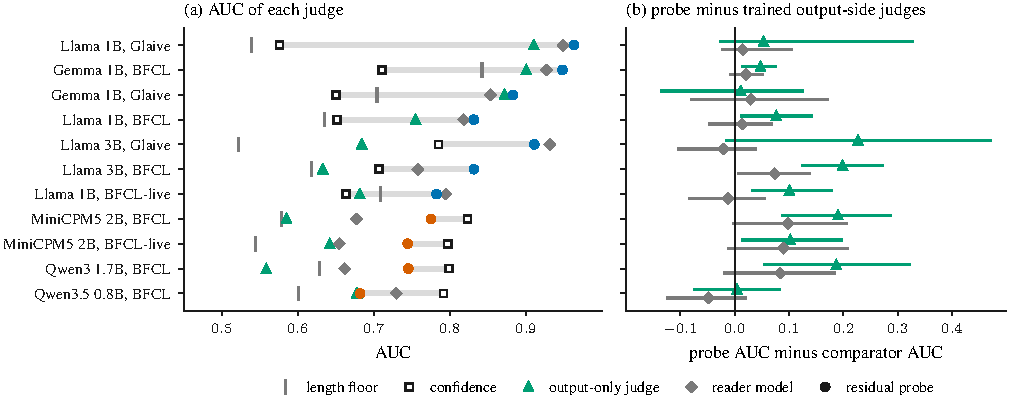
\includegraphics{fig2_judges}
\caption{(a) AUC per powered run of the length floor, the mean log-probability, the output-only judge, the \readerName{} reader and the token-role probe, with the span from confidence to probe shaded. (b) Probe AUC minus output-only judge AUC (triangles) and minus reader AUC (diamonds), with 95\% tool-resampled intervals. Reader points appear on the runs where the reader was fitted.}
\label{fig:judges}
\end{figure*}

The internal advantage sets a trained probe against an untrained summary of the output, so part of the probe's lead could come from training on labels rather than from the hidden states. The comparators of this section are trained on the same labels, folds and training population as the probe and read only what is visible outside the deployed model.

\paragraph{The output-only judge.}
On the confidence side the output-only judge scores \ojMinConfidence{} to \ojMaxConfidence{}, below confidence itself, because a few dozen failures cannot fit its n-gram features. On the probe side it is strong (\cref{fig:judges}a). It recovers \ojShareMajorityMin{} to \ojShareMajorityMax{}\% of the probe's lead over confidence on \nOjShareMajority{} of the \nInternalsRuns{} runs, all of them Llama-3.2-1B or Gemma-3 runs. Probe minus output-only judge is \ojGapMinInternals{} to \ojGapMaxInternals{} and excludes zero on \nOjGapCiExcl{} runs, against \nGapCiExcl{} for probe minus confidence. On Gemma-3 on BFCL the judge reaches \aucOutJudgeGemmaBfcl{} against the probe's \aucProbeGemmaBfcl{}, and a structural floor that counts schema keywords already reaches \aucStructGemmaBfcl{}. On Llama-3.2-3B the judge trails the probe by \GapOutJudgeLlamaThreeBGlaive{} on Glaive and \GapOutJudgeLlamaThreeBBfcl{} on BFCL.

\paragraph{A second model reading the call.}
A reader that is a different language model, given the request and the generated call as plain text, is a stronger output-side judge than n-grams. On the \nReaderInternals{} probe-side runs, probe minus reader ranges from \readerGapMinInternals{} to \readerGapMaxInternals{}, and its interval contains zero on \nReaderTiesInternals{} of them (\cref{fig:judges}b). On all three Llama-3.2-1B runs and on Llama-3.2-3B on Glaive the reader is within two points of the model's own probe (\cref{tab:main}). The one run where the probe beats every output-side judge is Llama-3.2-3B on BFCL, by \GapReaderLlamaThreeBBfcl{} [\GapReaderLoLlamaThreeBBfcl{}, \GapReaderHiLlamaThreeBBfcl{}] over the reader. On the other probe-side runs the probe shows that the error is visible in the call. The claim that the model's states hold what its confidence lacks, beyond what its text shows, rests on that one run. On the confidence side the reader scores \readerMinConfidence{} to \readerMaxConfidence{}, below the model's own confidence with an interval excluding zero on \nReaderBelowConf{} of the \nConfidenceRuns{} runs.

\paragraph{What the probe adds.}
Fusing the probe with the output-only judge by an equal-weight rank average, with no fitted weight, gains \fusOutMinInternals{} to \fusOutMaxInternals{} over the judge alone on the probe side, with an interval excluding zero on \nFusOutCiExclInternals{} of \nInternalsRuns{} runs. The value-error split itself does not depend on any of these comparators, because it compares the probe with the model's own confidence on one kind of error.

\section{Controls on the split}
\label{sec:controls}

\begin{figure*}[t]
\centering
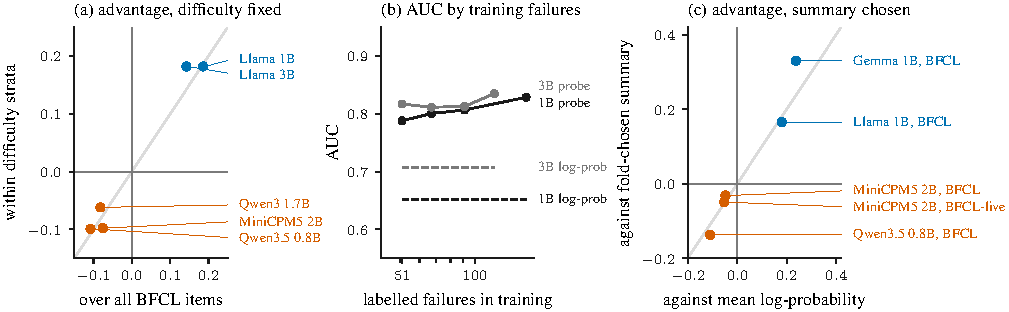
\includegraphics{fig3_controls}
\caption{(a) Internal advantage within strata of item difficulty against the advantage over all BFCL items, one point per checkpoint, identity line grey. Difficulty is the share of the other checkpoints that fail the item. (b) Token-role probe AUC (solid) and mean log-probability AUC (dashed) against the labelled failures available for training on Llama-3.2-1B and 3B, log scale. (c) Internal advantage against a confidence summary chosen on training folds and against the mean log-probability, one point per run that stores several summaries, identity line grey.}
\label{fig:controls}
\end{figure*}

A difference between model families can come from the items, the labels or the protocol. Each paragraph below changes one thing and keeps the rest of the protocol fixed.

\paragraph{Item difficulty.}
A model that fails rarely fails on hard items, and its confidence may register hardness instead of its own error. On BFCL an item's difficulty is the share of the other checkpoints that fail it. That share alone predicts a model's failures at \diffOnlyMin{} to \diffOnlyMax{} AUC. Scoring both detectors inside strata of difficulty removes what either gains from knowing which items are hard, and the split does not close (\cref{fig:controls}a). The advantage is \diffGapWithinLlamaOneB{} on Llama-3.2-1B and \diffGapWithinLlamaThreeB{} on Llama-3.2-3B, and between \diffGapWithinQwenThreeFive{} and \diffGapWithinQwenThree{} on the three confidence-side checkpoints. Confidence on the confidence side tracks the model's own errors beyond the hardness of the request.

\paragraph{Label budget.}
A probe needs labelled failures and confidence needs none, and the confidence-side models fail less often. Training the Llama-3.2 probes on as few failures as the other families supply, with the test folds untouched, costs them \budgetProbeDropLlamaOneB{} AUC at 1B and \budgetProbeDropLlamaThreeB{} at 3B (\cref{fig:controls}b). At \budgetMinPosLlamaOneB{} training failures the advantage is still \budgetGapAtMinLlamaOneB{} and \budgetGapAtMinLlamaThreeB{}, above every value on the other side.

\paragraph{The confidence summary.}
The mean log-probability is one summary of the output distribution. On the runs that store up to \nSummariesLlamaOneBBfcl{} length-invariant summaries, the summary with the highest AUC on the other folds is applied fold by fold, so no summary is chosen on the items it scores (\cref{fig:controls}c, \cref{app:confidence}). The advantage becomes \gapBestLlamaOneBBfcl{} on Llama-3.2-1B and \gapBestGemmaBfcl{} on Gemma-3 on BFCL, and at most \gapBestConfidenceMax{} on the confidence side. An oracle that picks the best summary on the test items leaves the probe side at \gapOracleMinInternals{} or more.

\paragraph{Benchmark and schema echoes.}
Gemma-3 reads \GapGemmaGlaive{} on Glaive and \GapGemmaBfcl{} on BFCL, Llama-3.2-1B keeps its side on three benchmarks and MiniCPM5 on two, so no run's side depends on its benchmark. With matched schema echoes removed from evaluation, the pooled advantage keeps its sign on \nNoEchoHolds{} of the \nInternalsRuns{} probe-side runs. The exception is Llama-3.2-1B on the live categories, which moves from \GapLlamaOneBLive{} to \GapNoEchoLlamaOneBLive{} [\GapNoEchoLoLlamaOneBLive{}, \GapNoEchoHiLlamaOneBLive{}]. Its value-error advantage is also near zero, so this run is on neither side once format failures are set aside.

\paragraph{Chance level of the pipeline.}
With the labels permuted, \nullN{} refits of the whole probe pipeline on Qwen3.5-0.8B score \nullMean{} AUC with a standard deviation of \nullSd{}. The standard deviation of the permuted advantage is \nullGapSd{}, which is why single-run advantages of a few hundredths are not interpreted. Inside individual folds the advantage is negative on \foldNegMinInternals{} to \foldNegMaxInternals{} of \nFoldGaps{} fold and seed pairs on the probe side and on \foldNegMinConfidence{} to \foldNegMaxConfidence{} on the confidence side.

\paragraph{Training population and pooling.}
Training the probe on the scored population only, and fixing the sign of the log-probability on that population, both moved the numbers toward confidence (\cref{app:audit}). Pooling out-of-fold scores across folds penalises a fitted probe and not a fixed score: the advantage computed within folds exceeds the pooled one by \poolShiftMean{} on average.

\section{Attention readouts, head averaging and cost}
\label{sec:attention}

\begin{figure*}[t]
\centering
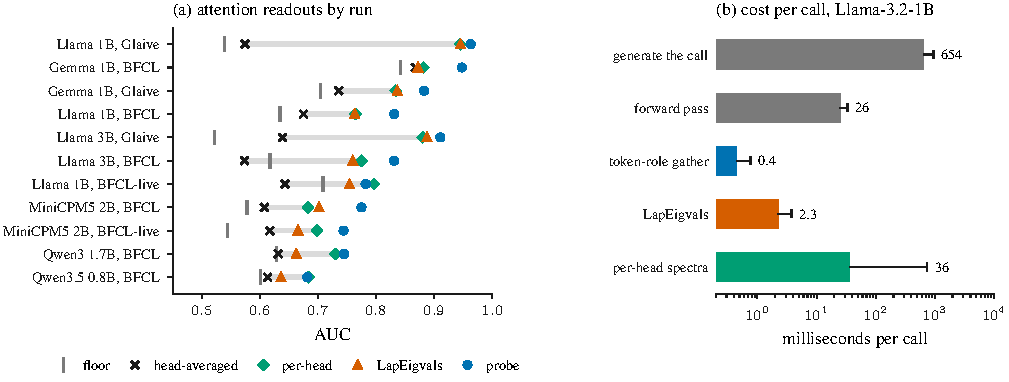
\includegraphics{fig4_attention}
\caption{(a) AUC per powered run, every scored failure, of the length floor, the head-averaged spectral profile, the per-head spectral profile, LapEigvals and the token-role probe, with the span from head-averaged to per-head shaded. (b) Cost per call of each path on Llama-3.2-1B, bar at the median over \latNPrompts{} BFCL prompts, line to the 90th percentile, log scale, one consumer GPU.}
\label{fig:attention}
\end{figure*}

A stack may expose attention weights but not activations. Three readouts of the attention on the generated call are compared here. The per-head spectral profile takes each head's attention on the call, symmetrises it into a graph and keeps five eigenvalue statistics of its normalised Laplacian per head and layer. The head-averaged profile computes the same statistics on the graph averaged over heads, which is how most of this literature reads a layer. The anchored readout keeps the attention rows of the call's own tokens per head, without a spectrum.

On the probe-side runs the per-head profile and LapEigvals trail the token-role probe by a few points (\cref{fig:attention}a), for instance \GapProbePerHeadLlamaOneBBfcl{} on Llama-3.2-1B and \GapProbePerHeadGemmaBfcl{} on Gemma-3 on BFCL. The two are within noise of each other, and on Llama-3.2-1B and Gemma-3 on BFCL, the two runs where it was computed, the anchored readout ties the per-head profile (\GapAnchPerHeadLlamaOneBBfcl{} and \GapAnchPerHeadGemmaBfcl{}).

\paragraph{Head averaging.}
The head-averaged profile sits within \havgFloorMinInternals{} to \havgFloorMaxInternals{} of the length floor on the probe-side runs. Keeping heads apart gains \ladGainPerHead{} on average over \ladNRuns{} runs, and permuting the head axis per item, which keeps every value and destroys only which head produced it, costs \ladGainVsShuffle{} (\cref{app:ladder,app:proofs}).

\paragraph{Cost.}
Reading confidence costs nothing beyond generation. Every internal judge needs a teacher-forced pass over prompt and call, \latPass{}\,ms against \latGen{}\,ms of generation (\cref{fig:attention}b). On top of the pass the token-role features cost \latTokenRole{}\,ms and LapEigvals \latLapEig{}\,ms, and the per-head spectra \latPerHead{}\,ms at the median and \latPerHeadNinety{}\,ms at the 90th percentile. The output-only judge needs no pass of the deployed model, and the reader one pass of Qwen3.5-0.8B over the request and the call.

\section{Discussion}
\label{sec:discussion}

\paragraph{Readings of the split.}
Two properties of the model set fit all six checkpoints (\cref{tab:models}). One is release date, with a cutoff between March and April 2025. The other, registered as hypothesis H1 before any new model was extracted (\cref{app:registry}), is the post-training recipe: the three confidence-side families ship a chat template with a reasoning mode and were post-trained with it, and the two probe-side families do not. We read the split as possibly a post-training effect: training that rewards a model for working through a call before writing it may also leave its token probabilities tracking its own value errors. The reading is untested here. Switching the reasoning mode on at generation within Qwen3-1.7B yields \thinkPos{} failures in \thinkScored{} scored calls, too few to score, and Qwen3 is already on the confidence side with the mode off.
% ---------------------------------------------------------------------------------------------
% WITHIN-MODEL SWAP RESULT GOES HERE (docs/REGISTRATION_SWAP.md, Qwen3.5-4B-Base against Qwen3.5-4B,
% registered 2026-10-04). Only once both arms have been extracted from a committed tree and evaluated:
% one sentence with D and D_wav and their joint tool-bootstrap intervals (macros from the swap's result
% file through analysis/icml_v2_numbers.py), the verdict under the registered rule (PASS, FAIL,
% INCONCLUSIVE or NOT IDENTIFIED), the side of each arm, and the J qualifier. Then rewrite the sentence
% "The reading is untested here" to match the verdict, and add the row to the registry in appendix.tex.
% Nothing about the swap is printed before that result exists.
% ---------------------------------------------------------------------------------------------
A third reading, that a model which has seen the benchmark in training fails less and knows when it fails, is weakened by the live categories, contributed by users after the curated set, on which MiniCPM5 stays on the confidence side.

\paragraph{What confidence misses.}
On the probe side the mean log-probability ranks wrong values close to chance on BFCL, \aucConfWavLlamaOneBBfcl{} on Llama-3.2-1B and \aucConfWavGemmaBfcl{} on Gemma-3, while the residual stream separates them. We interpret this as an output distribution that does not express what the model's states, and on most runs its own text, carry. \cref{sec:judges} bounds the reading.

\paragraph{For operators.}
The decision that changes is which judge to build, if any, in order of cost.

\begin{tcolorbox}[colback=white,colframe=black!60,boxrule=0.5pt,arc=1pt,left=4pt,right=4pt,top=3pt,bottom=3pt,title=\small Before building an internal judge for a tool-calling model]
\small
\begin{enumerate}[topsep=0pt,itemsep=1pt,leftmargin=1.2em]
\item Score the mean token log-probability per kind of error on a few hundred labelled calls from the model to be deployed, on tools absent from the labelled set. Where it already ranks value errors (\cref{tab:main}, confidence side), a probe fused with it gained at most \fusConfMaxConfidence{} AUC over every failure.
\item Where it misses value errors, train an output-only judge or a small reader model on the same labels before reading internals. The output-only judge recovered \ojShareMajorityMin{} to \ojShareMajorityMax{}\% of the probe's lead on \nOjShareMajority{} of \nInternalsRuns{} probe-side runs and needs no access to the model's states.
\item Check dropped parallel calls separately, by counting the calls a parallel request needs. On every run with at least twenty of them the probe led confidence by \mcGapMin{} or more.
\end{enumerate}
\end{tcolorbox}

\paragraph{For model builders.}
If a release reported the internal advantage per kind of error on held-out tools, an operator could see before deployment whether the model's confidence flags its value errors and its dropped calls.

\paragraph{For detector research.}
Under splits by prompt and pooled labels, \wscitet{} found token probabilities near chance and head-averaged spectra strong. Under splits by tool, with the labels repaired and the errors separated, confidence reaches \confMinPowered{} to \confMaxPowered{} AUC and beats the probe on value errors in \nFamiliesConfidence{} of the five families. A probe's accuracy reported without the model's own confidence, without an output-only judge and without held-out tools can show a strong detector on a model that did not need one.

\section{Conclusion}
\label{sec:conclusion}

Whether a tool-calling model's token probabilities catch its wrong calls depends on the model and on the kind of error. On wrong argument values the probe leads confidence on Llama-3.2 and Gemma-3 and trails it on Qwen3, Qwen3.5 and MiniCPM5, whatever format the latter are made to write. On dropped parallel calls the probe leads wherever there are enough of them. Much of the probe's lead is visible in the text of the call to a judge that never reads the model's internals. Three recommendations follow, in order of cost: score the model's confidence per kind of error on held-out tools before building any judge, train a judge on the output text before a probe where confidence misses value errors, and check dropped parallel calls separately.

\section{Limitations}
\label{sec:limitations}

The first limitation is the instrument. Labels come from comparing a call with a benchmark's ground truth, which is a proxy for whether the action would have been harmful, and \cref{app:audit} shows that a parser can manufacture a family effect. The hand audit after the second repair found \auditPooledErr{} errors in \auditPooledN{} items, all correct calls scored as failures, and the residual after the third repair is unmeasured. Errors of that kind favour probes, so residual label error would move runs toward the probe side.

The second is the design. The sides were assigned by family after the split had been seen, \nCkptInternals{} checkpoints each, so no checkpoint-level test can separate them, and release date, a reasoning mode and native tool-calling post-training all fit the division. The prompt differs by family: Gemma-3 and the forced-JSON runs go through a fallback prompt that asks for one JSON object. The comparator favours the probe, which is trained, over confidence, which is not, and the reader sees no tool schemas, so it understates what the text reveals.

The third is provenance. The first extractor produced \nFirstExtractInternals{} of the \nInternalsRuns{} probe-side runs and \nFirstExtractConfidence{} of the \nConfidenceRuns{} confidence-side runs and recorded no commit, and \nDirtyRuns{} of the re-extracted runs, among them three confidence-side runs, come from a tree with uncommitted changes (\cref{tab:provenance}). A run extracted twice drifted by \replGapDelta{}.

The fourth is scale and realism. Every checkpoint has at most three billion parameters, and \citet{yeats2026calls} find probe accuracy rising with size, so the side a family falls on above this range is open. Calls are single-step on three benchmarks of English requests, the confidence side is powered on two of them, the multi-turn replay is one anecdotal run, and cost is measured on one consumer GPU.


\section*{Impact statement}
This work measures open-weight language models on public tool-calling benchmarks, trains no language model and involves no human subjects. Its aim is defensive: to tell an operator which wrong tool calls a model's own confidence already flags and which ones need another judge before the call executes. The same detectors could guide the construction of calls that evade them, which is why we report every kind of error and every run on which a detector weakens rather than one headline number.

\section*{Reproducibility statement}
Every number in this paper expands from a macro that a released script builds from the result files, and a provenance file records the file, field and run each macro reads. Labels are recomputed from the stored generations at evaluation time, and relabelling the stored generations of \nRelabelRuns{} runs with the released labeller reproduces every stored label. Splits are grouped by ground-truth tool and every interval resamples tools. The extractions themselves are not uniform: \cref{tab:provenance} lists, per run, the extractor generation, the commit and whether the tree had uncommitted changes, and the first-generation runs record none of these. \cref{app:registry} dates each registered prediction against the data that test it. Models and benchmarks are public, and the stored extractions the tables are computed from are released with the code.

\bibliography{references}
\bibliographystyle{icml2026}

\appendix
\onecolumn
% the ICML style file deletes addcontentsline. The appendix list needs it back
\makeatletter
\def\addcontentsline#1#2#3{\addtocontents{#1}{\protect\contentsline{#2}{#3}{\thepage}{}}}
\makeatother
\clearpage
\addtocontents{toc}{\protect\setcounter{tocdepth}{2}}
\makeatletter
\renewcommand*\l@section{\@dottedtocline{1}{0em}{2.0em}}
\renewcommand*\l@subsection{\@dottedtocline{2}{2.0em}{2.8em}}
\makeatother
\renewcommand{\contentsname}{Appendix contents}
{\small\setlength{\parskip}{0pt}\tableofcontents}
\medskip

\section{Head averaging under causal attention}
\label{app:proofs}

Purpose: the two statements behind \cref{sec:attention}, proved for the causal attention of the decoders studied here, and the scope of each.

Fix one layer with $H$ heads and $T$ positions. Head $h$ produces a row-stochastic attention matrix $A_h$, lower triangular under a causal mask. It is symmetrised and stripped of self-loops into $W_h = \tfrac12(A_h + A_h^\top) - \operatorname{diag}(\tfrac12(A_h + A_h^\top))$, with combinatorial Laplacian $L_h = D_h - W_h$ and symmetric normalised Laplacian $\mathcal{L}_h = I - D_h^{-1/2} W_h D_h^{-1/2}$. The head-averaged graph is $\bar W = \frac1H \sum_h W_h$, and $\lambda_2$ is the second-smallest eigenvalue.

\begin{proposition}[head averaging is many-to-one]
\label{prop:annihilation}
Any map of the form $\{W_h\} \mapsto \Phi(\bar W)$ is constant on head configurations sharing the same mean. For every $T \ge 3$ there are two configurations of two causal row-stochastic heads with the same mean whose spreads of per-head connectivity, $\max_h \lambda_2(L_h) - \min_h \lambda_2(L_h)$, differ by $\cos(\pi/T) - \tfrac12$.
\end{proposition}
\begin{proof}
The first claim holds because $\Phi$ factors through $\bar W$. For the second, let $A_P$ be the previous-token head, $A_P[i,i-1] = 1$ for $i \ge 1$ and $A_P[0,0] = 1$, and $A_S$ the sink head, $A_S[i,0] = 1$ for every $i$. Both are causal and row-stochastic, and so is $A_M = \tfrac12(A_P + A_S)$. Symmetrisation and the removal of the diagonal are linear, so $W_M = \tfrac12(W_P + W_S)$, and the configurations $\{A_P, A_S\}$ and $\{A_M, A_M\}$ share the mean graph $W_M$. $W_P$ is the path on $T$ nodes with edge weights $\tfrac12$, whose Laplacian has eigenvalues $1 - \cos(k\pi/T)$, so $\lambda_2(L_P) = 1 - \cos(\pi/T)$. $W_S$ is the star centred on position $0$ with edge weights $\tfrac12$, whose Laplacian has eigenvalues $0$, $\tfrac12$ with multiplicity $T-2$, and $T/2$, so $\lambda_2(L_S) = \tfrac12$ for $T \ge 3$. The spread is $\cos(\pi/T) - \tfrac12$ in the first configuration and zero in the second.
\end{proof}

\begin{proposition}[head averaging overstates combinatorial connectivity]
\label{prop:jensen}
For any heads $W_1, \dots, W_H$, $\lambda_2(\bar L) \ge \frac1H \sum_h \lambda_2(L_h)$, with equality if and only if the heads admit a common Fiedler vector.
\end{proposition}
\begin{proof}
The Laplacian is linear in the adjacency, so $\bar L = \frac1H \sum_h L_h$. By the min-max theorem of Courant and Fischer, $\lambda_2(L) = \min_{x \perp \mathbf 1, \|x\|=1} x^\top L x$ is a pointwise minimum of linear functionals of $L$ and hence concave. If $x^\star$ attains the minimum for $\bar L$ then $\lambda_2(\bar L) = \frac1H \sum_h x^{\star\top} L_h x^\star \ge \frac1H \sum_h \lambda_2(L_h)$, with equality exactly when $x^\star$ is a Fiedler vector of every head \citep{chung1997spectral}.
\end{proof}

\paragraph{Scope.}
Both statements hold for any row-stochastic heads, so the causal decoders here are instances of them, and \cref{prop:annihilation} uses only causal heads. \cref{prop:jensen} covers the combinatorial Laplacian only. The spectral detectors of \cref{sec:attention} use the normalised Laplacian, whose Rayleigh quotient is not linear in $W$, and for it no inequality in either direction holds. In the construction of \cref{prop:annihilation}, computed by \texttt{analysis/v2\_causal\_construction.py}, the normalised connectivity of the averaged graph minus the per-head mean is \ccNormDiffSmall{} at $T=\ccTsmall{}$ and \ccNormDiffLarge{} at $T=\ccTlarge{}$, so the sign of the gap changes with length. Under the combinatorial Laplacian the same difference is \ccCombDiffSmall{} at $T=\ccTsmall{}$ and \ccCombDiffLarge{} at $T=\ccTlarge{}$, as \cref{prop:jensen} requires. On \jensenLayers{} measured layers from three models and three inputs the combinatorial inequality holds without violation, the normalised one fails on \jensenNormViolations{} layers, and the averaged graph reports connectivity a median \jensenRatioMedianPct{}\% above the mean over heads. Neither statement predicts which models fall on which side of the value-error split.

\begin{remark}[LapEigvals reads degrees]
\label{rem:lapeig}
\citet{binkowski2025lapeigvals} observe that for a causal attention matrix the Laplacian $L = D - A$ is lower triangular, so its spectrum is its diagonal $\{d_j - A_{jj}\}$. Their top-$k$ features depend on $A$ only through its column sums and diagonal. The symmetrisation above destroys triangularity, so the per-head profile reads global functionals of the routing. The two families are not two estimates of one object, and what they share is that both keep heads apart.
\end{remark}

\section{Protocol details}
\label{app:protocol}

Purpose: every setting needed to rerun the extraction and the scoring without another paper.

\paragraph{Generation.} Greedy decoding in bfloat16 with deterministic kernels, a budget of 256 new tokens (160 on multi-turn prompts), tool schemas passed through the model's chat template with its reasoning mode disabled, and every end-of-turn id of the template among the stopping ids. The rendered text is tokenised without a second beginning-of-sequence token. Each record stores its budget, library versions and commit.

\paragraph{Features.} Residual states are read at eight depths spaced evenly over the layer count at the function-name token, the mean over argument-value tokens and the closing delimiter, located by aligning the parsed call to token offsets in each dialect. Attention features are reduced inside a forward hook on each attention module, on the subgraph induced on the generated call.

\paragraph{Output-only judge and reader.} The structural features are the floor's three lengths, a one-hot benchmark category, and counts read off the generated call: calls, arguments, characters, digits, quoted strings and schema keywords. The confidence features are every stored summary of the token log-probabilities. The text features are character 2 to 5-gram TF-IDF vectors of the call and of the request. The output-only judge concatenates all three. The reader model \readerName{} reads the request, a newline and the generated call, without the tool schemas, and its residual state at eight depths is read at the last token and averaged over the call's tokens. Both are fitted with the probe's classifier on the probe's folds, training population and validation carve-out, and the folds are asserted equal to the stored ones. As a reverse check the same code recomputes the paper's length floor, which matches the stored floor on every run to within \floorReproMaxDiff{}.

\paragraph{Classifiers and scoring.} Logistic regression with $\ell_2$ penalty, standardised features, class balancing and $C \in \{0.01, 0.1, 1, 10\}$ chosen on a one-fifth validation carve-out of training tools. Five tool-grouped folds, training restricted to the scored population, one pooled AUC per seed over five seeds, mean reported. Differences are paired bootstraps that resample whole tools, 2000 draws per seed for the stored contrasts and 1000 for the audit contrasts, draws pooled over seeds, percentile intervals.

\section{Labelling and extraction defects found by the audit}
\label{app:audit}

Purpose: the repairs that condition every number, with the side each defect favoured.

\begin{center}\small
\begin{tabular}{p{0.38\linewidth}p{0.26\linewidth}p{0.28\linewidth}}
\toprule
Defect & Where it fell & Favoured \\
\midrule
A predicted list argument was collapsed to its first element by the unwrapping meant for ground truth, so correct list-valued calls were scored wrong & JSON formats (Llama-3.2, Qwen3). \repPosBeforeQwenThreeBfcl{}\,$\to$\,\repPosAfterQwenThreeBfcl{} failures on Qwen3-1.7B & probes, through a surface feature \\
Semicolon-separated parallel calls did not parse and were scored unparseable & Llama-3.2-3B, \repParallelLlamaThreeBBfcl{} calls returned to the scored population & probes \\
A list sent as a string was compared inconsistently with a list & Llama-3.2 & probes \\
Probe positions never located in the MiniCPM5 dialect, so the probe read the end-of-sequence state for every role & MiniCPM5 & confidence \\
Generation stopped only on end-of-text, so Qwen3.5 ran past its end of turn & Qwen3.5 & unclear, small \\
A second beginning-of-sequence token & Llama-3.2, MiniCPM5 & neither \\
Probes trained on every item and scored on a subset learned format failures the subset excludes & population including abstentions & probes \\
The sign of the log-probability fixed on items it is never scored on & Llama-3.2, two runs & probes \\
Runs sharing a checkpoint treated as independent in a rank test & aggregate & the apparent significance \\
\bottomrule
\end{tabular}
\end{center}

\cref{tab:postaudit} reports a hand-checked sample of thirty items per run drawn on the labels after the first two repairs, judged against the benchmark's function documents. Every error found was a correct call scored as a failure, \auditPooledErr{} of \auditPooledN{} sampled items, from two causes the benchmark's own checker handles: list arguments written as single-quoted Python literals, and mathematical expressions that differ only in notation. Both are repaired in the released labeller, which applies the checker's string normalisation to both sides, and every number in this paper is computed under that third repair. The residual error after the third repair has not been sampled by hand. Errors of the kind found inflate probes, which can learn the surface form of a mislabelled correct call.

\begin{table}[h]
\centering\small
\caption{Hand audit of the labels after the first two repairs, thirty items per run stratified over failure modes, Wilson intervals. All errors are correct calls scored as failures.}
\label{tab:postaudit}
\begin{tabular}{llrrcl}
\toprule
Model & Data & $n$ & errors & rate [95\% interval] & dominant cause \\
\midrule
Llama-3.2-1B & BFCL & 30 & 5 & 0.17 [0.07, 0.34] & python literal not decoded \\
Llama-3.2-3B & BFCL & 30 & 6 & 0.20 [0.10, 0.37] & python literal not decoded \\
Qwen3-1.7B & BFCL & 30 & 2 & 0.07 [0.02, 0.21] & notation caret \\
Gemma-3-1B & BFCL & 30 & 0 & 0.00 [0.00, 0.11] & none \\
MiniCPM5-2B & BFCL & 30 & 4 & 0.13 [0.05, 0.30] & notation caret \\
Qwen3.5-0.8B & BFCL & 30 & 1 & 0.03 [0.01, 0.17] & notation caret \\
Llama-3.2-1B & Glaive & 30 & 0 & 0.00 [0.00, 0.11] & none \\
Gemma-3-1B & Glaive & 30 & 0 & 0.00 [0.00, 0.11] & none \\
\bottomrule
\end{tabular}

\end{table}

\section{Registered predictions and outcomes}
\label{app:registry}

Purpose: every prediction committed to the repository, beside its outcome. C1 was committed before the audit, R1 to R3 before the first labelling repair, and H1 and H2 after the first two repairs and before the third. R1 was written when the split under the unrepaired labels was already known. P1 and P2 were written on the day of the October audit, before the measurement.

\begin{center}\small
\begin{tabular}{p{0.06\linewidth}p{0.42\linewidth}p{0.44\linewidth}}
\toprule
Id & Prediction & Outcome \\
\midrule
R1 & The internal advantage separates the families by release period: MiniCPM5 and Qwen3.5 below Llama-3.2, Gemma-3 and Qwen3 at every checkpoint. & Failed. Qwen3-1.7B moved to the confidence side once the list-argument defect was repaired. The division that holds was found afterwards and is descriptive. \\
R1b & The tool-tuned Llama-xLAM-2-8b has a smaller internal advantage than Llama-3.1-8B-Instruct, with an interval excluding zero. & Not run. \\
R2 & On a distractor-tool dose ladder the internal advantage rises with the number of distractors on at least one model from each side. & Not run. \\
R3 & Under forced JSON output the families where confidence wins keep an advantage at or below zero, and the prediction fails if it exceeds \rThreeThreshold{}. & Failed on MiniCPM5-2B, \rThreeJsonMiniCpm{} [\rThreeJsonLoMiniCpm{}, \rThreeJsonHiMiniCpm{}], on a partial run of \nJsonItemsMiniCpm{} of \nAllMiniCpmBfcl{} items extracted from a tree with uncommitted changes. Undecided on Qwen3.5-0.8B, \rThreeJsonQwenThreeFive{} [\rThreeJsonLoQwenThreeFive{}, \rThreeJsonHiQwenThreeFive{}]. The shift is carried by dropped parallel calls. On wrong argument values both stay below zero (\cref{sec:result}). \\
C1 & The per-head spectral score and LapEigvals are not interchangeable, each keeps signal when the other is conditioned on, and their union exceeds both. & Two parts held and the third failed (union gain within noise on eleven runs), measured on the labels before the audit. \\
H1 & Models whose post-training included a reasoning mode have an internal advantage lower by at least 0.05 than a matched model without it, same base. & No matched pair has been run. Qwen3-1.7B with its reasoning mode switched on at generation fails on \thinkPos{} of \thinkScored{} scored calls, below the thirty needed to score. \\
% H1-swap (docs/REGISTRATION_SWAP.md, Qwen3.5-4B-Base against Qwen3.5-4B, registered 2026-10-04):
% insert its row here, with the verdict under the registered rule, only once the run exists and has been
% evaluated. Do not print a placeholder row.
H2 & Within one model the advantage stays within 0.05 of its full value when its labelled failures are cut to what the other families supply and when distractor tools are added. & The label half holds (\cref{fig:controls}b). The distractor half is not run. \\
P1 & On dropped parallel calls, the entropy of the step at which the model stops beats the mean log-probability on every run with enough of them. & Failed. It held on Gemma-3, \stopMcGemma{}, and on Qwen3.5-0.8B under forced JSON, \stopMcQwenThreeFiveJson{}, and went the other way on MiniCPM5-2B under forced JSON, \stopMcMiniCpmJson{}. \\
P2 & On wrong argument values the stop-step entropy adds nothing over the mean log-probability. & Held on \nStopWavNoGain{} of \nStopWavRuns{} runs. \\
\bottomrule
\end{tabular}
\end{center}

\section{Every detector on every run}
\label{app:detectors}

Purpose: the AUC of every detector, so that any comparison in the body can be recomputed. SinkProbe and the anchored readout were computed only on runs extracted after these detectors were added, and the other cells read n.c.

\begin{center}\scriptsize
\begin{tabular}{llcccccccccc}
\toprule
Model & Data & token-role & token-level & head-avg. & per-head & LapEigvals & Lookback & SinkProbe & anchored & log-prob & floor \\
\midrule
Llama-3.2-1B & Glaive & 0.963 & 0.972 & 0.575 & 0.945 & 0.945 & 0.943 & n.c. & n.c. & 0.576 & 0.539 \\
Llama-3.2-1B & BFCL & 0.831 & 0.798 & 0.675 & 0.765 & 0.764 & 0.758 & 0.789 & 0.773 & 0.651 & 0.635 \\
Llama-3.2-1B & BFCL-live & 0.782 & 0.765 & 0.644 & 0.797 & 0.755 & 0.808 & n.c. & n.c. & 0.663 & 0.709 \\
Llama-3.2-3B & Glaive & 0.911 & 0.861 & 0.639 & 0.880 & 0.888 & 0.892 & n.c. & n.c. & 0.785 & 0.522 \\
Llama-3.2-3B & BFCL & 0.831 & 0.786 & 0.574 & 0.775 & 0.760 & 0.753 & n.c. & n.c. & 0.707 & 0.618 \\
Gemma-3-1B & Glaive & 0.883 & 0.898 & 0.736 & 0.834 & 0.837 & 0.786 & n.c. & n.c. & 0.650 & 0.704 \\
Gemma-3-1B & BFCL & 0.948 & 0.934 & 0.868 & 0.882 & 0.872 & 0.923 & 0.919 & 0.919 & 0.711 & 0.842 \\
Qwen3-1.7B & BFCL & 0.745 & 0.655 & 0.632 & 0.730 & 0.663 & 0.711 & n.c. & n.c. & 0.799 & 0.628 \\
Qwen3-1.7B$^\dagger$ & Glaive & 0.676 & 0.790 & 0.445 & 0.781 & 0.678 & 0.709 & 0.702 & 0.674 & 0.867 & 0.677 \\
MiniCPM5-2B & BFCL & 0.775 & 0.775 & 0.608 & 0.683 & 0.702 & 0.744 & 0.754 & 0.764 & 0.823 & 0.578 \\
MiniCPM5-2B & BFCL-live & 0.744 & 0.742 & 0.618 & 0.699 & 0.666 & 0.732 & 0.706 & 0.700 & 0.797 & 0.545 \\
MiniCPM5-2B$^\dagger$ & Glaive & 0.710 & 0.760 & 0.635 & 0.713 & 0.652 & 0.723 & 0.690 & 0.773 & 0.913 & 0.685 \\
Qwen3.5-0.8B & BFCL & 0.682 & 0.717 & 0.614 & 0.684 & 0.636 & 0.680 & 0.708 & 0.756 & 0.792 & 0.601 \\
\bottomrule
\end{tabular}

\end{center}

\section{Output-only judges and the reader model per run}
\label{app:judges}

Purpose: each output-side comparator of \cref{sec:judges} on each run, with its paired interval against the probe. Structural floor, confidence summaries in one regression and text n-grams are the three parts of the output-only judge. The fusion is an equal-weight rank average of the probe and the output-only judge, with no fitted weight. The reader cells read n.c. where the reader run is absent.

\begin{center}\scriptsize\setlength{\tabcolsep}{3pt}
\begin{tabular}{@{}llcccccccc@{}}
\toprule
Model & Data & struct. & conf.\ LR & text & judge & probe $-$ judge & fusion $-$ judge & reader & probe $-$ reader \\
\midrule
Llama-3.2-1B & Glaive & 0.557 & 0.493 & 0.916 & 0.910 & $+0.053$ {\scriptsize$[-0.03, +0.33]$} & $+0.042$ {\scriptsize$[-0.00, +0.23]$} & 0.949 & $+0.015$ {\scriptsize$[-0.02, +0.11]$} \\
Llama-3.2-1B & BFCL & 0.684 & 0.682 & 0.704 & 0.755 & $+0.077$ {\scriptsize$[+0.01, +0.14]$} & $+0.066$ {\scriptsize$[+0.03, +0.10]$} & 0.818 & $+0.014$ {\scriptsize$[-0.05, +0.07]$} \\
Llama-3.2-1B & BFCL-live & 0.685 & 0.653 & 0.680 & 0.682 & $+0.101$ {\scriptsize$[+0.03, +0.18]$} & $+0.075$ {\scriptsize$[+0.03, +0.12]$} & 0.795 & $-0.012$ {\scriptsize$[-0.09, +0.06]$} \\
Llama-3.2-3B & Glaive & 0.415 & 0.785 & 0.671 & 0.684 & $+0.227$ {\scriptsize$[-0.02, +0.47]$} & $+0.161$ {\scriptsize$[+0.03, +0.32]$} & 0.931 & $-0.020$ {\scriptsize$[-0.11, +0.04]$} \\
Llama-3.2-3B & BFCL & 0.681 & 0.702 & 0.627 & 0.633 & $+0.199$ {\scriptsize$[+0.12, +0.27]$} & $+0.142$ {\scriptsize$[+0.10, +0.18]$} & 0.758 & $+0.074$ {\scriptsize$[+0.01, +0.14]$} \\
Gemma-3-1B & Glaive & 0.599 & 0.519 & 0.869 & 0.872 & $+0.011$ {\scriptsize$[-0.14, +0.13]$} & $+0.021$ {\scriptsize$[-0.05, +0.08]$} & 0.853 & $+0.030$ {\scriptsize$[-0.08, +0.17]$} \\
Gemma-3-1B & BFCL & 0.916 & 0.856 & 0.882 & 0.900 & $+0.048$ {\scriptsize$[+0.01, +0.08]$} & $+0.039$ {\scriptsize$[+0.02, +0.06]$} & 0.927 & $+0.021$ {\scriptsize$[-0.01, +0.05]$} \\
Qwen3-1.7B & BFCL & 0.662 & 0.735 & 0.551 & 0.558 & $+0.187$ {\scriptsize$[+0.05, +0.32]$} & $+0.131$ {\scriptsize$[+0.07, +0.19]$} & 0.662 & $+0.084$ {\scriptsize$[-0.02, +0.19]$} \\
MiniCPM5-2B & BFCL & 0.641 & 0.779 & 0.557 & 0.585 & $+0.190$ {\scriptsize$[+0.09, +0.29]$} & $+0.131$ {\scriptsize$[+0.08, +0.19]$} & 0.677 & $+0.098$ {\scriptsize$[-0.00, +0.21]$} \\
MiniCPM5-2B & BFCL-live & 0.507 & 0.756 & 0.623 & 0.642 & $+0.102$ {\scriptsize$[+0.01, +0.20]$} & $+0.091$ {\scriptsize$[+0.03, +0.15]$} & 0.655 & $+0.090$ {\scriptsize$[-0.01, +0.21]$} \\
Qwen3.5-0.8B & BFCL & 0.663 & 0.838 & 0.660 & 0.678 & $+0.004$ {\scriptsize$[-0.08, +0.08]$} & $+0.031$ {\scriptsize$[-0.01, +0.08]$} & 0.730 & $-0.048$ {\scriptsize$[-0.12, +0.02]$} \\
\bottomrule
\end{tabular}

\end{center}

\section{Every kind of error on every run}
\label{app:types}

Purpose: the internal advantage of each kind of error against valid calls, on every run with at least twenty failures of that kind, and dropped calls scored within the parallel categories where both classes have twenty items. Wrong tool names reach twenty only on Llama-3.2-1B on BFCL-live, \nPosWnLlamaOneBLive{} of them, with an advantage of \WnGapLlamaOneBLive{} [\WnGapLoLlamaOneBLive{}, \WnGapHiLlamaOneBLive{}].

\begin{center}\scriptsize\setlength{\tabcolsep}{3pt}
\begin{tabular}{@{}lrcrcrcc@{}}
\toprule
Run & $n_+$ & wrong values & $n_+$ & missing arguments & $n_+$ & dropped calls & dropped, parallel only \\
\midrule
Llama-3.2-1B, Glaive & 132 & $+0.357$ {\scriptsize$[+0.00, +0.68]$} & 86 & $+0.441$ {\scriptsize$[+0.27, +0.63]$} & n.c. & n.c. & n.c. \\
Llama-3.2-1B, BFCL & 127 & $+0.240$ {\scriptsize$[+0.14, +0.34]$} & 21 & $-0.055$ {\scriptsize$[-0.18, +0.04]$} & n.c. & n.c. & n.c. \\
Llama-3.2-1B, BFCL-live & 89 & $-0.010$ {\scriptsize$[-0.20, +0.16]$} & 46 & $+0.223$ {\scriptsize$[+0.09, +0.36]$} & n.c. & n.c. & n.c. \\
Llama-3.2-3B, Glaive & 85 & $+0.145$ {\scriptsize$[+0.05, +0.32]$} & n.c. & n.c. & n.c. & n.c. & n.c. \\
Llama-3.2-3B, BFCL & 88 & $+0.134$ {\scriptsize$[+0.05, +0.22]$} & n.c. & n.c. & 25 & $+0.158$ {\scriptsize$[+0.05, +0.27]$} & $+0.016$ {\scriptsize$[-0.10, +0.13]$} \\
Gemma-3-1B, Glaive & 109 & $+0.226$ {\scriptsize$[+0.03, +0.36]$} & 47 & $+0.260$ {\scriptsize$[+0.09, +0.48]$} & n.c. & n.c. & n.c. \\
Gemma-3-1B, BFCL & 33 & $+0.158$ {\scriptsize$[-0.04, +0.33]$} & 219 & $+0.188$ {\scriptsize$[+0.14, +0.24]$} & 99 & $+0.342$ {\scriptsize$[+0.27, +0.42]$} & n.c. \\
Qwen3-1.7B, BFCL & 33 & $-0.124$ {\scriptsize$[-0.25, +0.00]$} & n.c. & n.c. & n.c. & n.c. & n.c. \\
MiniCPM5-2B, BFCL & 22 & $-0.162$ {\scriptsize$[-0.30, -0.02]$} & n.c. & n.c. & n.c. & n.c. & n.c. \\
MiniCPM5-2B, BFCL-live & 84 & $-0.048$ {\scriptsize$[-0.16, +0.04]$} & 24 & $-0.085$ {\scriptsize$[-0.28, +0.05]$} & n.c. & n.c. & n.c. \\
Qwen3.5-0.8B, BFCL & 54 & $-0.121$ {\scriptsize$[-0.22, -0.03]$} & n.c. & n.c. & n.c. & n.c. & n.c. \\
MiniCPM5-2B, BFCL, JSON & 21 & $-0.066$ {\scriptsize$[-0.31, +0.12]$} & n.c. & n.c. & 56 & $+0.201$ {\scriptsize$[+0.15, +0.25]$} & $+0.330$ {\scriptsize$[+0.20, +0.45]$} \\
Qwen3.5-0.8B, BFCL, JSON & 64 & $-0.136$ {\scriptsize$[-0.23, -0.04]$} & n.c. & n.c. & 143 & $+0.171$ {\scriptsize$[+0.13, +0.21]$} & $+0.198$ {\scriptsize$[+0.09, +0.32]$} \\
\bottomrule
\end{tabular}

\end{center}

\section{Worked examples of each kind of error}
\label{app:examples}

Purpose: one stored generation per kind of error, the first in file order, so a reader can see what each label means. The first row is a value error by Gemma-3 that does not copy the schema. The second is a schema echo labelled missing arguments. A partial echo, which copies a type and a description into one argument without the schema's outer fields, is not matched by the echo pattern of \cref{sec:setup} and can be labelled a value error.

\begin{center}\scriptsize\setlength{\tabcolsep}{3pt}
\begin{tabular}{@{}p{0.13\linewidth}p{0.11\linewidth}p{0.33\linewidth}p{0.37\linewidth}@{}}
\toprule
Model & Mode & Ground truth & Generated call \\
\midrule
Gemma-3-1B & wrong arg values & \raggedright\texttt{[\{"calculate\_\allowbreak{}resonant\_\allowbreak{}frequency": \{"inductance": [0.05], "capacitance": [0.0001], "round\_\allowbreak{}off": ["", 2]\}\}]} & \texttt{```json \{"name": "calculate\_\allowbreak{}resonant\_\allowbreak{}frequency", "arguments": \{ "inductance": 50, "capacitance": 100, "round\_\allowbreak{}off": 2 \}\} ```} \\
Gemma-3-1B & missing args & \raggedright\texttt{[\{"algebra.quadratic\_\allowbreak{}roots": \{"a": [1], "b": [-3], "c": [2]\}\}]} & \texttt{\{"name": "algebra.quadratic\_\allowbreak{}roots", "arguments": \{ "type": "object", "properties": \{ "a": \{"type": "integer", "description": "Coefficient of x\^{}2."\}, "b": \{"type ...} \\
Gemma-3-1B & missing calls & \raggedright\texttt{[\{"spotify.play": \{"artist": ["Taylor Swift"], "duration": [20]\}\}, \{"spotify.play": \{"artist": ["Maroon 5"], "duration": ...} & \texttt{```json \{"name": "spotify.play", "arguments": \{ "artist": "Taylor Swift", "duration": 20, "duration": 15 \}\} ```} \\
Qwen3.5-0.8B, forced JSON & missing calls & \raggedright\texttt{[\{"spotify.play": \{"artist": ["Taylor Swift"], "duration": [20]\}\}, \{"spotify.play": \{"artist": ["Maroon 5"], "duration": ...} & \texttt{\{"name": "spotify.play", "arguments": \{"artist": "Taylor Swift", "duration": 120\}\}} \\
Qwen3.5-0.8B & wrong arg values & \raggedright\texttt{[\{"solve\_\allowbreak{}quadratic": \{"a": [3], "b": [-11], "c": [-4], "root\_\allowbreak{}type": ["all"]\}\}]} & \texttt{<tool\_\allowbreak{}call> <function=solve\_\allowbreak{}quadratic> <parameter=a> 3 </parameter> <parameter=b> -11 </parameter> <parameter=c> -4 </parameter> <parameter=root\_\allowbreak{}type> real </pa ...} \\
Qwen3.5-0.8B & valid & \raggedright\texttt{[\{"math.factorial": \{"number": [5]\}\}]} & \texttt{<tool\_\allowbreak{}call> <function=math.factorial> <parameter=number> 5 </parameter> </function> </tool\_\allowbreak{}call>} \\
\bottomrule
\end{tabular}

\end{center}

\section{Confidence summaries}
\label{app:confidence}

Purpose: the fold-chosen confidence summary of \cref{sec:controls} in full.

On the re-extracted runs eleven length-invariant summaries of the token log-probabilities are stored per call: the mean, the minimum, the mean of the five least likely tokens, the perplexity, the fraction of tokens below one half, the mean, maximum and final predictive entropy, and the mean, minimum and mean-of-five over the call's own tokens with special tokens removed. For each fold the summary with the highest AUC on the items of the other folds is applied to the fold's items. On Llama-3.2-1B on BFCL the chosen summary reaches \aucBestConfLlamaOneBBfcl{} against \aucConfLlamaOneBBfcl{} for the mean, and the advantage becomes \gapBestLlamaOneBBfcl{} [\gapBestLoLlamaOneBBfcl{}, \gapBestHiLlamaOneBBfcl{}]. On Gemma-3-1B on BFCL the chosen summary pools to \aucBestConfGemmaBfcl{}, below the mean's \aucConfGemmaBfcl{}, because the summary that leads on four folds trails on the fifth. On Qwen3.5-0.8B the chosen summary reaches \aucBestConfQwenThreeFiveBfcl{} and the advantage \gapBestQwenThreeFiveBfcl{} [\gapBestLoQwenThreeFiveBfcl{}, \gapBestHiQwenThreeFiveBfcl{}]. Two summaries that grow with the call's length, its token count and its total log-probability, are excluded as length features: on Gemma-3-1B on BFCL the token count alone reaches the length floor of that run, \aucFloorGemmaBfcl{}.

\section{Head resolution controls}
\label{app:ladder}

Purpose: the controls that attribute the per-head gain to head identity.

On the stored per-head features of \ladNRuns{} runs, under the same classifier and splits: the head-averaged graph's five metrics score \ladGraphAvg{}, the same metrics computed per head and then averaged \ladMetricAvg{}, all heads kept \ladPerHead{}, the averaged features padded with Gaussian noise to the per-head width \ladNoisePadded{}, and the per-head features with the head axis permuted independently per item \ladHeadShuffled{}. The gain of keeping heads apart over averaging the metrics is \ladGainPerHead{} and positive on \ladGainPerHeadPos{} runs. Destroying head identity costs \ladGainVsShuffle{}. Width without information changes the averaged read by \ladNoiseEffect{}. These controls train on every item and score the call-required population, the training population of the first draft, and both arms of each contrast share it.

\section{Calls with a history}
\label{app:multiturn}

Purpose: the multi-turn protocol and its result.

The four multi-turn categories of BFCL-v4 (base, missing parameter, missing function, long context), one record per turn up to the fourth, with the ground-truth calls of the two preceding turns rendered as assistant messages, each followed by a fixed acknowledgement. In the corrupted condition one of the two preceding turns carries a call drawn from another conversation. Conversations with more than 22 tools are skipped. Folds group items that share either a tool or a conversation. Labels penalise arguments the schema does not define, because a weak model echoes tool schemas into argument-less calls on these prompts. On \mtN{} turns of MiniCPM5-2B, \mtPosAll{} failures and \mtNegAll{} valid calls are scored. Linking tools and conversations leaves \mtGroupsAll{} groups, so the folds and the group bootstrap rest on \mtGroupsAll{} units. The probe reads \mtAucProbe{} and confidence \mtAucConf{}, an advantage of \mtGapAll{} [\mtGapLoAll{}, \mtGapHiAll{}], and \mtGapSem{} [\mtGapLoSem{}, \mtGapHiSem{}] when the probe is trained on the scored population only.

\section{Models and versions}
\label{app:models}

Purpose: exact checkpoints and the layers read.

\begin{table}[h]
\centering
\small
\caption{The checkpoints, their release month, whether the chat template carries a reasoning mode (disabled at generation throughout) and the number of runs.}
\label{tab:models}
\begin{tabular}{@{}lllr@{}}
\toprule
Checkpoint & Released & Reasoning mode & Runs \\
\midrule
Llama-3.2-1B & 2024-09 & no & 3 \\
Llama-3.2-3B & 2024-09 & no & 2 \\
Gemma-3-1B & 2025-03 & no & 2 \\
Qwen3-1.7B & 2025-04 & yes & 2 \\
MiniCPM5-2B & 2026-09 & yes & 3 \\
Qwen3.5-0.8B & 2026-02 & yes & 1 \\
\bottomrule
\end{tabular}

\end{table}

\begin{center}\small
\begin{tabular}{llll}
\toprule
Checkpoint & Released & Attention & Layers read \\
\midrule
meta-llama/Llama-3.2-1B-Instruct & 2024-09 & dense GQA, 16 layers, 32 heads & all \\
meta-llama/Llama-3.2-3B-Instruct & 2024-09 & dense GQA, 28 layers, 24 heads & all \\
google/gemma-3-1b-it & 2025-03 & sliding window with 4 global layers, 4 heads & all \\
Qwen/Qwen3-1.7B & 2025-04 & dense GQA, 28 layers, 16 heads & all \\
Qwen/Qwen3.5-0.8B & 2026-02 & hybrid, softmax in 6 of 24 layers & softmax layers \\
openbmb/MiniCPM5-2B & 2026-09 & dense, 42 layers, 16 heads & all \\
\bottomrule
\end{tabular}
\end{center}

Two further Qwen3.5 checkpoints in the stored data are left out: a 2B run with too few failures to score and a 4B run extracted before the stopping-token repair. Experiments were run on a single 16\,GB consumer GPU, and the reader model and all comparators on CPU. Library versions, the generation seed and the commit are recorded in every extraction.


\end{document}
